% !TeX program = xelatex
% 《LaTeX 上手即用》主文件
% 编译：xelatex main.tex 连续两遍（目录/交叉引用需要第二遍）
\documentclass[UTF8, 12pt, a4paper, oneside]{ctexbook}

% ---------- 页面 ----------
\usepackage{geometry}
\geometry{left=2.6cm, right=2.6cm, top=2.7cm, bottom=2.7cm}

% ---------- 图表与表格 ----------
\usepackage{graphicx}
\usepackage{booktabs}
\usepackage{longtable}
\usepackage{array}
\usepackage{tabularx}
\usepackage{multirow}

% ---------- 数学 ----------
\usepackage{amsmath}
\usepackage{amssymb}
\usepackage{amsthm}

% ---------- 代码排版 ----------
\usepackage{xcolor}
\usepackage{listings}

% 等宽字体换成 DejaVu Sans Mono：字符全（含制表符 ─├└），代码看着也清楚
\setmonofont{DejaVu Sans Mono}[Scale=0.92]

% ---------- 盒子与列表 ----------
\usepackage[most]{tcolorbox}
\usepackage{enumitem}
\setlist{itemsep=2pt, topsep=3pt, parsep=0pt, leftmargin=2em}

% ---------- 页眉页脚 ----------
\usepackage{fancyhdr}
\pagestyle{fancy}
\fancyhf{}
\fancyhead[L]{\small\sffamily\leftmark}
\fancyhead[R]{\small\thepage}
\renewcommand{\headrulewidth}{0.4pt}
\fancypagestyle{plain}{\fancyhf{}\fancyfoot[C]{\small\thepage}\renewcommand{\headrulewidth}{0pt}}

% ---------- 颜色 ----------
\definecolor{bookblue}{HTML}{1F4E79}
\definecolor{bookgray}{HTML}{F2F2F2}
\definecolor{bookaccent}{HTML}{C0504D}

% ---------- 章节目录层级 ----------
\setcounter{tocdepth}{1}
\setcounter{secnumdepth}{2}

\ctexset{
  chapter/format      = {\huge\bfseries\sffamily\raggedright},
  chapter/nameformat  = {\bfseries\sffamily},
  section/format      = {\large\bfseries\sffamily},
  subsection/format   = {\normalsize\bfseries\sffamily},
  chapter/beforeskip  = {8pt},
  chapter/afterskip   = {24pt},
}

% ---------- 结构标题：烦恼 / 现象 / 解决线路 ----------
\newcommand{\painhead}[1]{%
  \par\addvspace{1.2em}%
  \noindent
  \begin{tcolorbox}[enhanced, colback=bookblue, colframe=bookblue, arc=0pt,
                    boxrule=0pt, left=10pt, right=10pt, top=5pt, bottom=5pt]
    {\color{white}\bfseries\sffamily\large #1}
  \end{tcolorbox}%
  \nopagebreak\addvspace{0.4em}%
}

% ---------- 引用提示框 ----------
\newtcolorbox{notebox}{
  enhanced, breakable,
  colback=bookgray, colframe=bookgray!70,
  boxrule=0.5pt, arc=2pt,
  left=9pt, right=9pt, top=6pt, bottom=6pt,
  before skip=0.8em, after skip=0.8em
}

% ---------- 代码样式 ----------
\lstdefinestyle{texcode}{
  basicstyle       = \ttfamily\small,
  backgroundcolor  = \color{bookgray},
  frame            = single,
  rulecolor        = \color{black!25},
  framexleftmargin = 4pt,
  breaklines       = true,
  breakatwhitespace= false,
  columns          = fullflexible,
  keepspaces       = true,
  showstringspaces = false,
  numbers          = none,
  xleftmargin      = 6pt,
  xrightmargin     = 6pt,
  aboveskip        = 0.7em,
  belowskip        = 0.7em,
  extendedchars    = true,
}
\lstset{style=texcode}

% ---------- 超链接（放最后加载） ----------
\usepackage[colorlinks=true, linkcolor=bookblue, urlcolor=bookblue,
            citecolor=bookblue, bookmarksnumbered=true]{hyperref}

\setlength{\emergencystretch}{2em}

\begin{document}

% ================= 封面 =================
\begin{titlepage}
  \centering
  \vspace*{3.5cm}
  {\sffamily\bfseries\fontsize{40pt}{48pt}\selectfont\color{bookblue} LaTeX 上手即用\par}
  \vspace{1.2cm}
  {\sffamily\Large 写给 Word 使用者的实用讲义\par}
  \vspace{0.5cm}
  {\sffamily\large 从零基础到中级，一章一个烦恼\par}
  \vspace{3cm}
  \begin{tcolorbox}[width=0.72\textwidth, colback=bookgray, colframe=bookgray,
                    boxrule=0pt, arc=2pt, left=12pt, right=12pt, top=10pt, bottom=10pt]
    \centering\small
    全书只用一个环境：TeX Live + TeXworks\\
    全书只有一个基准：中文用 XeLaTeX，文档类用 ctex
  \end{tcolorbox}
  \vfill
  {\sffamily\large 2026\par}
  \vspace{0.6cm}
\end{titlepage}

% ================= 前置部分 =================
\frontmatter
\pagestyle{plain}

\chapter{前言：这本书想帮你省下多少个下午}

如果你翻开这本书，多半不是因为热爱排版，而是被格式逼到了墙角：论文被打回来三次，目录页码永远对不上，几十条参考文献手动排到眼花。

这本书不讲历史，也不讲排版原理。它只回答一个问题：\textbf{你在 Word 里受过的那些罪，LaTeX 怎么一笔勾销？}

全书按“烦恼”组织，一共 16 章，一章收拾一个具体的坑。每章都是同一个套路：

\begin{enumerate}
  \item \textbf{烦恼}——用一句 Word 用户的原话开场，看看是不是你；
  \item \textbf{现象}——两三个具体翻车场景，让你对号入座；
  \item \textbf{解决线路}——最小可编译的代码，加逐行讲解，抄走就能用；
  \item \textbf{翻车合集}——这一章最容易踩的坑和修法；
  \item \textbf{练习}——含至少一道“故意翻车”题，先认识错误长什么样。
\end{enumerate}

\section*{怎么用这本书}
\addcontentsline{toc}{section}{怎么用这本书}

\begin{itemize}
  \item \textbf{零基础}：从第 1 章开始，装环境、跑第一个文档，一步不落。
  \item \textbf{急用}：直接翻目录，找你现在最疼的那一章。每章独立，代码可单独编译。
  \item \textbf{当手册}：第 16 章是急救手册，报错、速查、符号表都在里面，长期有效。
\end{itemize}

\section*{三条约定}
\addcontentsline{toc}{section}{三条约定}

\begin{enumerate}
  \item 全书环境统一为 \textbf{TeX Live + TeXworks}，操作步骤按 TeXworks 的界面写。
  \item 中文文档统一用 \texttt{ctexart} / \texttt{ctexrep} / \texttt{ctexbook}，编译引擎统一选 \textbf{XeLaTeX}。
  \item 书里的代码都可以直接编译。看到灰色框里的内容，照着敲，不要只读。
\end{enumerate}

\vspace{1em}
\noindent 排版这件事，本该由机器操心。翻完这本书，希望你再也不用为格式熬夜。

\tableofcontents

% ================= 正文 =================
\mainmatter
\pagestyle{fancy}

\chapter{Word 好好的，我为什么要受这个罪？}

\begin{notebox}
本章解决一个终极问题：值不值得。顺便，咱们把环境装好，跑出人生第一个 PDF。
\end{notebox}

\painhead{烦恼}

先坦白：你打开这本书，多半不是出于对排版艺术的热爱，而是被逼的——

\begin{itemize}
\setlength{\itemsep}{2pt}
\item 毕业论文格式审查被打回来三次；
\item 数学建模比赛队友说“公式你也敢用 Word 写？”；
\item 导师把你的文档批注得满江红，第一条就是“标题格式不统一”。
\end{itemize}

你一边骂骂咧咧一边想：Word 我用了十几年了，凭什么让我学个新东西？

问得好。这一章就来回答“凭什么”。

\subsection*{1.1 一张表看懂：哪些罪 LaTeX 替你受，哪些还得你自己受}

先泼冷水：\textbf{LaTeX 不是万能的}。如果你只是写个几百字的通知、做一张社团招新海报，Word 更快，别折腾。

但如果你要写\textbf{带编号的长文档}——论文、报告、实验记录、数模论文——那下面这张表就是你的救命稻草：

\begin{table}[htbp]
\centering
\small
\begin{tabularx}{\linewidth}{@{}*{2}{>{\raggedright\arraybackslash}X}@{}}
\toprule
\textbf{你在 Word 里的烦恼} & \textbf{LaTeX 的回答} \\
\midrule
删一张图，后面几十个编号全要手动改 & 编号是自动的，删图加图它自己重排 \\
目录和页码交稿前要"更新域"，忘了就是灾难 & 编译一遍，目录永远是新的 \\
公式编辑器点到怀疑人生 & 公式就是打字，\texttt{x\textasciicircum{}2} 就是 x 的平方 \\
参考文献格式换个期刊全要重排 & 存一个 .bib 文件，格式是机器的事 \\
改一个标题格式，全文跟着动 & 内容和格式分开，改一处全局生效 \\
图一插进来，后面的字全飞了 & 图的位置交给 LaTeX，它比你更会放 \\
\bottomrule
\end{tabularx}
\end{table}

看明白了吗？Word 的哲学是“\textbf{所见即所得}”——你直接在纸上涂改，改乱了是你的事。LaTeX 的哲学是“\textbf{你管内容，格式我来}”——你只负责说“这里是个标题”“这里是一张图”，长什么样、编几号、放哪里，它说了算。

前两周你会觉得别扭（就像从按键手机换到触屏），过了这个坎，你会回不去的。

\subsection*{1.2 装 TeX Live：一步到位，别装别的}

书店里五花八门，咱们统一用 \textbf{TeX Live + TeXworks}。TeX Live 是LaTeX 本体，TeXworks 是它自带的编辑器——装完 TeX Live 就有，不用单独下。

\textbf{安装步骤}（Windows）：

\begin{enumerate}
\setlength{\itemsep}{2pt}
\item 去清华镜像下载安装包：搜“TeX Live 清华镜像”，下载 \texttt{install-tl-windows.exe}；
\item 双击运行。\textbf{重要}：安装界面里把“安装 TeXworks 前端”勾上（默认是勾的，别手贱取消）；
\item 点安装，然后去干点别的——下载大约 4GB，装 30 分钟到 1 小时，够你看两集番；
\item 装完验证：按 \texttt{Win + R}，输入 \texttt{cmd} 回车，在黑窗口里敲：
\end{enumerate}

\begin{lstlisting}
xelatex --version
\end{lstlisting}

如果蹦出来一堆版本信息（而不是“不是内部或外部命令”），恭喜，装好了。

\begin{notebox}
\textbf{小提示}：硬盘紧张的同学可以在安装界面里把不需要的语言包（比如阿拉伯语、印地语那一大串）取消勾选，能省 1\textasciitilde{}2GB。中文包（chinese）必须留！
\end{notebox}

\subsection*{1.3 认识 TeXworks：你以后的工作台}

从开始菜单打开 \textbf{TeXworks}。界面朴素得让人感动——一个白框，几排菜单，没了。你只需要认识三个东西：

\begin{enumerate}
\setlength{\itemsep}{2pt}
\item \textbf{中间的大白框}：写代码的地方；
\item \textbf{左上角绿色的“排版”按钮}：相当于 Word 的“打印预览”，点一下就编译并生成 PDF；
\item \textbf{排版按钮旁边的下拉菜单}：写着 \texttt{pdfLaTeX} 之类，这是\textbf{引擎选择}。记住一句话：\textbf{写中文，选 XeLaTeX}。选错了是新手第一大翻车原因，后面细说。
\end{enumerate}

先做一件事：菜单栏 \texttt{编辑 \ensuremath{\rightarrow} 首选项}，确认“语法高亮”选了 LaTeX，行号打上勾。\textbf{行号必须开}——因为报错信息靠行号定位，不开行号约等于闭眼修车。

\subsection*{1.4 第一个文档：Hello LaTeX}

新建文件（\texttt{Ctrl + N}），原样敲进去（别复制粘贴！手打一遍，肌肉记忆很重要）：

\begin{lstlisting}
\documentclass{article}
\begin{document}

Hello, LaTeX! 这是我的第一个文档。

\end{document}
\end{lstlisting}

保存（\texttt{Ctrl + S}）。\textbf{注意：文件名用英文，放在一个好找的英文文件夹里}，比如 \texttt{D:\textbackslash{}latex\textbackslash{}hello.tex}。文件名带中文或空格，是新手第二大翻车原因。

然后，引擎选 \textbf{XeLaTeX}，点那个绿色“排版”按钮。

如果一切顺利，右边会弹出一个 PDF，上面写着你的那句话。同时你的文件夹里多出了 \texttt{hello.pdf}——这就是成品，可以直接发给任何人。

\textbf{逐行拆解这几行代码}（这四行撑起你以后写的所有文档）：

\begin{itemize}
\setlength{\itemsep}{2pt}
\item \texttt{\textbackslash{}documentclass\{article\}}：告诉 LaTeX“我要写一篇文章”。\texttt{article} 是文档类型，还有 \texttt{report}（分章的报告）和 \texttt{book}（书）。以后第 2 章细说；
\item \texttt{\textbackslash{}begin\{document\}} 和 \texttt{\textbackslash{}end\{document\}}：正文从这里开始、到那里结束。中间的区域之外叫“导言区”，是放设置的地方；
\item \texttt{\textbackslash{}documentclass} 这行开头没有空行分隔——\textbf{LaTeX 里，空行表示分段}，这是个核心规则，第 2 章细讲；
\item 所有以 \texttt{\textbackslash{}} 开头的都是\textbf{命令}，就是给 LaTeX 下达的指令。
\end{itemize}

\subsection*{1.5 试试中文}

上面那个文档你已经发现：“这是我的第一个文档”能正常显示吗？用 XeLaTeX 编译的话，能。但要排得像模像样（宋体正文、正确的缩进），请改用中文专用的文档类：

\begin{lstlisting}
\documentclass[UTF8]{ctexart}
\begin{document}

你好，LaTeX！这是我的第一个中文文档。

\end{document}
\end{lstlisting}

再按一次排版按钮。文字变成了宋体，段落开头还自动缩进了两格——这是 \texttt{ctexart}（ctex + article）送的，你没做任何设置。

\textbf{从此记住你的默认姿势}：文档类写 \texttt{ctexart}，引擎选 XeLaTeX。90\% 的场景这两样就够了。

\subsection*{1.6 一定要看懂：报错是怎么回事}

Word 里你永远看不到“报错”，它只会默默把你的文档排得乱七八糟。LaTeX 反过来：\textbf{有错必报，当场罢工}。这是好事——它明着跟你作对，总比背后捅刀强。

点排版按钮后，中间下方会弹出一个\textbf{控制台窗口}，滚过一大堆文字。你不需要全看懂，只需要认识两种信息：

\textbf{\textcircled{\scriptsize 1} 报错（error）}——以感叹号开头，比如：

\begin{lstlisting}
! LaTeX Error: File `pic.png' not found.
\end{lstlisting}

看到 \texttt{!} 开头的行，你的文档\textbf{没编出来}，必须处理。读法：先看 \texttt{!} 那一行说了什么（这个例子是“找不到 pic.png 这个文件”），再看下面一行 \texttt{l.数字} 告诉你\textbf{错在第几行}。

\textbf{\textcircled{\scriptsize 2} 警告（warning）}——文档照样生成，但 LaTeX 在唠叨：

\begin{lstlisting}
LaTeX Warning: Label(s) may have changed. Rerun to get cross-references right.
\end{lstlisting}

警告可以暂时不管，但如果你发现目录是空的、引用变成“？?”，十有八九是这条：\textbf{“有引用可能变了，请再编译一遍”}。对，解法就是\textbf{再点一次排版按钮}。LaTeX 修引用靠的是“编译两遍”，这很原始，但很有效。

\textbf{卡住了怎么办？} 控制台停住不动、出现“Please type another command”之类的字眼，说明它在等你回应。此时按\textbf{回车}让它跳过错误，或者干脆点控制台上的红色 \ensuremath{\times} 强行停止，改完代码再来。

\painhead{翻车合集}

\begin{table}[htbp]
\centering
\small
\begin{tabularx}{\linewidth}{@{}*{3}{>{\raggedright\arraybackslash}X}@{}}
\toprule
\textbf{症状} & \textbf{原因} & \textbf{解法} \\
\midrule
点了排版没反应 / 报错乱码 & 文件名或路径里有中文、空格 & 文件名改英文，路径也全英文 \\
中文字全是空白或乱码 & 引擎选成了 pdfLaTeX & 下拉菜单换成 \textbf{XeLaTeX}，重编 \\
\texttt{! LaTeX Error: Missing \textbackslash{}begin\{document\}} & 在导言区写了正文，或代码里混了中文全角空格 & 检查 \texttt{\textbackslash{}begin\{document\}} 位置；删除看不见的全角空格 \\
\texttt{! Emergency stop.} 之类看不懂的 & 往上翻找第一个 \texttt{!} 开头的行 & 第一条错误才是真凶，后面的错误常常是连坐 \\
卡住不动 & 它在等你按回车 / 死循环 & 回车跳过，或红 \ensuremath{\times} 杀进程改代码 \\
\bottomrule
\end{tabularx}
\end{table}

\section*{练习}

\begin{enumerate}
\setlength{\itemsep}{2pt}
\item 建一个文件夹 \texttt{latex-test}，写出能输出“我叫XXX，这是我用 LaTeX 排的第一个文档”的完整代码，编译出 PDF；
\item 故意把 \texttt{\textbackslash{}end\{document\}} 删掉再编译，观察报错长什么样（\textbf{这是故意的，习惯错误长什么样}），然后恢复；
\item 故意选 pdfLaTeX 编译中文文档，看翻车翻成什么样，再换回 XeLaTeX；
\item 打开控制台，找到“error”和“warning”各一处，截图留给以后对照。
\end{enumerate}

做完这四道题，你的“翻车经验”已经超过 80\% 的新手了。下一章，我们开始收拾 Word 留下的第一笔血债：\textbf{改一个标题，全文跟着乱}。

\chapter{改一个标题的字号，后面跟着全乱了}

\begin{notebox}
本章解决 Word 时代的第一笔血债：格式失控。学完这章，你改格式永远只改一行。
\end{notebox}

\painhead{烦恼}

“标题的字号又变了，全文得一个一个改。”

\painhead{现象 · 这些场景你肯定见过}

\textbf{场景一}：你的毕业论文写到第三章，导师发话：“所有一级标题换成黑体四号。”你在 Word 里选中“第一章 绪论”，改字号，改字体；然后是第二章；然后你发现第三章忘改了；然后你发现还有个“3.1”算几级标题来着？

\textbf{场景二}：手动编号灾难。你给标题敲了“一、二、三”，后来往中间插了一章，于是“三”要改“四”，“四”要改“五”……全文的编号一个一个挪，挪完发现交叉引用的编号又对不上了。

\textbf{场景三}：室友拿你的模板写他的部分，交回来一看——标题字号三种、编号风格两套（有“1”的有“一”的）、行距各不相同。合并文档的下午，你贡献给了格式刷。

这三个场景共享同一个病根：\textbf{在 Word 里，内容和格式长在一起}。你看到的每个字都自带格式，改格式就得找到每一处去改。

LaTeX 的解法一句话：\textbf{内容和格式分开。你只声明“这是个标题”，至于标题长什么样，文档开头一句话统一规定。}

\painhead{解决线路}

\subsection*{2.1 最小例子：声明式写文档}

新建文件，敲进去，XeLaTeX 编译：

\begin{lstlisting}
\documentclass[UTF8]{ctexart}
\begin{document}

\section{绪论}

本章介绍研究背景。

\subsection{研究背景}

近年来，大家越来越关注这个问题。

\subsubsection{国外研究现状}

外国学者也研究过。

\section{方法}

本章介绍研究方法。

\end{document}
\end{lstlisting}

编译出来，你会看到：\textbf{所有标题自动编号}（1、1.1、1.1.1、2……），字号字体层级分明，还各有合适的间距——你没做任何设置，这些都是 LaTeX 的默认排版，而且说实话，比大多数同学手动调的都专业。

\textbf{逐行拆解}：

\begin{itemize}
\setlength{\itemsep}{2pt}
\item \texttt{\textbackslash{}section\{绪论\}}：声明“这里是个一级标题，名字叫绪论”。注意你\textbf{没有}说“绪论这两个字用黑体三号”——格式的事，LaTeX 自己定；
\item \texttt{\textbackslash{}subsection\{研究背景\}}：二级标题，自动编成 1.1；
\item \texttt{\textbackslash{}subsubsection\{...\}}：三级标题；
\item 最妙的是：\textbf{你现在往中间再插一节，后面的编号全自动重排}。场景二的编号灾难，从根源上不存在了。
\end{itemize}

\subsection*{2.2 改字号：改一个词，全文生效}

导师说“正文用小四”。Word 里你要全选正文再设置（还容易把标题也选进去）。LaTeX 里，改第一行：

\begin{lstlisting}
\documentclass[UTF8, 12pt]{ctexart}
\end{lstlisting}

\texttt{[...]} 里的东西叫\textbf{文档类选项}，就是给 LaTeX 的统一设置。\texttt{12pt} 表示正文用 12 磅字号，所有标题会按比例自动缩放，依然层级分明。

再来几个常用选项，直接填进那个方括号，逗号隔开：

\begin{table}[htbp]
\centering
\small
\begin{tabularx}{\linewidth}{@{}*{2}{>{\raggedright\arraybackslash}X}@{}}
\toprule
\textbf{选项} & \textbf{作用} \\
\midrule
\texttt{UTF8} & 中文编码，写中文必带 \\
\texttt{12pt} & 正文 12 磅（默认 10pt；可选 10/11/12） \\
\texttt{a4paper} & A4 纸（默认就是，可显式写上图个安心） \\
\texttt{twoside} & 双面打印的左右边距交替 \\
\bottomrule
\end{tabularx}
\end{table}

\textbf{体会一下这个感觉}：全文几千字的字号，改了第一行的四个字符。这就是“格式集中管理”——你后面写的每一章，都自动继承文档开头定下的规矩。

\subsection*{2.3 长文档怎么办：report 和 book}

\texttt{article} 不分“章”，只分“节”。要写毕业论文那种带“第 X 章”的，换文档类：

\begin{lstlisting}
\documentclass[UTF8, 12pt]{ctexrep}
\end{lstlisting}

编译后你会发现标题变成“第 1 章 绪论”了，\texttt{\textbackslash{}section} 自动降级成章内小节（编成 1.1）。

三个文档类一张表：

\begin{table}[htbp]
\centering
\small
\begin{tabularx}{\linewidth}{@{}*{3}{>{\raggedright\arraybackslash}X}@{}}
\toprule
\textbf{文档类} & \textbf{适用} & \textbf{顶层结构} \\
\midrule
\texttt{ctexart} & 课程作业、实验报告、短文 & 1 节 \\
\texttt{ctexrep} & 毕业论文、学位论文 & 第 1 章 \\
\texttt{ctexbook} & 书、超长文档 & 第 1 章（另起页等书籍规范） \\
\bottomrule
\end{tabularx}
\end{table}

\textbf{选型的土办法}：有“章”就 rep/book，没有就 art。拿不准就 art。

\subsection*{2.4 例外情况：我就是想要个不编号的标题}

比如“参考文献”“致谢”这种不参与编号的标题，在命令后面加个 \texttt{*}：

\begin{lstlisting}
\section*{致谢}
\end{lstlisting}

带星号的版本不编号、也不进目录（想让它进目录有办法，第 3 章讲目录时说）。

\painhead{Word 做法 vs LaTeX 做法 · 对照小结}

\begin{table}[htbp]
\centering
\small
\begin{tabularx}{\linewidth}{@{}*{3}{>{\raggedright\arraybackslash}X}@{}}
\toprule
\textbf{事项} & \textbf{Word 做法} & \textbf{LaTeX 做法} \\
\midrule
改标题格式 & 逐个选中改，或调样式表（大部分人不会用样式） & 改文档类或选项，一处生效 \\
章节编号 & 手打，或用多级列表（配半天） & \texttt{\textbackslash{}section} 自动编号 \\
插入新章节 & 后面编号全部手动顺延 & 零操作，自动重排 \\
不同级别标题 & 自己记"一级黑体三号、二级黑体四号……" & 层级自带，格式自带 \\
队友格式不统一 & 合稿后格式刷刷到死 & 格式在文档类里定死了，想乱都乱不了 \\
\bottomrule
\end{tabularx}
\end{table}

\painhead{翻车合集}

\begin{table}[htbp]
\centering
\small
\begin{tabularx}{\linewidth}{@{}*{3}{>{\raggedright\arraybackslash}X}@{}}
\toprule
\textbf{症状} & \textbf{原因} & \textbf{解法} \\
\midrule
\texttt{! LaTeX Error: Lonely \textbackslash{}section} 或类似 & \texttt{\textbackslash{}section\{\}} 花括号忘了闭合 & 检查命令的大括号是否成对 \\
编出来的中文是空心方块或问号 & 忘了 \texttt{UTF8} 选项，或文件保存编码不对 & 文档类加 \texttt{UTF8}；TeXworks 默认 UTF-8 一般不用动 \\
标题编到了 4 级没反应 & \texttt{article} 最多支持到 \texttt{\textbackslash{}subsubsection}（4 级） & 更深的层级用列表，别硬降级 \\
想要"第 1 章"但出来了"1" & 文档类用了 \texttt{ctexart} & 换 \texttt{ctexrep} 或 \texttt{ctexbook} \\
两级标题之间空了一大片 & 正常现象，LaTeX 的默认间距 & 别手动塞空行去"修"，越修越乱 \\
\bottomrule
\end{tabularx}
\end{table}

\section*{练习}

\begin{enumerate}
\setlength{\itemsep}{2pt}
\item 用 \texttt{ctexart} 写一份三节的小报告：《我的一周》，每节下面至少一个小节。观察编号；
\item 在第一节和第二节之间\textbf{插入一个新节}，重新编译，确认后面编号全部自动顺延；
\item 把文档类改成 \texttt{ctexrep}，看看“节”变成“章”后的编号长什么样，然后改回来；
\item 给《我的一周》加一个不编号的“附：本周购物清单”标题（星号版本）；
\item 灵魂拷问：打开你上学期交的某份 Word 作业，检查标题格式是否真的全篇统一。答案很可能是“并没有”——记住这个痛。
\end{enumerate}

到这里，你已经能排出结构清晰、编号可靠、格式统一的文档骨架了。下一章收拾第二笔血债：\textbf{目录和页码要手动刷新}——顺便，你会发现“编译两遍”的真理。

\chapter{目录和页码，交稿前又得手动刷新一遍}

\begin{notebox}
本章解决 Word 的第二笔血债：目录和标题页。顺便，你会领悟全书最重要的一条真理——“编译两遍”。
\end{notebox}

\painhead{烦恼}

“交稿前还得记得点一遍'更新域'，忘了就是旧页码。”

\painhead{现象 · 这些场景你肯定见过}

\textbf{场景一}：论文终于写完，你把目录页码检查了一遍，导出 PDF，睡觉。第二天导师回复：“目录里的页码怎么全对不上？”——你昨晚改完正文，忘了右键“更新域”。

\textbf{场景二}：你在正文里加了半页内容，后面所有章节的页码整体后移。目录不知道，页眉不知道，你自己也不知道，直到答辩前夜才发现目录最后一章的页码差了两页。

\textbf{场景三}：交终稿前五分钟，你突然想起来：“对了，目录还没更新。”全组人围着你电脑等 Word 卡着刷新，那种感觉，谁试谁知道。

病根还是那个：Word 的目录是“\textbf{快照}”——拍的是你上一次手动刷新时的样子，之后文档怎么变它一概不问。

LaTeX 的目录不是快照，是“\textbf{现算的}”：每次编译，它都重新数一遍你所有标题的页码。你要做的只有一件事——\textbf{记住编译两遍}。

\painhead{解决线路}

\subsection*{3.1 自动目录：一行命令 + 编译两遍}

新建文件，敲进去，XeLaTeX 编译：

\begin{lstlisting}
\documentclass[UTF8, 12pt]{ctexart}
\begin{document}

\tableofcontents

\section{绪论}

本章介绍研究背景。

\section{方法}

本章介绍研究方法。

\subsection{实验设计}

具体设计如下。

\end{document}
\end{lstlisting}

\textbf{注意}：第一次编译完，目录的位置可能是\textbf{空的}，或者只有几个标题没有页码。别慌，这不是 bug——\textbf{再点一次绿色“排版”按钮}，目录就齐了。

这就是本章的金句，请刻在脑子里：

\begin{notebox}
\textbf{第一次编译搭架子，第二次编译填内容。目录、引用、编号，全靠“编译两遍”。}
\end{notebox}

为什么？第一次编译时，LaTeX 一边排正文一边把“每个标题在第几页”记到一个小账本文件（\texttt{.toc} 文件）里；编译结束时目录还是空的，因为它读到账本时账还没记完。第二次编译，它翻开账本，把页码填进去。就这么朴素。

\textbf{逐行拆解}：

\begin{itemize}
\setlength{\itemsep}{2pt}
\item \texttt{\textbackslash{}tableofcontents}：命令一整个目录，放在哪，目录就出现在哪（一般放标题页或正文最前面）；
\item 目录里有什么？\textbf{所有带编号的标题自动进目录}——第 2 章学的 \texttt{\textbackslash{}section}、\texttt{\textbackslash{}subsection} 一个不落；
\item 以后你增删章节、改标题名字，什么都不用做，编译两遍，目录永远是对的。
\end{itemize}

顺便看清一条警告。第一次编译后翻控制台，你八成能看到这条（第 1 章见过它）：

\begin{lstlisting}
LaTeX Warning: Label(s) may have changed. Rerun to get cross-references right.
\end{lstlisting}

翻译：\textbf{“有东西变了，请再编译一遍。”} 看到它，照做就行。这条警告是 LaTeX 在提醒你“还没编译够两遍”，是善意的唠叨，不是报错。

\subsection*{3.2 标题页：\textbackslash{}maketitle}

论文的第一页要写题目、作者、日期。Word 里你要空出第一页，回车回车回车地往下怼。LaTeX 里三行声明、一行生成：

\begin{lstlisting}
\documentclass[UTF8, 12pt]{ctexart}
\title{基于深度学习的猫狗图像分类研究}
\author{王小明 \quad 指导教师：李教授}
\date{2026年6月}
\begin{document}

\maketitle

\tableofcontents

\section{绪论}

\end{document}
\end{lstlisting}

编译，第一页自动生成：题目居中大字，下面作者，再下面日期，各占一行，间距舒展。

\textbf{逐行拆解}：

\begin{itemize}
\setlength{\itemsep}{2pt}
\item \texttt{\textbackslash{}title\{...\}}、\texttt{\textbackslash{}author\{...\}}、\texttt{\textbackslash{}date\{...\}}：三条“填表”命令，写在\textbf{导言区}（\texttt{\textbackslash{}begin\{document\}} 之前），只是声明，此刻还不显示任何东西；
\item \texttt{\textbackslash{}maketitle}：\textbf{按声明制表}。这条必须放在正文区，你不写它，标题页就不出现；
\item \texttt{\textbackslash{}quad}：输出一个空格的宽度，用来隔开“王小明”和“指导教师”；
\item \texttt{\textbackslash{}date\{...\}}：日期随便写。想自动填当天日期，写 \texttt{\textbackslash{}date\{\textbackslash{}today\}}。
\end{itemize}

\subsection*{3.3 摘要：abstract 环境}

论文要有摘要。\texttt{ctexart} 给你现成的：

\begin{lstlisting}
\begin{document}

\maketitle

\begin{abstract}
本文研究了猫狗图像的分类问题，提出了一个准确率很高的模型，
具体多高取决于实验数据，此处从略。
\end{abstract}

\tableofcontents

\section{绪论}

\end{document}
\end{lstlisting}

编译后：自动生成居中的“摘要”二字，正文缩进排版，环境结束后自动换页——你没调任何格式。写英文文档时，它会自动显示 “Abstract”，这也是 LaTeX “你管内容，格式我来”的体现。

\subsection*{3.4 不编号的标题想进目录：\textbackslash{}section*\{\} + \textbackslash{}addcontentsline}

第 2 章讲过，\texttt{\textbackslash{}section*\{致谢\}} 不编号，但它\textbf{也不进目录}。可论文里“致谢”“参考文献”明明就要出现在目录里。解法：紧跟一行 \texttt{\textbackslash{}addcontentsline}：

\begin{lstlisting}
\section*{致谢}

\addcontentsline{toc}{section}{致谢}

感谢我的导师，感谢我的家人，感谢一直没让我重写的审稿人。
\end{lstlisting}

编译两遍后，“致谢”出现在目录里了（且没有编号）。

\textbf{逐行拆解}：

\begin{itemize}
\setlength{\itemsep}{2pt}
\item \texttt{\textbackslash{}section*\{致谢\}}：不编号的标题，负责“页面上看到致谢二字”；
\item \texttt{\textbackslash{}addcontentsline\{toc\}\{section\}\{致谢\}}：往目录账本里手工记一笔——“目录（toc）里，按 section（节）这个层级，记一条叫'致谢'的条目”。三个花括号各司其职；
\item \textbf{顺序很重要}：\texttt{\textbackslash{}addcontentsline} 要放在 \texttt{\textbackslash{}section*} 的\textbf{下一行}，这样记录的页码才是致谢开头那页。放在前面页码会差一页。
\end{itemize}

\subsection*{3.5 article / report / book：一句话回顾}

第 2 章讲过文档类，这里串一下它们和本章内容的配合：

\begin{table}[htbp]
\centering
\small
\begin{tabularx}{\linewidth}{@{}*{4}{>{\raggedright\arraybackslash}X}@{}}
\toprule
\textbf{文档类} & \textbf{标题页} & \textbf{摘要} & \textbf{目录} \\
\midrule
\texttt{ctexart} & \texttt{\textbackslash{}maketitle} 生成标题块，不单独占页 & abstract 和正文同页 & 照常 \\
\texttt{ctexrep} & 同上，标题不单独占页 & abstract 单独一页 & 照常 \\
\texttt{ctexbook} & \texttt{\textbackslash{}maketitle} 自动\textbf{单独一页} & 单独一页 & 章从奇数页起 \\
\bottomrule
\end{tabularx}
\end{table}

选型口诀照旧：\textbf{没有章用 art，有章用 rep，写书用 book}。本章所有命令在三种文档类里用法完全一样，只是排版细节略有不同——不用担心，遇到再查。

\painhead{Word 做法 vs LaTeX 做法 · 对照小结}

\begin{table}[htbp]
\centering
\small
\begin{tabularx}{\linewidth}{@{}*{3}{>{\raggedright\arraybackslash}X}@{}}
\toprule
\textbf{事项} & \textbf{Word 做法} & \textbf{LaTeX 做法} \\
\midrule
生成目录 & 引用 \ensuremath{\rightarrow} 目录，交稿前手动"更新域" & \texttt{\textbackslash{}tableofcontents} + 编译两遍 \\
目录内容变化 & 忘更新就是旧页码，没人提醒 & 每次编译现算，警告会催你重编 \\
标题页 & 空行怼出第一页，肉眼对齐 & \texttt{\textbackslash{}title/\textbackslash{}author/\textbackslash{}date} 填表 + \texttt{\textbackslash{}maketitle} \\
摘要 & 手动写"摘要"二字，居中，缩进 & \texttt{abstract} 环境一键搞定 \\
不编号标题进目录 & 手动去目录里补一行 & \texttt{\textbackslash{}addcontentsline} 记一笔 \\
\bottomrule
\end{tabularx}
\end{table}

\painhead{翻车合集}

\begin{table}[htbp]
\centering
\small
\begin{tabularx}{\linewidth}{@{}*{3}{>{\raggedright\arraybackslash}X}@{}}
\toprule
\textbf{症状} & \textbf{原因} & \textbf{解法} \\
\midrule
目录是空的，或没有页码 & 只编译了一遍 & \textbf{再点一次排版按钮}，金句复习 \\
目录永远差一遍、页码对不上 & 每次改完只编一遍就关 & 养成习惯：交稿前连点两遍"排版" \\
控制台出现 "Rerun to get cross-references right" & 正常警告，不是报错 & 照它说的做：再编译一遍 \\
\texttt{\textbackslash{}maketitle} 上了，标题页没出来 & 三条填表命令写了，但忘了写 \texttt{\textbackslash{}maketitle} & 在正文区补上 \texttt{\textbackslash{}maketitle} \\
致谢进了目录但页码差一页 & \texttt{\textbackslash{}addcontentsline} 写在了 \texttt{\textbackslash{}section*} 前面 & 挪到 \texttt{\textbackslash{}section*} 的下一行 \\
\bottomrule
\end{tabularx}
\end{table}

\section*{练习}

\begin{enumerate}
\setlength{\itemsep}{2pt}
\item 把第 2 章你写的《我的一周》升级：加上标题页（题目随意、作者写你名字、日期用 \texttt{\textbackslash{}today}）、摘要和目录，编译两遍，检查目录页码是否正确；
\item 再插入一个新节，只编译一遍，观察目录哪里不对；然后编译第二遍，确认它自愈；
\item 给文档加一个 \texttt{\textbackslash{}section*\{附：减肥失败报告\}}，并让它出现在目录里；
\item 把文档类换成 \texttt{ctexbook}，观察标题页和目录的变化，然后换回来；
\item \textbf{故意翻车题}：把 \texttt{\textbackslash{}addcontentsline} 放到 \texttt{\textbackslash{}section*} 的\textbf{前面}，编译两遍，在目录里找到那一条，看看页码差了几页——亲眼见过，你才会在真翻车时一秒定位。
\end{enumerate}

目录、标题页、摘要齐了，你的文档已经有论文的“壳”了。下一章往里面填肉：\textbf{插图}——以及那个著名的都市传说，“图一插进来，后面的字全飞了”。

\chapter{图一插进来，后面的字全飞了}

\begin{notebox}
本章解决插图问题：把图交给 LaTeX 管，你只管说“这是图”。
\end{notebox}

\painhead{烦恼}

“在 Word 里插了张图，后面的正文直接被顶到下一页去，怎么拽都拽不回来。”

\painhead{现象 · 这些场景你肯定见过}

\textbf{场景一}：正文写到一半插入一张图，图刚好卡在页尾，放不下，于是整张图被推到下一页，原图位置留下一大片空白。你试着拖动图片，结果后面的段落像多米诺骨牌一样全乱了。

\textbf{场景二}：你把图片改成“四周环绕”，文字倒是绕过去了，但绕得莫名其妙——有一段文字被挤成细细一条贴着图边，还有一行字直接叠在图上。

\textbf{场景三}：导师要求“图 3 和图 4 并排放，下面共用一个标题”。你在 Word 里搞了一个两列表格把图装进去，表格边框消不掉，两个图注字号还不一样。

这三个场景的病根是同一个：\textbf{你在 Word 里亲手安排每张图的位置}。图是你插的，位置是你拖的，乱自然也是你收拾的。

LaTeX 的思路反过来：\textbf{你不指定图在哪一页哪一行，你只声明“这里有一张图”，它自己找不碍事的地方放。}

\painhead{解决线路}

\subsection*{4.1 三件套：graphicx + figure + \textbackslash{}caption}

先解决“图从哪来”。图片放在和 \texttt{.tex} 文件同一个文件夹里，比如一张叫 \texttt{result.png} 的实验结果图。然后敲进完整代码：

\begin{lstlisting}
\documentclass[UTF8, 12pt]{ctexart}
\usepackage{graphicx}
\begin{document}

实验结果如图~\ref{fig:result} 所示，效果拔群。

\begin{figure}[htbp]
  \centering
  \includegraphics[width=0.8\textwidth]{result.png}
  \caption{实验结果对比图}
  \label{fig:result}
\end{figure}

\end{document}
\end{lstlisting}

编译（图片不存在会报错 \texttt{File 'result.png' not found}——随便放张图进去再编）。图出现在正文里，下方自动带“图 1：实验结果对比图”。

\textbf{逐行拆解}：

\begin{itemize}
\setlength{\itemsep}{2pt}
\item \texttt{\textbackslash{}usepackage\{graphicx\}}：插图功能的开关，写在导言区。LaTeX 本体不带插图，要靠\textbf{宏包}加载（类比 Word 的“加载项”，但免费且不弹窗）；
\item \texttt{\textbackslash{}begin\{figure\}[htbp] ... \textbackslash{}end\{figure\}}：\textbf{figure 环境}，把一张图“打包”起来管理。方括号里的 \texttt{htbp} 是位置偏好，下一节细说；
\item \texttt{\textbackslash{}centering}：图在页面里居中。写 figure 环境九成九都要这一行，当成固定搭配背下来；
\item \texttt{\textbackslash{}includegraphics[width=0.8\textbackslash{}textwidth]\{result.png\}}：真正插图的命令。方括号是\textbf{缩放设置}，\texttt{width=0.8\textbackslash{}textwidth} 意思是“宽度设为版心宽度的 80\%”——用比例而不是像素，怎么换文档都不会撑爆页面；
\item \texttt{\textbackslash{}caption\{实验结果对比图\}}：\textbf{图注}。它自动编号（图 1、图 2……），且自动写进“图表目录”的账本；
\item \texttt{\textbackslash{}label\{fig:result\}}：给图起个内部代号，供正文引用，下一章细讲。
\end{itemize}

这一套就是\textbf{插图三件套}：\texttt{\textbackslash{}includegraphics}（装图）+ \texttt{figure}（打包）+ \texttt{\textbackslash{}caption}（编号）。以后插任何图都是这个模板。

\subsection*{4.2 浮动位置：它自己会找不碍事的地方放}

figure 环境里的图叫“\textbf{浮动体}”——它像一块冰漂在水面上：你在代码里写的位置只是“建议”，LaTeX 会把图放到\textbf{排版效果最好}的地方，可能是下一页开头，可能和别的图挤在一起。

方括号里的 \texttt{htbp} 就是你给它的建议清单，按优先级排：

\begin{table}[htbp]
\centering
\small
\begin{tabularx}{\linewidth}{@{}*{3}{>{\raggedright\arraybackslash}X}@{}}
\toprule
\textbf{字母} & \textbf{意思} & \textbf{口语版} \\
\midrule
\texttt{h} & here & "就放这儿，尽量" \\
\texttt{t} & top & "放某页顶部也行" \\
\texttt{b} & bottom & "放某页底部也行" \\
\texttt{p} & page & "实在不行，单独给我一页也行" \\
\bottomrule
\end{tabularx}
\end{table}

\texttt{[htbp]} 合起来就是“先试这儿，不行就页顶，再不行页底，最后单独一页”。\textbf{它是被验证过几十年的默认写法，无脑用就行}——就像你不会每次插 USB 都研究正反面，试就完了。

心态调整一句话：\textbf{别跟浮动体较劲}。它比你更懂“图放哪不打断阅读”。你要做的是保证代码里图的声明顺序正确（图 1 的代码在图 2 前面），剩下的位置随它去。Word 里你跟图搏斗的那一小时，就是被“我必须让它在这一页这一行”这个执念害的。

\subsection*{4.3 缩放：width=0.8\textbackslash{}textwidth 就够了}

\texttt{\textbackslash{}includegraphics} 的缩放就记一条：

\begin{lstlisting}
\includegraphics[width=0.8\textwidth]{result.png}
\end{lstlisting}

\begin{itemize}
\setlength{\itemsep}{2pt}
\item \texttt{width=0.8\textbackslash{}textwidth}：版心宽的 80\%，\textbf{90\% 的场景用它}。太大改 0.6，太小改 0.95，随调随编随看；
\item \texttt{width=\textbackslash{}textwidth}：占满版心，适合大图；
\item 别用像素！写死 \texttt{width=400px} 这种，换个模板就完蛋。比例是永远安全的。
\end{itemize}

\subsection*{4.4 并排两图：subcaption}

导师要的“两图并排、各自编号”，Word 里要靠表格 hack。LaTeX 里用 \texttt{subcaption} 宏包：

\begin{lstlisting}
\documentclass[UTF8, 12pt]{ctexart}
\usepackage{graphicx}
\usepackage{subcaption}
\begin{document}

\begin{figure}[htbp]
  \centering
  \begin{subfigure}[b]{0.48\textwidth}
    \centering
    \includegraphics[width=\textwidth]{cat.png}
    \caption{猫}
    \label{fig:cat}
  \end{subfigure}
  \hfill
  \begin{subfigure}[b]{0.48\textwidth}
    \centering
    \includegraphics[width=\textwidth]{dog.png}
    \caption{狗}
    \label{fig:dog}
  \end{subfigure}
  \caption{分类实验的两类样本}
  \label{fig:compare}
\end{figure}

\end{document}
\end{lstlisting}

编译后：两张图并排，下面各带“（a）猫”“（b）狗”，整体再有一个大图注“图 1：分类实验的两类样本”。

\textbf{逐行拆解}：

\begin{itemize}
\setlength{\itemsep}{2pt}
\item \texttt{subfigure} 环境：每个装一张小图，\texttt{[b]\{0.48\textbackslash{}textwidth\}} 表示“宽 0.48 版心”——两张加起来 0.96，留一点缝。小图里的 \texttt{\textbackslash{}includegraphics} 写 \texttt{width=\textbackslash{}textwidth} 指的是\textbf{占满小盒子}的宽；
\item \texttt{\textbackslash{}hfill}：两张图中间撑开弹性空隙；
\item 编号全自动：大图是图 1，小图自动是 1(a)、1(b)。往中间再插一张小图，后面的编号照样自动重排——这就是 LaTeX 的日常。
\end{itemize}

\subsection*{4.5 图片多起来：\textbackslash{}graphicspath 管路径}

图一多，全堆在主文件夹里乱糟糟。建个子文件夹 \texttt{images/} 放图，然后导言区声明一次：

\begin{lstlisting}
\graphicspath{{images/}}
\end{lstlisting}

之后所有 \texttt{\textbackslash{}includegraphics\{result.png\}} 都会自动去 \texttt{images/} 里找。有多个文件夹就多写几组花括号：\texttt{\textbackslash{}graphicspath\{\{images/\}\{figures/\}\}}。\textbf{声明一次，到处生效}，还是熟悉的味道。

\subsection*{4.6 图占了整页、跑到最后去了：\textbackslash{}clearpage}

浮动体的两个经典“事故”，解法都是一招。

\textbf{事故一}：图占了整页，正文被挤到很后面。多半是图太大（比如 \texttt{width=\textbackslash{}textwidth} 还超高），或者你正写在一页的末尾，图放不下只能翻页。

\textbf{事故二}：更诡异的——文档都编完了，\textbf{最后多出好几页全是图}。这是因为图“找位置”时一直没找到合适的，只能排队排到文档末尾，全挤在那儿。

解法：在合适的位置（比如一章结束处）加一条：

\begin{lstlisting}
\clearpage
\end{lstlisting}

它的意思是“\textbf{所有没安排完的图，必须在此处之前全部安置好，然后换页}”。相当于强制清空浮动体队列。图跑最后去了？在正文中间插一两个 \texttt{\textbackslash{}clearpage}，它们就被押送回正确的位置了。

\painhead{Word 做法 vs LaTeX 做法 · 对照小结}

\begin{table}[htbp]
\centering
\small
\begin{tabularx}{\linewidth}{@{}*{3}{>{\raggedright\arraybackslash}X}@{}}
\toprule
\textbf{事项} & \textbf{Word 做法} & \textbf{LaTeX 做法} \\
\midrule
插图 & 插入 \ensuremath{\rightarrow} 图片 \ensuremath{\rightarrow} 拖位置 & 三件套，代码声明 \\
图的位置 & 手拖，拖一次乱一次 & 浮动体自动找位置 \\
缩放 & 拖角上的小圆点 & \texttt{width=0.8\textbackslash{}textwidth} 按比例 \\
图注编号 & 手打"图 1"或用题注（一半人不知道） & \texttt{\textbackslash{}caption} 自动编号 \\
并排两图 & 塞进表格 hack & \texttt{subfigure} 环境正大光明 \\
图乱跑 & 手动搏斗到天亮 & \texttt{\textbackslash{}clearpage} 强制安置 \\
\bottomrule
\end{tabularx}
\end{table}

\painhead{翻车合集}

\begin{table}[htbp]
\centering
\small
\begin{tabularx}{\linewidth}{@{}*{3}{>{\raggedright\arraybackslash}X}@{}}
\toprule
\textbf{症状} & \textbf{原因} & \textbf{解法} \\
\midrule
\texttt{! LaTeX Error: File 'result.png' not found.} & 文件名/路径不对，或图不在同目录 & 核对文件名（区分大小写）；或用 \texttt{\textbackslash{}graphicspath} 指路 \\
\texttt{! LaTeX Error: Unknown graphics extension: .png} & 忘了 \texttt{\textbackslash{}usepackage\{graphicx\}} & 导言区补上 \\
图跑到文档最后几页去了 & 图找不到位置，排队排到了末尾 & 正文里加 \texttt{\textbackslash{}clearpage} 清队列 \\
图占了一整页还溢出 & 图缩放太大 & 改小 \texttt{width}，比如 0.7\textbackslash{}textwidth \\
\texttt{! LaTeX Error: Environment subfigure undefined} & 忘了 \texttt{\textbackslash{}usepackage\{subcaption\}} & 导言区补上 \\
图和图注之间空了一大截 & 图四周有默认间距，正常现象 & 别手动塞空行去修，越修越乱 \\
\bottomrule
\end{tabularx}
\end{table}

\section*{练习}

\begin{enumerate}
\setlength{\itemsep}{2pt}
\item 建文件夹 \texttt{img-practice}，放两张随便什么图进去，用三件套各插一张，一张 0.5 宽一张 0.9 宽，编译看效果；
\item 把其中一张的 \texttt{[htbp]} 改成 \texttt{[p]}，编译两遍对比：图是不是跑去“专属页”了？再改回 \texttt{[htbp]}；
\item 用 \texttt{subcaption} 并排两张图，共用一个大图注“我的两张测试图”；
\item 建个子文件夹 \texttt{images/}，把图挪进去，配好 \texttt{\textbackslash{}graphicspath}，确认编译不报错；
\item \textbf{故意翻车题}：把 \texttt{\textbackslash{}includegraphics\{result.png\}} 里的文件名改成不存在的 \texttt{result2.png}，编译，读一遍报错原文——以后你插 20 张图，这个错迟早见面，提前混个脸熟。
\end{enumerate}

图插好了、编号自动了，新的问题来了：正文里怎么写“如图 3 所示”才能在删图加图时不用手动改号？下一章解决第三笔血债：\textbf{交叉引用}。

\chapter{删了一张图，后面几十个编号全要手动改}

\begin{notebox}
本章解决 Word 的第三笔血债：交叉引用。学完这章，“如图 X 所示”永远跟着图走，删图加图你都不用回头管。
\end{notebox}

\painhead{烦恼}

“删了图 3，正文里十几处'如图 3 所示'全要找出来改成图 2，后面还有几十个编号顺延……改到怀疑人生。”

\painhead{现象 · 这些场景你肯定见过}

\textbf{场景一}：审稿意见要求删掉一张意义不大的图。你删了，然后开始全文搜索“图 4”改成“图 3”，“图 5”改成“图 4”……改完之后发现还有一处写着“如图 6(2)(b) 所示”，它的图早就不存在了。

\textbf{场景二}：参考文献编号灾难。你引用了 20 篇文献，正文里全是手打的 [12]。导师说再补两篇最新的——新文献按年份要插到第 5 条后面，于是 [6] 变 [8]，[7] 变 [9]……你手动顺延了两个小时，最后有一处 [13] 和 [14] 写反了，直接被退回。

\textbf{场景三}：公式编号。“式（3-5）”手打了十几处，在式（3-2）后面插入一个新公式，后半个章节的编号全要挪。

病根：\textbf{你在 Word 里手打的编号，是死的}。它是你抄上去的一个数字，图变了它不会跟着变。

LaTeX 的编号是\textbf{活的}：每张图、每个公式、每节标题都有编号，你给它们起代号，正文里用代号指路。图删了加了几号，代号不变，数字自动重算。

\painhead{解决线路}

\subsection*{5.1 核心二件套：\textbackslash{}label + \textbackslash{}ref}

上一章你已经见过 \texttt{\textbackslash{}label\{fig:result\}} 了，当时是配角，现在是主角。完整跑一遍：

\begin{lstlisting}
\documentclass[UTF8, 12pt]{ctexart}
\usepackage{graphicx}
\begin{document}

实验结果如图~\ref{fig:result} 所示，效果拔群。

\begin{figure}[htbp]
  \centering
  \includegraphics[width=0.8\textwidth]{result.png}
  \caption{实验结果对比图}
  \label{fig:result}
\end{figure}

数据解读详见第~\ref{sec:discuss} 节。

\section{讨论}
\label{sec:discuss}

本节讨论实验结果。

\end{document}
\end{lstlisting}

编译\textbf{两遍}（为什么是两遍，等下揭晓），正文里显示“如图 1 所示”“详见第 1 节”。

\textbf{逐行拆解}：

\begin{itemize}
\setlength{\itemsep}{2pt}
\item \texttt{\textbackslash{}label\{fig:result\}}：给上面那个东西（图）起个\textbf{代号}叫 \texttt{fig:result}。代号是你随便起的，用英文，别用中文；
\item \texttt{\textbackslash{}ref\{fig:result\}}：在正文里“呼叫”这个代号，LaTeX 会把它翻译成对应的\textbf{编号}；
\item 图的 \texttt{\textbackslash{}label} 和 \texttt{\textbackslash{}section} 后面的 \texttt{\textbackslash{}label}：各贴各的对象，互不干扰；
\item \texttt{\textasciitilde{}}：一个“不可断行的空格”，保证“如图 1”不被拆到两行去。写 \texttt{\textbackslash{}ref} 前面加个 \texttt{\textasciitilde{}} 是好习惯。
\end{itemize}

\textbf{灵魂操作来了}：现在把这张图删掉（或者复制一张图变成两张图），重新编译两遍——正文里的编号\textbf{自己变了}。你没有搜索，没有替换，没有顺延。这就是“编号是活的”。

代号命名的小讲究（不强制，但团队合写时救命）：

\begin{table}[htbp]
\centering
\small
\begin{tabularx}{\linewidth}{@{}*{3}{>{\raggedright\arraybackslash}X}@{}}
\toprule
\textbf{对象} & \textbf{惯用前缀} & \textbf{例子} \\
\midrule
图 & \texttt{fig:} & \texttt{fig:result} \\
表 & \texttt{tab:data} & \texttt{tab:data} \\
章节 & \texttt{sec:} & \texttt{sec:method} \\
公式 & \texttt{eq:} & \texttt{eq:loss} \\
\bottomrule
\end{tabularx}
\end{table}

前缀不是语法要求，纯是给人看的——三个月后你打开文档，\texttt{fig:cat} 和 \texttt{sec:cat} 谁是图谁是节，一眼分明。

\subsection*{5.2 编号差一的经典坑：\textbackslash{}label 必须写在 \textbackslash{}caption 之后}

这是本章最重要的坑，\textbf{按原话背下来}：\textbf{label 写在 caption 后面，写在后面，写在后面。}

看反例：

\begin{lstlisting}
\begin{figure}[htbp]
  \centering
  \includegraphics[width=0.8\textwidth]{result.png}
  \label{fig:result}   % 错！写在 caption 前面了
  \caption{实验结果对比图}
\end{figure}
\end{lstlisting}

这样编译\textbf{不报错}，正文里 \texttt{\textbackslash{}ref\{fig:result\}} 会显示“图 0”或一个错位的编号——因为 \texttt{\textbackslash{}label} 记录的是“它\textbf{上方}最近那个编号”，写在 caption 前面，它就没编号可记，记到上一个去了。

\textbf{为什么是这个顺序}：编号是 \texttt{\textbackslash{}caption} 发的，\texttt{\textbackslash{}label} 只是抄写员——抄“上面刚发出来的那个号”。caption 还没出现，它抄到的自然是别处的号。所以口诀是：\textbf{caption 发号，label 抄号；不写 caption，先发号；不发号，先写 label，必乱}。

表格同理（表在下一章细讲，这里先看结构）：

\begin{lstlisting}
\begin{table}[htbp]
  \centering
  \caption{各组实验数据}
  \label{tab:data}     % 对！在 caption 之后
  \begin{tabular}{cc}
    组别 & 准确率 \\
    A & 92\% \\
    B & 88\% \\
  \end{tabular}
\end{table}
\end{lstlisting}

\subsection*{5.3 公式引用：\textbackslash{}eqref}

公式编号的引用有个专用命令 \texttt{\textbackslash{}eqref}（在 \texttt{amsmath} 宏包里，写公式必装，下一章正式学）：

\begin{lstlisting}
\documentclass[UTF8, 12pt]{ctexart}
\usepackage{amsmath}
\begin{document}

损失函数定义如式~\eqref{eq:loss}：

\begin{equation}
  L = \frac{1}{2}(y - \hat{y})^2
  \label{eq:loss}
\end{equation}

把式~\eqref{eq:loss} 代入上式，可得……

\end{document}
\end{lstlisting}

编译两遍，正文显示“如式（1）”。\texttt{\textbackslash{}eqref} 和 \texttt{\textbackslash{}ref} 的区别就一点：\textbf{它会自动补上括号}。\texttt{\textbackslash{}ref\{eq:loss\}} 出来是 “1”，\texttt{\textbackslash{}eqref\{eq:loss\}} 出来是 “(1)”。引用公式一律用 \texttt{\textbackslash{}eqref}，省得自己打括号还打出全角半角混排。

\subsection*{5.4 “??”急救：再编译一遍}

第一次编译时，正文里的引用多半显示两个问号：\textbf{“图 ??”}。

别慌，这不是坏了，是\textbf{账还没对上}——\texttt{\textbackslash{}ref} 需要查阅 \texttt{\textbackslash{}label} 记在小账本（\texttt{.aux} 文件）里的编号，第一次编译时账本还是旧的。\textbf{再点一次排版按钮}，“??”就变成正确编号了。

这是全书第 N 次重复那条金句了，因为它真的会陪你整个 LaTeX 生涯：

\begin{notebox}
\textbf{第一次编译搭架子，第二次编译填内容。看到 “??”，再编译一遍。}
\end{notebox}

控制台里对应的警告是第 1 章见过的 \texttt{Rerun to get cross-references right}——照做即可。如果编译了两遍甚至三遍还是 “??”，那才是真出事了，多半是 \texttt{\textbackslash{}label} 和 \texttt{\textbackslash{}ref} 的代号\textbf{拼写不一致}（比如 label 写的 \texttt{fig:result}，ref 写的 \texttt{fig:results}），肉眼对着查就行。

\subsection*{5.5 复盘：写死的数字 vs 活的编号}

把两种做法摆在一起，看看代价差多少：

\begin{table}[htbp]
\centering
\small
\begin{tabularx}{\linewidth}{@{}*{3}{>{\raggedright\arraybackslash}X}@{}}
\toprule
\textbf{操作} & \textbf{Word 手打编号} & \textbf{LaTeX 自动引用} \\
\midrule
正文写"如图 3 所示" & 自己看着图打上"3" & \texttt{\textbackslash{}ref\{fig:result\}}，打代号 \\
删一张图 & 全文搜索替换十几处，还怕漏 & 什么都不做 \\
中间插一张图 & 后面全部顺延 & 什么都不做 \\
挪动图的位置 & 页码变了，编号重查 & 什么都不做 \\
被退回改稿 & 每轮都重新核一遍编号 & 编译两遍，结束 \\
\bottomrule
\end{tabularx}
\end{table}

你多付出的是什么？写 label 时多敲十几个字符。你省下的是什么？每次改稿后一两个小时的搜索替换，和一处漏改被退回的风险。这笔账，不用我帮你算了吧。

\painhead{Word 做法 vs LaTeX 做法 · 对照小结}

\begin{table}[htbp]
\centering
\small
\begin{tabularx}{\linewidth}{@{}*{3}{>{\raggedright\arraybackslash}X}@{}}
\toprule
\textbf{事项} & \textbf{Word 做法} & \textbf{LaTeX 做法} \\
\midrule
正文提到某图 & 手打"图 3" & \texttt{\textbackslash{}ref} 引用代号 \\
删图/加图 & 全文手动顺延编号 & 编译两遍，自动重排 \\
公式引用 & 手打"式（3-5）" & \texttt{\textbackslash{}eqref} 自动带括号 \\
引用失效的信号 & 没有信号，错了也不知道 & "??" 赫然在目，逼你修 \\
小账本 & 无 & 编译两遍自动对账 \\
\bottomrule
\end{tabularx}
\end{table}

\painhead{翻车合集}

\begin{table}[htbp]
\centering
\small
\begin{tabularx}{\linewidth}{@{}*{3}{>{\raggedright\arraybackslash}X}@{}}
\toprule
\textbf{症状} & \textbf{原因} & \textbf{解法} \\
\midrule
正文全是"图 ??" & 只编译了一遍 & \textbf{再编译一遍}（最后一次说这句） \\
编了两遍还是 "??" & label 和 ref 代号拼写不一致 & 全文搜代号，逐个核对大小写 \\
引用显示"图 0"或编号差一 & \texttt{\textbackslash{}label} 写在了 \texttt{\textbackslash{}caption} 前面 & label 挪到 caption 下一行 \\
\texttt{! LaTeX Error: Reference ... undefined} & \texttt{\textbackslash{}ref} 的代号在全文找不到对应 \texttt{\textbackslash{}label} & 补 label 或改对拼写 \\
引用出来没有括号 & 公式引用用了 \texttt{\textbackslash{}ref} & 换 \texttt{\textbackslash{}eqref}（记得 \texttt{\textbackslash{}usepackage\{amsmath\}}） \\
改了正文引用没更新 & 只编一遍就交了 & 交稿前固定动作：连编两遍 \\
\bottomrule
\end{tabularx}
\end{table}

\section*{练习}

\begin{enumerate}
\setlength{\itemsep}{2pt}
\item 把第 4 章的插图文档升级：给图配 \texttt{\textbackslash{}label}，正文用 \texttt{\textasciitilde{}\textbackslash{}ref\{\}} 引用它，编译两遍确认显示“图 1”；
\item 在两个 \texttt{\textbackslash{}section} 之间再插一节，给新节打 \texttt{\textbackslash{}label}，正文引用它，确认编号正确；
\item 用 \texttt{amsmath} 的 \texttt{equation} 环境写一个公式，打 \texttt{\textbackslash{}label}，正文用 \texttt{\textbackslash{}eqref} 引用；
\item 把上一题的公式\textbf{再复制一个}放在前面，编译两遍：观察两个公式和正文引用的编号怎么自动变化的；
\item \textbf{故意翻车题}：把 \texttt{\textbackslash{}label\{eq:loss\}} 挪到 \texttt{\textbackslash{}caption} 的位置思路套用到图上——故意写在 \texttt{\textbackslash{}includegraphics} 上面，编译两遍，看看 \texttt{\textbackslash{}ref} 显示出什么鬼编号。记住这个画面，以后见到它一秒确诊。
\end{enumerate}

从此，图、表、章节、公式的编号都成了活的，你的文档进入了“改稿零焦虑”状态。下一章啃 LaTeX 最大的招牌，也是 Word 最深的痛：\textbf{公式}。

\chapter{Word 的公式编辑器，是反人类设计}

\begin{notebox}
本章解决中篇的第一笔血债：公式。学完这章你会发现，公式不是“编辑”出来的，是\textbf{打}出来的。
\end{notebox}

\painhead{烦恼}

“在 Word 里插个公式，鼠标点了十几次菜单，公式还是歪的。”

\painhead{现象 · 这些场景你肯定见过}

\textbf{场景一}：数学建模论文要写多行推导，你在 Word 的公式编辑器里插一行、回车、再插一行……对齐全靠敲空格，敲完一看，等号一排歪得像心电图。

\textbf{场景二}：想输入一个矩阵，在公式编辑器里点“矩阵”按钮，选规格、填数字、调括号，折腾半天出来一个括号大小不匹配的玩意儿。组会前一晚，你对着 Matrix 菜单怀疑人生。

\textbf{场景三}：公式插在正文中间，行距突然被撑大了，前后的段落一宽一窄。调行距？那又是另一个下午。

病根还是那个：Word 里公式是“点”出来的对象，你要用鼠标在菜单里翻找每个符号。LaTeX 的解法一句话：\textbf{公式就是打字。符号都有对应的代码，手不离键盘，公式自己排整齐。}

\painhead{解决线路}

\subsection*{6.1 先跑起来：行内公式和行间公式}

新建文件，敲进去，引擎选 XeLaTeX，点绿色“排版”按钮：

\begin{lstlisting}
\documentclass[UTF8]{ctexart}
\usepackage{amsmath}
\begin{document}

著名的勾股定理 $a^2 + b^2 = c^2$ 写在行内，不破坏行距。

 单独一行的重要公式这样写：
 \[ e^{i\pi} + 1 = 0 \]

\end{document}
\end{lstlisting}

\textbf{逐行拆解}：

\begin{itemize}
\setlength{\itemsep}{2pt}
\item \texttt{\textbackslash{}usepackage\{amsmath\}}：公式功能的“标配包”，写在导言区。\textbf{以后写任何带公式的文档，第一件事就是加这一行}，不加的话后面一大半命令都会报错；
\item \texttt{\$...\$}：\textbf{行内公式}，夹在正文里的小公式，前后各一个美元符号包住。美元符号就像公式结界，结界里是数学世界，结界外是文字世界；
\item \texttt{\textbackslash{}[...\textbackslash{}]}：\textbf{行间公式}，独占一行、居中显示，用于重要公式。
\end{itemize}

记住本章第一句金句：\textbf{公式就是打字，不需要鼠标。}

\subsection*{6.2 上下标、分数、根号}

数学公式的三大件：

\begin{lstlisting}
$a^2$          % 上标：a 的平方
$a_i$          % 下标：第 i 个 a
$a_{i+1}^2$    % 上下标一起来
$\frac{a}{b}$  % 分数：b 分之 a
$\sqrt{x}$     % 根号
$\sqrt[3]{x}$  % 三次根号
\end{lstlisting}

\textbf{三条规则}：

\begin{enumerate}
\setlength{\itemsep}{2pt}
\item \texttt{\textasciicircum{}} 管上标，\texttt{\_} 管下标，它们只作用于\textbf{紧跟的一个字符}。想让 \texttt{i+1} 整体当下标，必须用花括号包住：\texttt{a\_\{i+1\}}。写成 \texttt{a\_i+1} 会变成“a 下标 i，再加 1”——新手第一大公式翻车；
\item 分数用 \texttt{\textbackslash{}frac\{分子\}\{分母\}}，上下两个花括号各管一头；
\item 根号里的内容也用花括号包住。
\end{enumerate}

\subsection*{6.3 要编号的公式：equation 环境}

毕业论文里“式 (3.1)”这种编号，LaTeX 自动给你：

\begin{lstlisting}
\begin{equation}
  E = mc^2
\end{equation}
\end{lstlisting}

编译出来，公式居中，右边自动挂着编号 (1)。想引用它？在第 5 章学的 \texttt{\textbackslash{}label} + \texttt{\textbackslash{}eqref} 直接用：

\begin{lstlisting}
\begin{equation}
  E = mc^2
  \label{eq:energy}
\end{equation}

由式 \eqref{eq:energy} 可知……
\end{lstlisting}

编号是活的，前面加减公式它自己重排——又是 \texttt{\textbackslash{}ref} 家族的功劳。

\subsection*{6.4 求和、积分、极限：注意上下标的位置}

\begin{lstlisting}
$\sum_{i=1}^{n} a_i$        % 求和
$\int_0^1 f(x)\,dx$         % 定积分
$\lim_{x \to 0} \frac{\sin x}{x} = 1$  % 极限
\end{lstlisting}

\begin{itemize}
\setlength{\itemsep}{2pt}
\item \texttt{\textbackslash{}sum}、\texttt{\textbackslash{}int}、\texttt{\textbackslash{}lim} 后面跟 \texttt{\_} 和 \texttt{\textasciicircum{}}，就自动把上下限摆到正确位置；
\item 注意一个细节：行内公式里 \texttt{\textbackslash{}sum} 的上下限会跑到\textbf{右边}（\texttt{\ensuremath{\sum}i=1n} 的样子），行间公式里才会在正上方——这是数学排版的规范行为，不是 bug；
\item \texttt{f(x)\textbackslash{},dx} 里的 \texttt{\textbackslash{},} 是一个小空隙，让 dx 别贴着 f(x)，老手的强迫症礼仪。
\end{itemize}

\subsection*{6.5 多行推导：align 环境，按 \& 对齐}

Word 里最痛的多行推导，LaTeX 用 \texttt{align} 环境：

\begin{lstlisting}
\begin{align}
  (a+b)^2 &= (a+b)(a+b) \\
          &= a^2 + ab + ba + b^2 \\
          &= a^2 + 2ab + b^2
\end{align}
\end{lstlisting}

\textbf{三条规则}：

\begin{itemize}
\setlength{\itemsep}{2pt}
\item \texttt{\&} 是\textbf{对齐锚点}：每行在 \texttt{\&} 处对齐，所以每行的 \texttt{\&} 都放在等号前——所有等号整齐排成一列；
\item \texttt{\textbackslash{}\textbackslash{}} 是\textbf{换行}：一行推导写完，\texttt{\textbackslash{}\textbackslash{}} 换下一行。注意最后一句金句：\textbf{\texttt{\&} 管对齐，\texttt{\textbackslash{}\textbackslash{}} 管换行}；
\item \texttt{align} 环境默认每行都编号。哪行不想要编号，在那行末尾加 \texttt{\textbackslash{}nonumber}：
\end{itemize}

\begin{lstlisting}
\begin{align}
  y &= f(x) \nonumber \\
    &= x^2 + 1
\end{align}
\end{lstlisting}

\subsection*{6.6 矩阵和分段函数}

矩阵（记得外面套 \texttt{\textbackslash{}[} 或 equation）：

\begin{lstlisting}
\[ A = \begin{pmatrix}
  1 & 2 \\
  3 & 4
\end{pmatrix} \]
\end{lstlisting}

\texttt{pmatrix} 是带圆括号的矩阵，\texttt{bmatrix} 是方括号版本。里面的 \texttt{\&} 分列、\texttt{\textbackslash{}\textbackslash{}} 分行——和 align 是同一套逻辑，学会一次到处用。

分段函数用 \texttt{cases}：

\begin{lstlisting}
\[ f(x) = \begin{cases}
  x^2,       & x \geq 0 \\
  -x^2,      & x < 0
\end{cases} \]
\end{lstlisting}

大括号自动生成，每段一个 \texttt{\&} 隔开条件和表达式。

\subsection*{6.7 公式里想写中文/文字：\textbackslash{}text\{\}}

直接在公式里打汉字会出乱码或挤成一团，要包进 \texttt{\textbackslash{}text\{\}}：

\begin{lstlisting}
\[ x_{\text{平均}} = \frac{x_1 + x_2}{2} \]
\[ \text{当 } x > 0 \text{ 时} \]
\end{lstlisting}

下标“平均”两个字必须用 \texttt{\textbackslash{}text\{平均\}}，否则 LaTeX 会把每个汉字当成三个变量相乘（字母斜着、间距诡异）。

\subsection*{6.8 符号速查与“画图认符号”神器}

常用的记号，一小张表存着备用：

\begin{table}[htbp]
\centering
\small
\begin{tabularx}{\linewidth}{@{}*{4}{>{\raggedright\arraybackslash}X}@{}}
\toprule
\textbf{记号} & \textbf{命令} & \textbf{记号} & \textbf{命令} \\
\midrule
\ensuremath{\alpha} & \texttt{\textbackslash{}alpha} & \ensuremath{\beta} & \texttt{\textbackslash{}beta} \\
\ensuremath{\gamma} & \texttt{\textbackslash{}gamma} & \ensuremath{\delta} & \texttt{\textbackslash{}delta} \\
\ensuremath{\theta} & \texttt{\textbackslash{}theta} & \ensuremath{\lambda} & \texttt{\textbackslash{}lambda} \\
\ensuremath{\mu} & \texttt{\textbackslash{}mu} & \ensuremath{\sigma} & \texttt{\textbackslash{}sigma} \\
\ensuremath{\varphi} & \texttt{\textbackslash{}phi} / \texttt{\textbackslash{}varphi} & \ensuremath{\omega} & \texttt{\textbackslash{}omega} \\
\ensuremath{\Gamma} \ensuremath{\Delta} \ensuremath{\Theta} \ensuremath{\Lambda} \ensuremath{\Sigma} & \texttt{\textbackslash{}Gamma} \texttt{\textbackslash{}Delta} 等（首字母大写） &  &  \\
\ensuremath{\leq} \ensuremath{\geq} \ensuremath{\neq} & \texttt{\textbackslash{}leq} \texttt{\textbackslash{}geq} \texttt{\textbackslash{}neq} & \ensuremath{\approx} \ensuremath{\pm} \ensuremath{\times} & \texttt{\textbackslash{}approx} \texttt{\textbackslash{}pm} \texttt{\textbackslash{}times} \\
\ensuremath{\infty} \ensuremath{\in} \ensuremath{\cup} \ensuremath{\cap} & \texttt{\textbackslash{}infty} \texttt{\textbackslash{}in} \texttt{\textbackslash{}cup} \texttt{\textbackslash{}cap} & \ensuremath{\subset} \ensuremath{\subseteq} & \texttt{\textbackslash{}subset} \texttt{\textbackslash{}subseteq} \\
R（实数集） & \texttt{\textbackslash{}mathbb\{R\}} & 花体字母 & \texttt{\textbackslash{}mathcal\{F\}} \\
箭头 & \texttt{\textbackslash{}rightarrow} \texttt{\textbackslash{}Rightarrow} \texttt{\textbackslash{}leftrightarrow} & 省略号 & \texttt{\textbackslash{}cdots} \texttt{\textbackslash{}ldots} \\
\bottomrule
\end{tabularx}
\end{table}

希腊字母命令就是读音的拼音，\texttt{\textbackslash{}alpha}、\texttt{\textbackslash{}beta} 打两遍就背下来了。

那不常用的符号怎么办？记住神器 \textbf{Detexify}：浏览器搜“detexify”进它的网站——\textbf{用鼠标画出那个符号的样子}，它就猜出命令。比如你画一个波浪里的 Z，它告诉你 \texttt{\textbackslash{}aleph}。这是 LaTeX 用户的公共救生圈。

\subsection*{6.9 定理环境：amsthm 够用版}

论文里“\textbf{定理 1}”“\textbf{定义 2}”这种格式，用 \texttt{amsthm} 包：

\begin{lstlisting}
\documentclass[UTF8]{ctexart}
\usepackage{amsmath}
\usepackage{amsthm}
\newtheorem{theorem}{定理}
\newtheorem{definition}{定义}
\newtheorem{lemma}{引理}

\begin{document}

\begin{theorem}
若 $f$ 在闭区间 $[a,b]$ 上连续，则 $f$ 在 $[a,b]$ 上有界。
\end{theorem}

\begin{definition}
称数列 $\{a_n\}$ 收敛，若……
\end{definition}

\end{document}
\end{lstlisting}

\begin{itemize}
\setlength{\itemsep}{2pt}
\item 导言区 \texttt{\textbackslash{}newtheorem\{环境名\}\{显示名\}} 声明一次，正文里 \texttt{\textbackslash{}begin\{定理环境名\}} 使用；
\item 编号自动递增，字体自动斜体强调（中文环境配合 ctex 显示正常），“定理 1”“定义 1”不用你手打。
\end{itemize}

到这里，你论文里 95\% 的公式需求已经全部覆盖。

\painhead{Word 做法 vs LaTeX 做法 · 对照小结}

\begin{table}[htbp]
\centering
\small
\begin{tabularx}{\linewidth}{@{}*{3}{>{\raggedright\arraybackslash}X}@{}}
\toprule
\textbf{事项} & \textbf{Word 做法} & \textbf{LaTeX 做法} \\
\midrule
输入一个符号 & 鼠标点公式工具栏，翻菜单 & 打对应命令，手不离键盘 \\
上下标 & 点按钮切换上下标模式 & \texttt{\textasciicircum{}} 和 \texttt{\_} 直接打 \\
分数 & 点"分数"选样式再填格子 & \texttt{\textbackslash{}frac\{a\}\{b\}} \\
重要公式编号 & 手动敲 (1) (2) (3)，增删全重排 & \texttt{equation} 自动编号 \\
多行推导对齐 & 空格硬凑，一歪全歪 & \texttt{align} + \texttt{\&} 自动对齐 \\
矩阵 & 矩阵菜单填格子游戏 & \texttt{\textbackslash{}begin\{pmatrix\}} + \texttt{\&} 和 \texttt{\textbackslash{}\textbackslash{}} \\
定理环境 & 手动加粗"定理 1"再手打编号 & \texttt{\textbackslash{}newtheorem} 声明一次自动编号 \\
\bottomrule
\end{tabularx}
\end{table}

\painhead{翻车合集}

\begin{table}[htbp]
\centering
\small
\begin{tabularx}{\linewidth}{@{}*{3}{>{\raggedright\arraybackslash}X}@{}}
\toprule
\textbf{症状} & \textbf{原因} & \textbf{解法} \\
\midrule
\texttt{! Missing \$ inserted.} & 在公式结界外用了数学符号，或忘了闭合 \texttt{\$} & 检查 \texttt{\$} 是否成对；裸露的 \texttt{\_}、\texttt{\textasciicircum{}} 要包进公式 \\
\texttt{! Missing \} inserted.} & 花括号没配对（\texttt{\textbackslash{}frac\{a\}\{b} 这种） & 从报错行号开始数花括号，补齐 \\
下标 \texttt{i+1} 只把 i 变小了 & \texttt{\textasciicircum{}}/\texttt{\_} 只管一个字符 & 多字符用花括号：\texttt{a\_\{i+1\}} \\
\texttt{! Environment align undefined} & 忘了 \texttt{\textbackslash{}usepackage\{amsmath\}} & 导言区加上，重新排版 \\
编译出一堆奇怪斜体汉字 & 公式里直接写了中文 & 中文包进 \texttt{\textbackslash{}text\{\}} \\
公式里想空一格没反应 & LaTeX 忽略公式中的普通空格 & 用 \texttt{\textbackslash{},}（小）\texttt{\textbackslash{};}（中）\texttt{\textbackslash{}quad}（大） \\
\bottomrule
\end{tabularx}
\end{table}

\section*{练习}

\begin{enumerate}
\setlength{\itemsep}{2pt}
\item 排出下面的行间公式（提示：\texttt{\textbackslash{}frac} + \texttt{\textbackslash{}int}）： \textbackslash{}[ \textbackslash{}int\_0\textasciicircum{}\{+\textbackslash{}infty\} e\textasciicircum{}\{-x\textasciicircum{}2\}\textbackslash{},dx = \textbackslash{}frac\{\textbackslash{}sqrt\{\textbackslash{}pi\}\}\{2\} \textbackslash{}]
\item 用 \texttt{align} 排一个三行的推导，第一行末尾加 \texttt{\textbackslash{}nonumber}，观察哪行有编号；
\item 用 \texttt{pmatrix} 排一个 3\ensuremath{\times}3 的单位矩阵；
\item 用 \texttt{\textbackslash{}newtheorem} 同时声明“定理”和“例”，各写一条，检查编号是否独立计数；
\item \textbf{故意翻车题}：把 \texttt{\textbackslash{}frac\{a\}\{b\}} 的第二个花括号删掉再排版，找到控制台里第一条 \texttt{!} 开头的报错行和它下面的 \texttt{l.行号}，看清楚“括号不配对”报错长什么样——以后你在几百行文档里能一眼认出它。
\end{enumerate}

公式这道坎过了，你的论文已经能“写”了。下一章收拾零件清单的下一项：\textbf{表格}——那个在 Word 里调半小时竖线还对不齐的三线表，在 LaTeX 里其实只要三条命令。

\chapter{调个三线表半小时，竖线还总对不齐}

\begin{notebox}
本章解决表格问题：学术圈通用的三线表，在 LaTeX 里只要三条命令。
\end{notebox}

\painhead{烦恼}

“导师要三线表，我在 Word 里数着边框线一条条加，竖线删了又冒出来。”

\painhead{现象 · 这些场景你肯定见过}

\textbf{场景一}：毕业论文要求三线表（只有顶线、中线、底线，不许竖线）。你在 Word 的“边框和底纹”对话框里进进出出，删一条竖线另一条又回来；好不容易删干净，宽度一改，线又乱了。

\textbf{场景二}：十几行的表跨页了，Word 爱在哪断在哪断，新页上没有表头，读者对着“孤儿行”猜它属于谁。

\textbf{场景三}：数模论文要在表下加注“注：数据来源于统计年鉴”。你敲的字和正文格式一模一样，导师批注：“这是表注，格式重排。”

病根：Word 的表格是“画”出来的，边框一格一格设。LaTeX 的解法一句话：\textbf{表格先说结构，再说穿什么衣服——三线表是默认礼服，穿上就行。}

\painhead{解决线路}

\subsection*{7.1 基础表格：tabular 环境}

新建文件，敲进去，引擎选 XeLaTeX，点绿色“排版”按钮：

\begin{lstlisting}
\documentclass[UTF8]{ctexart}
\begin{document}

\begin{tabular}{lcr}
  姓名 & 学号 & 成绩 \\
  张三 & 001 & 92 \\
  李四 & 002 & 85 \\
\end{tabular}

\end{document}
\end{lstlisting}

\textbf{逐行拆解}：

\begin{itemize}
\setlength{\itemsep}{2pt}
\item \texttt{\textbackslash{}begin\{tabular\}\{lcr\}}：开一个表格。花括号里的 \texttt{lcr} 是\textbf{列格式}，从左到右声明每列怎么对齐——\texttt{l} 左对齐、\texttt{c} 居中、\texttt{r} 右对齐。三列写三个字母，五列写五个；
\item 单元格之间用 \texttt{\&} 隔开，行末用 \texttt{\textbackslash{}\textbackslash{}} 结束——和公式的 align 环境同一套逻辑：\textbf{\texttt{\&} 分列，\texttt{\textbackslash{}\textbackslash{}} 换行}；
\item 列格式 n 个字母，每行最多 n−1 个 \texttt{\&}。多一个少一个都报错，这是表格章头号翻车原因。
\end{itemize}

\subsection*{7.2 三线表：booktabs 三条命令}

先说结论：\textbf{学术表格禁竖线}，国际期刊和学位论文规范一律不要；同时\textbf{别用 \texttt{\textbackslash{}hline}}——它是细而挤的土横线。正统装备是 \texttt{booktabs} 包的三条命令。导言区加 \texttt{\textbackslash{}usepackage\{booktabs\}}：

\begin{lstlisting}
\documentclass[UTF8]{ctexart}
\usepackage{booktabs}
\begin{document}

\begin{tabular}{lcc}
  \toprule
  姓名 & 平时成绩 & 期末成绩 \\
  \midrule
  张三 & 90 & 88 \\
  李四 & 85 & 92 \\
  王五 & 78 & 81 \\
  \bottomrule
\end{tabular}

\end{document}
\end{lstlisting}

\begin{table}[htbp]
\centering
\small
\begin{tabularx}{\linewidth}{@{}*{3}{>{\raggedright\arraybackslash}X}@{}}
\toprule
\textbf{命令} & \textbf{位置} & \textbf{作用} \\
\midrule
\texttt{\textbackslash{}toprule} & 表头之上 & 顶线（最粗） \\
\texttt{\textbackslash{}midrule} & 表头之下 & 中线（细） \\
\texttt{\textbackslash{}bottomrule} & 最后一行之下 & 底线（最粗，和顶线呼应） \\
\bottomrule
\end{tabularx}
\end{table}

三个词往该放的位置一插，三线表成了——线有粗细层次，行距自动舒展。金句送上：\textbf{三线表 = \texttt{\textbackslash{}toprule} \texttt{\textbackslash{}midrule} \texttt{\textbackslash{}bottomrule}，没了。}

\subsection*{7.3 合并单元格：\textbackslash{}multicolumn 和 \textbackslash{}multirow}

横向合并（跨列）用 \texttt{\textbackslash{}multicolumn\{跨几列\}\{对齐\}\{内容\}}，第二个花括号里要\textbf{重新写对齐字母}（如 \texttt{c}），它覆盖原来的列格式。纵向合并（跨行）要先在导言区加 \texttt{\textbackslash{}usepackage\{multirow\}}，再用 \texttt{\textbackslash{}multirow\{跨几行\}\{宽度\}\{内容\}}，且跨行的\textbf{下一行}对应位置要空着（只写 \texttt{\&} 不填内容）。一起上：

\begin{lstlisting}
\begin{tabular}{lcc}
  \toprule
                 & \multicolumn{2}{c}{成绩} \\
  \cmidrule(lr){2-3}
  姓名           & 平时    & 期末 \\
  \midrule
  \multirow{2}{*}{一班} & 张三 & 92 \\
                 & 李四   & 85 \\
  \bottomrule
\end{tabular}
\end{lstlisting}

\texttt{\textbackslash{}cmidrule(lr)\{2-3\}} 是 booktabs 附送的：给第 2\textasciitilde{}3 列画一条\textbf{局部横线}，\texttt{(lr)} 表示线的两端留空隙——表头分组线的标准做法，Word 里想都不敢想。

\subsection*{7.4 表太宽溢出页面：缩字号或缩放}

\begin{lstlisting}
{\small                        % 武器一：缩小字号（再小用 \footnotesize）
\begin{tabular}{...}
...
\end{tabular}
}

% 武器二：整体缩放（导言区需 \usepackage{graphicx}，第 4 章的旧相识）
\resizebox{\textwidth}{!}{%
\begin{tabular}{...}
...
\end{tabular}
}
\end{lstlisting}

\texttt{\textbackslash{}resizebox\{\textbackslash{}textwidth\}\{!\}} 表示“缩放到正好占满一行宽，高度等比例”。注意缩放后字也跟着变小——列特别多的表（数模常用），这是最后的救命稻草。

\subsection*{7.5 跨页长表：longtable}

几十行的表（问卷数据、字频统计），导言区加 \texttt{\textbackslash{}usepackage\{longtable\}}，把 \texttt{tabular} 换成 \texttt{longtable}：

\begin{lstlisting}
\begin{longtable}{lcc}
  \toprule
  姓名 & 学号 & 成绩 \\
  \midrule
  \endfirsthead

  \toprule
  姓名 & 学号 & 成绩 \\
  \midrule
  \endhead

  张三 & 001 & 92 \\
  李四 & 002 & 85 \\
  % ……中间几十行随便写
  \bottomrule
\end{longtable}
\end{lstlisting}

\textbf{关键处就两个}：

\begin{itemize}
\setlength{\itemsep}{2pt}
\item \texttt{\textbackslash{}endfirsthead}：\textbf{第一页}用的表头到此结束；
\item \texttt{\textbackslash{}endhead}：\textbf{换页后每一页}自动重复的表头到此结束——场景二的“孤儿行没表头”就此根治。
\end{itemize}

表体正常写，多长都行，LaTeX 自己断页、自动补表头。注意：\texttt{longtable} 是普通环境，\textbf{不放进 \texttt{table} 浮动体}（浮动体是给短表用的，见 7.7）。

\subsection*{7.6 表注：threeparttable}

导言区加 \texttt{\textbackslash{}usepackage\{threeparttable\}}，把表格和表注一起包进 \texttt{threeparttable} 环境：

\begin{lstlisting}
\begin{table}[htbp]
  \centering
  \begin{threeparttable}
    \caption{各组成绩统计}
    \label{tab:scores}
    \begin{tabular}{lcc}
      \toprule
      组别 & 平均分 & 标准差 \\
      \midrule
      A 组 & 88.2 & 3.1 \\
      B 组 & 85.7 & 4.5 \\
      \bottomrule
    \end{tabular}
    \begin{tablenotes}
      \item 注：数据来源于 2024 年秋季学期教学统计。
      \item 标准差保留一位小数。
    \end{tablenotes}
  \end{threeparttable}
\end{table}
\end{lstlisting}

\texttt{tablenotes} 里每条 \texttt{\textbackslash{}item} 自动是小字号，宽度跟着表格对齐——不再和正文抢格式。

\subsection*{7.7 完整实战：从 Excel 数据到论文三线表}

场景还原：Excel 里有一张学生成绩表（姓名、平时、期末、总评，张三/李四/王五三行数据），要排成论文三线表。在 TeXworks 里新建文件，写完整代码（直接抄走就能编译）：

\begin{lstlisting}
\documentclass[UTF8]{ctexart}
\usepackage{booktabs}
\usepackage{threeparttable}
\begin{document}

文字里引用它：如表~\ref{tab:grades} 所示，总评成绩……

\begin{table}[htbp]
  \centering
  \caption{实验班学生成绩统计表}
  \label{tab:grades}
  \begin{threeparttable}
    \begin{tabular}{lccc}
      \toprule
      姓名 & 平时成绩 & 期末成绩 & 总评 \\
      \midrule
      张三 & 90 & 88 & 88.8 \\
      李四 & 85 & 92 & 89.8 \\
      王五 & 78 & 81 & 80.1 \\
      \bottomrule
    \end{tabular}
    \begin{tablenotes}
      \item 注：总评 = 平时成绩 $\times$ 40\% + 期末成绩 $\times$ 60\%。
    \end{tablenotes}
  \end{threeparttable}
\end{table}

\end{document}
\end{lstlisting}

XeLaTeX 排版\textbf{两遍}（第一遍生成编号，第二遍让 \texttt{\textbackslash{}ref} 认到号——第 3 章讲过的“编译两遍”真理），PDF 里出现带编号“表 1”、可被正文引用的标准三线表。拆解要点：

\begin{itemize}
\setlength{\itemsep}{2pt}
\item \texttt{table} 浮动体：位置交给 LaTeX 安排（\texttt{[htbp]} 第 4 章讲过，“它自己会找不碍事的地方放”）；
\item \texttt{\textbackslash{}caption} 给编号，\texttt{\textbackslash{}label} 跟在 \texttt{\textbackslash{}caption} \textbf{后面}（顺序反了编号差一，第 5 章的老教训）；
\item 以后换数据、加行删行，三条线命令原封不动，你只动数据行。
\end{itemize}

\painhead{Word 做法 vs LaTeX 做法 · 对照小结}

\begin{table}[htbp]
\centering
\small
\begin{tabularx}{\linewidth}{@{}*{3}{>{\raggedright\arraybackslash}X}@{}}
\toprule
\textbf{事项} & \textbf{Word 做法} & \textbf{LaTeX 做法} \\
\midrule
三线表 & "边框和底纹"对话框里数着加横线 & \texttt{\textbackslash{}toprule} \texttt{\textbackslash{}midrule} \texttt{\textbackslash{}bottomrule} 三条命令 \\
竖线 & 一格一格删，删了又冒 & 压根没画过，谈不上删 \\
合并单元格 & 选中右键"合并" & \texttt{\textbackslash{}multicolumn} / \texttt{\textbackslash{}multirow} \\
表太宽 & 拖列宽拖到天荒地老 & \texttt{\textbackslash{}small} 或 \texttt{\textbackslash{}resizebox} 一行解决 \\
跨页长表 & 表头断页就丢，手动补 & \texttt{longtable} 自动断页自动补表头 \\
表注 & 表下敲字，格式和正文打架 & \texttt{threeparttable} 自动小字对齐 \\
编号与引用 & 手打"表 1"，插一张全重排 & \texttt{\textbackslash{}caption} + \texttt{\textbackslash{}label} + \texttt{\textbackslash{}ref} 全自动 \\
\bottomrule
\end{tabularx}
\end{table}

\painhead{翻车合集}

\begin{table}[htbp]
\centering
\small
\begin{tabularx}{\linewidth}{@{}*{3}{>{\raggedright\arraybackslash}X}@{}}
\toprule
\textbf{症状} & \textbf{原因} & \textbf{解法} \\
\midrule
\texttt{! Extra alignment tab has been changed to \textbackslash{}cr} & 某行 \texttt{\&} 的个数和列格式对不上 & 数一数：列格式 n 个字母，每行最多 n−1 个 \texttt{\&} \\
\texttt{! Undefined control sequence. ... toprule} & 忘了 \texttt{\textbackslash{}usepackage\{booktabs\}} & 导言区补上 \\
三线表有竖线 & 你自己写的 \texttt{\{l|c|c\}} 列格式 & 列格式里别写竖线，学术表禁竖线 \\
表格一半跑出页面右边 & 列太多太宽 & \texttt{\textbackslash{}small} 缩字号，或 \texttt{\textbackslash{}resizebox\{\textbackslash{}textwidth\}\{!\}\{...\}} \\
\texttt{\textbackslash{}multirow} 内容叠错格子 & 跨行的下一格没空出来 & 下一行对应位置只留 \texttt{\&}，不填内容 \\
引用出现"？?" & 没编译两遍，或 \texttt{\textbackslash{}label} 写在 \texttt{\textbackslash{}caption} 前 & 再点一次排版按钮；label 放 caption 后面 \\
\bottomrule
\end{tabularx}
\end{table}

\section*{练习}

\begin{enumerate}
\setlength{\itemsep}{2pt}
\item 用 \texttt{booktabs} 排一个你专业课真实数据的三线表，至少 4 列 5 行，数字列居中；
\item 给上题的表头加一层 \texttt{\textbackslash{}multicolumn} 分组（比如“成绩”横跨两列），配 \texttt{\textbackslash{}cmidrule(lr)}；
\item 做一个 30 行以上的长表（数据可以编），用 \texttt{longtable} + \texttt{\textbackslash{}endhead}，编译后翻到第二页确认表头还在；
\item 把 7.7 的实战代码抄进 TeXworks 编译两遍，然后\textbf{删掉一行数据}再编译两遍，观察表号和正文引用纹丝不动；
\item \textbf{故意翻车题}：在 7.1 的基础表格里给某一行多敲一个 \texttt{\&}（四格内容挤进三列表），排版后去控制台找 \texttt{Extra alignment tab} 这条报错，看它指的行号对不对——以后表多列一多，你靠它救命。
\end{enumerate}

至此，论文的“表格零件”也齐了。下一章是学术写作的最后一只拦路虎：\textbf{参考文献}——导师要 GB/T 7714，你再也不用手打一下午了。

\chapter{参考文献格式，导师要 GB/T 7714，我手打了一下午}

\begin{notebox}
本章解决论文最后一块硬骨头：参考文献。学完这章，换格式就是改一个单词的事。
\end{notebox}

\painhead{烦恼}

“五十条参考文献，我照着国标一条一条手打的，打了整整一下午，然后导师说标点要用半角。”

\painhead{现象 · 这些场景你肯定见过}

\textbf{场景一}：毕业论文写到凌晨，参考文献列表里每条文献的字体、标点、顺序，你都是对着《GB/T 7714—2015》的说明文档手动敲的。作者名字后面的点、年份前后的括号、“[J]”还是“[M]”——错一个字符，格式审查就打回来。

\textbf{场景二}：好不容易排完了，期刊/学校突然要求换格式（比如从“顺序编码制”换成“著者-出版年制”）。五十条文献，全部重来。

\textbf{场景三}：你在正文里手写了“[12]”，后来在中间插了一条新文献，于是第 12 条之后全部顺延——正文里所有的引用编号，一个一个人肉替换，替换完还漏了三个。

这三个场景的病根是同一个：\textbf{你把“文献信息”和“文献格式”搅在了一起}。Word 里没有“文献库”这个概念（管理源那个功能用过的同学请举手），格式全靠手排。

LaTeX 的解法一句话：\textbf{文献存一次，格式是机器的事。} 你只管把每篇文献的“生辰八字”（作者、标题、年份……）存进一个文件，排成什么样，机器说了算——要国标？一个单词的事。

\painhead{解决线路}

\subsection*{8.1 先说土办法：thebibliography 手写环境（应急用）}

LaTeX 其实也有“手打”方案：在文档末尾用 \texttt{thebibliography} 环境一条一条写。它比 Word 强的地方只有一个——编号和 \texttt{\textbackslash{}cite} 引用是自动的，场景三的灾难不存在。

但它依然是\textbf{手打格式}，换个要求照样全部重排。所以本书对它的定位是：\textbf{小作业应急}——三五条文献、不用国标格式时，凑合能用，本章不再展开。正主是下面这位。

\subsection*{8.2 主力方案：biblatex 三行起步}

先看最小可编译例子。新建两个文件：主文件 \texttt{main.tex} 和文献库 \texttt{refs.bib}（必须\textbf{放在同一个文件夹}，文件名全英文）。

\texttt{main.tex}：

\begin{lstlisting}
\documentclass[UTF8]{ctexart}
\usepackage[backend=biber,style=gb7714-2015]{biblatex}
\addbibresource{refs.bib}
\begin{document}

深度学习的发展历程已有大量综述\cite{goodfellow2016}。
教材方面的经典著作可参考\cite{knuth1984}。

\printbibliography
\end{document}
\end{lstlisting}

\texttt{refs.bib}（用记事本或 TeXworks 新建都行）：

\begin{lstlisting}
@article{goodfellow2016,
  author  = {Goodfellow, Ian and Bengio, Yoshua},
  title   = {Deep Learning},
  journal = {Nature},
  year    = {2016},
  volume  = {521},
  pages   = {436--444},
}

@book{knuth1984,
  author    = {Knuth, Donald E.},
  title     = {The TeXbook},
  publisher = {Addison-Wesley},
  year      = {1984},
}
\end{lstlisting}

编译流程有点特殊，\textbf{本章最关键的操作就在这里}，先记住结论：排版按钮按一次不够，中间要跑一次 biber，一共“排一次 + biber 一次 + 排两次”。详细步骤见 8.4。

\textbf{逐行拆解主文件}：

\begin{itemize}
\setlength{\itemsep}{2pt}
\item \texttt{\textbackslash{}usepackage[backend=biber,style=gb7714-2015]\{biblatex\}}：加载参考文献排版引擎。\texttt{backend=biber} 指定后台程序用 biber（记住这个名字，编译时要手动跑它一次）；\texttt{style=gb7714-2015} 就是\textbf{国标 GB/T 7714—2015 样式}——导师要的国标，就藏在这个选项里，一行搞定；
\item \texttt{\textbackslash{}addbibresource\{refs.bib\}}：告诉 LaTeX“我的文献库是这个文件”。注意没有花括号套文件名，直接 \texttt{\{refs.bib\}}；
\item \texttt{\textbackslash{}cite\{goodfellow2016\}}：在正文这个位置引用文献库中标签为 \texttt{goodfellow2016} 的那条，正文里显示为上标或方括号编号（国标样式下默认就是 \texttt{[1]} 这种）；
\item \texttt{\textbackslash{}printbibliography}：在这个位置输出整张参考文献列表，格式全自动。
\end{itemize}

\subsection*{8.3 .bib 文件长什么样：每条文献一张“身份证”}

\texttt{.bib} 文件就是文献库，每条文献是一张“身份证”。身份证有两部分：

\begin{itemize}
\setlength{\itemsep}{2pt}
\item \texttt{@article} 或 \texttt{@book}：\textbf{文献类型}。期刊论文是 \texttt{@article}，书是 \texttt{@book}，还有学位论文 \texttt{@thesis}（写 \texttt{@phdthesis}/\texttt{@mastersthesis}）、会议论文 \texttt{@inproceedings}、网页 \texttt{@online} 等，用哪个，机器才知道该给你标 \texttt{[J]} 还是 \texttt{[M]}；
\item 花括号里第一串 \texttt{goodfellow2016}：\textbf{引用标签}，是你自己起的名字，正文里 \texttt{\textbackslash{}cite\{\}} 就用它来点名。起名随意，但别重复、别用中文。
\end{itemize}

然后是\textbf{字段}，一行一个，\texttt{字段名 = \{内容\}}，逗号结尾。常用字段逐个认脸：

\begin{table}[htbp]
\centering
\small
\begin{tabularx}{\linewidth}{@{}*{3}{>{\raggedright\arraybackslash}X}@{}}
\toprule
\textbf{字段} & \textbf{含义} & \textbf{用在哪种文献} \\
\midrule
\texttt{author} & 作者，多人用 \texttt{and} 连接（不是中文"和"！） & 几乎所有 \\
\texttt{title} & 标题 & 几乎所有 \\
\texttt{journal} & 期刊名 & \texttt{@article} \\
\texttt{publisher} & 出版社 & \texttt{@book} \\
\texttt{year} & 年份 & 几乎所有 \\
\texttt{volume} / \texttt{number} & 卷 / 期 & \texttt{@article} \\
\texttt{pages} & 页码，范围用两个减号 \texttt{--} & 期刊、会议 \\
\texttt{address} & 出版地 & \texttt{@book} \\
\bottomrule
\end{tabularx}
\end{table}

三个易错点，提前打预防针：

\begin{enumerate}
\setlength{\itemsep}{2pt}
\item 多个作者必须用 \texttt{ and } 连接：\texttt{author = \{张三 and 李四\}}。写成逗号或顿号，机器认不出来；
\item 页码范围写 \texttt{436--444}，两个短横线，不是中文的一字线；
\item 字段顺序无所谓，缺字段也无所谓（比如网页没有页码就不写），机器缺什么就少排什么。
\end{enumerate}

\subsection*{8.4 TeXworks 完整编译流程：本章最关键的四步}

biblatex 不是排一次版就完事的，完整流程是四步，\textbf{顺序不能乱}：

\begin{enumerate}
\setlength{\itemsep}{2pt}
\item \textbf{第一步}：引擎选 \textbf{XeLaTeX}，点绿色“排版”按钮，正常编译一次。此时正文里的引用显示为 \textbf{[?]}，文末参考文献列表是空的——正常，别慌，它只是还没读到文献数据；
\item \textbf{第二步}：点 TeXworks 顶部的“排版”按钮旁边的\textbf{下拉菜单}（就是平时选 XeLaTeX 的那个），你会发现里面除了编译引擎，还列着 \textbf{Biber} 这一项——选中它，再点一次绿色“排版”按钮。这一步就是“跑 biber”：它会去读你的 \texttt{refs.bib}，把文献数据整理好；
\item \textbf{第三步}：下拉菜单换回 \textbf{XeLaTeX}，再排版一次。引用编号出来了；
\item \textbf{第四步}：再排版一次（对，第二遍）。这一遍是让引用编号和文末列表完全对齐（还记得第 3 章讲的“编译两遍”真理吗，同一个道理）。
\end{enumerate}

完成后，正文里是规范的 \texttt{[1]}、\texttt{[2]}，文末是完完整整按 GB/T 7714—2015 排好的参考文献列表——连 \texttt{[J]}、\texttt{[M]} 这种文献类型标识都替你标好了。

\textbf{记住这句口诀：排一次，biber 一次，再排两次。} 以后凡是改了 \texttt{.bib} 文件（加文献、删文献、改字段），都把这四步重新走一遍；只改正文不动文献的话，普通排版一次就够。

\begin{notebox}
\textbf{偷懒技巧}：嫌四步麻烦的话，TeXworks 菜单 \texttt{编辑 \ensuremath{\rightarrow} 首选项 \ensuremath{\rightarrow} 排版 \ensuremath{\rightarrow} 处理工具} 里可以把 Biber 设为自动链（不同版本界面略有差异）。但新手阶段建议老老实实手动走四步——出了问题你才知道是哪一环断了。
\end{notebox}

\subsection*{8.5 Zotero：文献库一键导出 .bib}

看到这里你可能想吐槽：五十条文献，难道我要把作者标题年份一条条手打进 \texttt{.bib}？不用。\textbf{文献信息采集这件事，交给 Zotero。}

Zotero 是免费的文献管理软件（去官网下载安装即可），工作流是这样的：

\begin{enumerate}
\setlength{\itemsep}{2pt}
\item 在 Zotero 里建一个分类（比如“毕业论文”），平时看文献时用浏览器插件一键收藏，条目信息（作者、标题、期刊、年份、DOI）自动抓全；
\item 论文写完要导出时，在 Zotero 里选中这个分类 \ensuremath{\rightarrow} 右键 \ensuremath{\rightarrow} \textbf{导出分类}；
\item 格式选 \textbf{BibTeX}，勾上“导出笔记”不用管，保存为 \texttt{refs.bib}，放进你的 LaTeX 项目文件夹；
\item \texttt{\textbackslash{}addbibresource\{refs.bib\}} 指向它，跑一遍 8.4 的四步流程。完事。
\end{enumerate}

从此你的工作方式是：\textbf{收集文献用 Zotero 点一下，引用文献在正文里 \texttt{\textbackslash{}cite} 一下，格式是机器的事。} 五十条文献换格式，改一个单词，四步编译，over。

\subsection*{8.6 引用命令速查：\textbackslash{}cite 三兄弟}

biblatex 家族的引用命令不止 \texttt{\textbackslash{}cite} 一个，常用的三兄弟各管一种场景：

\begin{table}[htbp]
\centering
\small
\begin{tabularx}{\linewidth}{@{}*{4}{>{\raggedright\arraybackslash}X}@{}}
\toprule
\textbf{命令} & \textbf{效果} & \textbf{一句话区别} & \textbf{例子} \\
\midrule
\texttt{\textbackslash{}cite\{key\}} & [1] & 最普通的"引用一下" & 该方法已被广泛使用\textbackslash{}cite\{knuth1984\}。 \\
\texttt{\textbackslash{}parencite\{key\}} & (Knuth, 1984) & 带括号的引用（著者-出版年制下用） & 相关研究已有不少\textbackslash{}parencite\{knuth1984\}。 \\
\texttt{\textbackslash{}textcite\{key\}} & Knuth (1984) & 把作者当主语用 & \textbackslash{}textcite\{knuth1984\} 系统阐述了这一方法。 \\
\bottomrule
\end{tabularx}
\end{table}

用国标顺序编码制（\texttt{gb7714-2015} 默认）时，\texttt{\textbackslash{}cite} 和 \texttt{\textbackslash{}parencite} 输出差别不大；等你遇到要求“著者-出版年制”的学校模板（style 换成 \texttt{gb7714-2015ay}），\texttt{\textbackslash{}textcite} 的价值就显现了：\textbf{引用本身就能当句子成分}，不用再写“Knuth 在文献 [2] 中提出”这种别扭句。

\begin{notebox}
本章环境里 gb7714-2015 样式是 TeX Live 自带的（完整安装就有），不用额外装包。万一编译时报找不到样式的错，说明装的是精简版 TeX Live，去 TeX Live Utility 或 \texttt{tlmgr} 里补装 \texttt{biblatex-gb7714-2015} 即可——不过按第 1 章完整安装的同学不会遇到。
\end{notebox}

\painhead{Word 做法 vs LaTeX 做法 · 对照小结}

\begin{table}[htbp]
\centering
\small
\begin{tabularx}{\linewidth}{@{}*{3}{>{\raggedright\arraybackslash}X}@{}}
\toprule
\textbf{事项} & \textbf{Word 做法} & \textbf{LaTeX 做法} \\
\midrule
文献信息 & 存在文档里，跟着文档走 & 存在 \texttt{.bib} 文件里，一劳永逸 \\
文献格式 & 照着国标手打，一条一下午 & \texttt{style=gb7714-2015}，机器排 \\
换格式要求 & 五十条全部重排 & 改一个样式名，重编译 \\
正文引用编号 & 手写 [12]，插一条全错 & \texttt{\textbackslash{}cite} 自动编号，永不乱 \\
文献信息采集 & 复制粘贴到文档末尾 & Zotero 一键导出 \texttt{.bib} \\
\bottomrule
\end{tabularx}
\end{table}

\painhead{翻车合集}

\begin{table}[htbp]
\centering
\small
\begin{tabularx}{\linewidth}{@{}*{3}{>{\raggedright\arraybackslash}X}@{}}
\toprule
\textbf{症状} & \textbf{原因} & \textbf{解法} \\
\midrule
引用显示 [?]，文末列表空白 & 没跑 biber，或没跑完"再排两次" & 完整走一遍四步流程 \\
\texttt{Citation 'xxx' undefined} 警告 & 同上，或 \texttt{\textbackslash{}cite} 的标签和 \texttt{.bib} 里对不上 & 跑 biber；核对两边标签拼写是否一致 \\
\texttt{File 'refs.bib' not found} & \texttt{.bib} 文件不在同一文件夹，或文件名打错 & 挪到同一文件夹，核对文件名 \\
引用编号出现两次 / 列表重复 & \texttt{.bib} 里同一条文献贴了两遍 & 删掉重复条目，重跑四步 \\
\texttt{I found no \textbackslash{}citation commands} & 正文里一个 \texttt{\textbackslash{}cite} 都没有 & \texttt{\textbackslash{}printbibliography} 前得有至少一处 \texttt{\textbackslash{}cite} \\
作者名排出来很怪 & 多个作者没用 \texttt{and} 连接 & 改成 \texttt{author = \{张三 and 李四\}} \\
\bottomrule
\end{tabularx}
\end{table}

\section*{练习}

\begin{enumerate}
\setlength{\itemsep}{2pt}
\item 按本章例子建 \texttt{main.tex} 和 \texttt{refs.bib}，把两条示例文献原样敲进去（手打！体会字段格式），完整走四步编译流程，确认正文引用和文末列表都正常；
\item 往 \texttt{refs.bib} 里加第三条文献（类型随意），重新走四步，观察引用编号如何自动从 [1][2] 变成 [1][2][3]；
\item 把 \texttt{\textbackslash{}cite\{knuth1984\}} 改成 \texttt{\textbackslash{}textcite\{knuth1984\}}，编译后对比输出效果；
\item 如果你有 Zotero，收藏一篇文献并导出成 \texttt{.bib}，用 \texttt{\textbackslash{}addbibresource} 指向它编译；
\item \textbf{故意翻车题}：把 \texttt{.bib} 里某个 \texttt{year} 字段名故意拼错（比如写成 \texttt{yaer}），重跑四步编译，观察这条文献的年份去哪了、控制台有什么警告——见过这个症状，以后就知道是自己手滑打错了字段名。
\end{enumerate}

到这里，你的论文四大件——结构、公式、表格、文献——已经凑齐了。下一章我们回头收拾一个从第 1 章就埋下的问题：\textbf{中文排版那些藏得比迷宫还深的设置}，行距 1.5、首行缩进两字符，在 LaTeX 里到底怎么一句话搞定。

\chapter{中文排版设置藏得比迷宫还深}

\begin{notebox}
本章解决中文论文的“设置迷宫”：行距、缩进、字号、字体——每样在 Word 里都是一场寻宝游戏，在 LaTeX 里是一行命令。
\end{notebox}

\painhead{烦恼}

“行距 1.5 倍、首行缩进 2 字符、正文宋体小四、标题黑体……导师发来一页格式要求，我在 Word 里翻了五个对话框才找齐。”

\painhead{现象 · 这些场景你肯定见过}

\textbf{场景一}：导师的格式要求清单第一页写着“1.5 倍行距，首行缩进 2 字符”。你在 Word 里翻出“段落”对话框，发现缩进单位是“厘米”不是“字符”，只好去百度“2 字符等于多少厘米”，然后发现不同字号下答案还不一样。

\textbf{场景二}：交稿前发现全文行距不对——你当初只选中了正文设 1.5 倍，标题、图注、参考文献都没设。现在要选中一段设一段，设到一半发现有些段落根本没被选进去。

\textbf{场景三}：中英文混排的段落惨不忍睹：中文用着中文字体，夹在中间的英文单词和数字用的是另一个字体，大小不一、基线不齐；标点符号挤在一起或者散得稀稀拉拉。

这三个场景的病根：\textbf{Word 把中文排版设置拆散在各处的对话框里}，而且默认值是为西文设计的，中文习惯全要自己配。

LaTeX 的解法一句话：\textbf{中文的事，交给 ctex。} 你从第 1 章就开始用的 \texttt{ctexart}，其实早就默默替你把中文习惯的默认值全配好了——本章的任务是：看清它配了什么，再学几条“按导师要求微调”的命令。

\painhead{解决线路}

\subsection*{9.1 ctex 已经替你做好的事：默认项清单}

先盘点你“白嫖”了多久。用 \texttt{ctexart}（或 \texttt{ctexrep}、\texttt{ctexbook}）写中文文档，下面这些是开箱即得的：

\begin{table}[htbp]
\centering
\small
\begin{tabularx}{\linewidth}{@{}*{2}{>{\raggedright\arraybackslash}X}@{}}
\toprule
\textbf{默认项} & \textbf{ctex 帮你做的} \\
\midrule
首行缩进 & 每段自动缩进\textbf{两字符}（按当前字号算，不是死板的厘米数） \\
标点处理 & 中文标点自动挤压，行首不会出现句号、逗号 \\
中英文间距 & 中文和英文单词之间自动留出小空隙，不用手动敲空格 \\
章节标题 & 标题自动用中文习惯格式（如"第 1 章""1.1"），字体层级分明 \\
默认字体 & 正文宋体，标题黑体，符合中文论文直觉 \\
\bottomrule
\end{tabularx}
\end{table}

重点看第一行：\textbf{缩进两字符是按“字符”算的}，字号变大缩进跟着变大——这正是 Word 里“2 字符 vs 厘米”纠结的正解，ctex 直接给了对的。场景一、场景二里的行距和缩进噩梦，源头就是这些默认值。

最小例子（你已经写了八章了，闭着眼都能编）：

\begin{lstlisting}
\documentclass[UTF8]{ctexart}
\begin{document}

这是一个段落。它的开头自动缩进了两字符，标点也会被妥善处理，
中英文混排如 LaTeX 与 Word 之间还有自动的小间距。

这是第二个段落。

\end{document}
\end{lstlisting}

XeLaTeX 编译，逐条对照上面的清单看效果。

\subsection*{9.2 行距：1.5 倍怎么设}

导师说“1.5 倍行距”，两行代码，放\textbf{导言区}（\texttt{\textbackslash{}begin\{document\}} 之前）：

\begin{lstlisting}
\usepackage{setspace}
\onehalfspacing
\end{lstlisting}

\begin{itemize}
\setlength{\itemsep}{2pt}
\item \texttt{\textbackslash{}usepackage\{setspace\}}：加载行距工具包；
\item \texttt{\textbackslash{}onehalfspacing}：全文行距设为 1.5 倍，从这一行开始对\textbf{整个文档}生效——标题、脚注的比例关系它都会兼顾，不会出现“有一段漏设”的情况（场景二就此绝迹）。
\end{itemize}

同一家族还有两个兄弟：\texttt{\textbackslash{}singlespacing}（单倍，默认）和 \texttt{\textbackslash{}doublespacing}（双倍，少数变态要求用）。英文模板里常见的 \texttt{\textbackslash{}linespread\{1.5\}} 也能干这事，但 setspace 这套更省心，记住这仨就够。

\begin{notebox}
\textbf{小提示}：行距这种设置一定要放在导言区全文生效，别在正文中间突然来一句——中途改行距是“翻车合集”里的常客。
\end{notebox}

\subsection*{9.3 字号命令速查：\textbackslash{}zihao 一个命令走天下}

Word 里调字号是选中文字点下拉框；LaTeX 里是 \texttt{\textbackslash{}zihao\{\}} 命令，括号里写中文字号的名称。它有个特色：\textbf{支持“小”字号}——小四、五号、小五这些中文特有的字号，西文命令根本表达不了。

\begin{table}[htbp]
\centering
\small
\begin{tabularx}{\linewidth}{@{}*{3}{>{\raggedright\arraybackslash}X}@{}}
\toprule
\textbf{你要的字号} & \textbf{命令} & \textbf{大约相当于} \\
\midrule
初号 & \texttt{\textbackslash{}zihao\{0\}} & 42pt \\
小二 & \texttt{\textbackslash{}zihao\{-2\}} & 18pt \\
三号 & \texttt{\textbackslash{}zihao\{3\}} & 16pt \\
四号 & \texttt{\textbackslash{}zihao\{4\}} & 14pt \\
\textbf{小四} & \texttt{\textbackslash{}zihao\{-4\}} & 12pt \\
五号 & \texttt{\textbackslash{}zihao\{5\}} & 10.5pt \\
小五 & \texttt{\textbackslash{}zihao\{-5\}} & 9pt \\
\bottomrule
\end{tabularx}
\end{table}

规律：数字就是字号，前面加 \texttt{-} 就是“小”字号。导师清单里的“正文小四”，全文设置可以是：

\begin{lstlisting}
\zihao{-4}
\end{lstlisting}

同样放导言区。临时局部改也行：\texttt{\{\textbackslash{}zihao\{5\} 这几个字是五号\}}——用花括号圈住作用范围，出了花括号就恢复。

\begin{notebox}
注意：\texttt{ctexart} 的文档类选项里写 \texttt{12pt}（第 2 章学的）是粗调，\texttt{\textbackslash{}zihao\{-4\}} 是中文语境下的精确调法，论文场景优先用 \texttt{\textbackslash{}zihao}。
\end{notebox}

\subsection*{9.4 改中文字体：\textbackslash{}setCJKmainfont}

ctex 默认宋体正文、黑体标题，多数学校模板就是这一套，不用动。但如果导师点名“正文用仿宋”或者你想要楷体的引文，用 \texttt{\textbackslash{}setCJKmainfont}（CJK = 中日韩，main = 主字体）：

\begin{lstlisting}
\usepackage{ctex}
% ...（导言区其他内容）
\setCJKmainfont{SimSun}     % 主字体：宋体
\setCJKfamilyfont{hei}{SimHei}  % 备用字体族：黑体
\setCJKfamilyfont{kai}{KaiTi}   % 备用字体族：楷体
\end{lstlisting}

想整段用楷体时：\texttt{\{\textbackslash{}kaishu 这段是楷体\}}；想用黑体：\texttt{\{\textbackslash{}heiti 这段是黑体\}}。（\texttt{\textbackslash{}kaishu}、\texttt{\textbackslash{}heiti} 是 ctex 预先接好的开关，配合 \texttt{\textbackslash{}setCJKfamilyfont} 使用。）

Windows 自带三个最常用的中文字体，英文名记下来：

\begin{table}[htbp]
\centering
\small
\begin{tabularx}{\linewidth}{@{}*{3}{>{\raggedright\arraybackslash}X}@{}}
\toprule
\textbf{字体} & \textbf{系统英文名} & \textbf{常见用途} \\
\midrule
宋体 & \texttt{SimSun} & 正文默认 \\
黑体 & \texttt{SimHei} & 标题、强调 \\
楷体 & \texttt{KaiTi} & 引文、图注 \\
\bottomrule
\end{tabularx}
\end{table}

\textbf{大坑预警：字体名必须用系统里查到的英文名，不能写“宋体”两个汉字。} 查法：\texttt{C:\textbackslash{}Windows\textbackslash{}Fonts} 里找到字体文件，右键 \ensuremath{\rightarrow} 属性 \ensuremath{\rightarrow} 详细信息，看“文件名”或“标题”（比如 simsun.ttc 对应 \texttt{SimSun}）。写错名字不会立刻报错，编译时会警告“字体找不到”，然后默默用默认字体顶上——排出来的效果不对，你还得回头查，不如一开始就查对。

\subsection*{9.5 段落间距和缩进的默认值：为什么别乱动}

你可能在网上见过各种“深度美化”代码：改 \texttt{\textbackslash{}parskip}（段间距）、改 \texttt{\textbackslash{}parindent}（缩进量）……这里给一句忠告：\textbf{中文论文场景下，ctex 的默认缩进和段间距就是“对的”，别乱动。}

原因很朴素：

\begin{itemize}
\setlength{\itemsep}{2pt}
\item 缩进两字符、段间不额外加空，这正是中文出版物的规范样式；
\item 你手动改了缩进，标题、列表、摘要等所有依赖段落参数的地方会连锁变化，牵一发动全身；
\item 导师说“缩进不对”时，十有八九是某一段被你手敲了全角空格，而不是默认值错了——修复方法是删掉手敲的空格，而不是改全局参数。
\end{itemize}

需要动它们的合法场景（比如学校模板明确要求“段前段后 0.5 行”）等到第 13 章解剖模板时再说。现阶段：\textbf{默认即真理，忍住别炫技。}

\subsection*{9.6 编译器选择速查表：本书收官用表}

第 1 章说过“写中文选 XeLaTeX”，现在你是全书快完结的人了，值得一张完整的速查表：

\begin{table}[htbp]
\centering
\small
\begin{tabularx}{\linewidth}{@{}*{2}{>{\raggedright\arraybackslash}X}@{}}
\toprule
\textbf{你的情况} & \textbf{选哪个引擎} \\
\midrule
中文文档（本教材从头到尾的场景） & \textbf{XeLaTeX} \\
纯英文的老模板（国外期刊、古董模板） & pdfLaTeX \\
拿不准 & XeLaTeX \\
\bottomrule
\end{tabularx}
\end{table}

外加两条铁律：

\begin{enumerate}
\setlength{\itemsep}{2pt}
\item \textbf{一篇文档从头到尾只用一种引擎，别混。} 有人第一遍用 XeLaTeX，第二遍顺手点成 pdfLaTeX，轻则引用全部变 “？?”，重则报错罢工。换引擎后请完整重编译（该跑 biber 的重跑 biber）；
\item 每次点“排版”按钮前，瞄一眼旁边的下拉菜单再点——这个习惯能帮你省掉 90\% 的“昨天还好好的今天怎么全乱了”。
\end{enumerate}

\painhead{Word 做法 vs LaTeX 做法 · 对照小结}

\begin{table}[htbp]
\centering
\small
\begin{tabularx}{\linewidth}{@{}*{3}{>{\raggedright\arraybackslash}X}@{}}
\toprule
\textbf{事项} & \textbf{Word 做法} & \textbf{LaTeX 做法} \\
\midrule
1.5 倍行距 & 段落对话框，还容易漏选段落 & \texttt{\textbackslash{}onehalfspacing} 一行，全文生效 \\
首行缩进 2 字符 & 百度"2 字符 = 几厘米" & ctex 默认就是，零操作 \\
中文字号 & 下拉框选"小四" & \texttt{\textbackslash{}zihao\{-4\}} \\
改中文字体 & 全选 \ensuremath{\rightarrow} 字体框（标题还得单独改） & \texttt{\textbackslash{}setCJKmainfont\{...\}} 一行 \\
中文与英文间距 & 手动敲空格，多了少了都不对 & 自动处理 \\
编译/保存引擎设置 & 无此概念 & 下拉菜单定死，一篇一引擎 \\
\bottomrule
\end{tabularx}
\end{table}

\painhead{翻车合集}

\begin{table}[htbp]
\centering
\small
\begin{tabularx}{\linewidth}{@{}*{3}{>{\raggedright\arraybackslash}X}@{}}
\toprule
\textbf{症状} & \textbf{原因} & \textbf{解法} \\
\midrule
编译警告找不到字体，效果不对 & \texttt{\textbackslash{}setCJKmainfont} 里写了中文"宋体"或错误名称 & 去字体目录查英文名（\texttt{SimSun} 等） \\
行距设了没变化 & \texttt{\textbackslash{}onehalfspacing} 写到了正文里，或忘了加载 \texttt{setspace} & 移到导言区，确认 \texttt{\textbackslash{}usepackage\{setspace\}} \\
编号、引用全变 "？?" & 中途换了引擎（XeLaTeX \ensuremath{\leftrightarrow} pdfLaTeX 混用） & 换回原引擎，完整重编译 \\
某一段顶格没缩进 & 段首手敲了全角空格，或段前有空行后又敲了空格 & 删掉手敲的空格，缩进是自动的 \\
\texttt{\textbackslash{}zihao\{-4\}} 改了字号但标题没跟着变 & 正常，标题字号由文档类层级管着 & 标题字号等模板需求来了再说（第 13 章） \\
想让某段不缩进（如摘要标题下） & ctex 默认全缩进 & 用 \texttt{\textbackslash{}noindent} 命令放在段首 \\
\bottomrule
\end{tabularx}
\end{table}

\section*{练习}

\begin{enumerate}
\setlength{\itemsep}{2pt}
\item 写一份三段的小短文，导言区加上 1.5 倍行距和 \texttt{\textbackslash{}zihao\{-4\}}，XeLaTeX 编译，确认全文行距、字号、缩进都符合“导师审美”；
\item 把正文中某一段用 \texttt{\{\textbackslash{}kaishu ...\}} 变成楷体，再用 \texttt{\{\textbackslash{}heiti ...\}} 试黑体，观察效果后删掉；
\item 给文档加上 \texttt{\textbackslash{}setCJKmainfont\{SimHei\}}，编译看看“全文黑体”的效果（很快你就会明白为什么没人这么排正文），然后删掉恢复宋体；
\item 用第 9.6 节的速查表检查你前面几章的所有练习文件：引擎是否统一、有没有混用过两种引擎；
\item \textbf{故意翻车题}：把 \texttt{\textbackslash{}setCJKmainfont\{SimSun\}} 故意写成 \texttt{\textbackslash{}setCJKmainfont\{SongTi\}}（一个不存在的名字），编译并观察控制台的字体警告和 PDF 的实际效果——记住“没报错但效果不对”也是病，病根在警告里。
\end{enumerate}

中文排版的迷宫到此走完：ctex 把默认值都配对了，你只需要在导言区按导师要求微调几行。下一章进入长文档的最后一块拼图：\textbf{页码要从正文才开始编，前面还得是罗马数字}——别怕，两条命令的事。

\chapter{页码要从正文才开始编，前面还得是罗马数字}

\begin{notebox}
本章解决“分节符恐惧症”：前置部分罗马页码、正文从 1 开始、页眉页脚怎么摆。两条命令的事。
\end{notebox}

\painhead{烦恼}

“学校要求：摘要目录用罗马数字页码，正文从第 1 页开始编。我在 Word 里用分节符，'链接到前一条页眉'一点错，全文档页码直接失控。”

\painhead{现象 · 这些场景你肯定见过}

\textbf{场景一}：交稿前一晚，你在 Word 里给摘要和正文之间插了个分节符，页码是分开了，可正文第一页显示的是“第 5 页”——它接着前面的页数往下数。你在页码设置对话框里翻来翻去，越改越乱。

\textbf{场景二}：好不容易页码对了，页眉又出问题：正文的页眉“链接到前一条页眉”没断开，摘要那节也跟着显示了“第 1 章 绪论”；断开之后，格式又跟学校要求的不一样。

\textbf{场景三}：组会上师姐问你“你这页眉怎么没有页数统计？要求是'第 X 页 共 Y 页'”。你算了算全文 63 页，然后开始一页一页手填——填到第 20 页插了一张图，后面的 Y 又全变了。

Word 的分节符体系是个隐藏迷宫，每个对话框都要点对。LaTeX 里这套需求就是\textbf{两三行命令}。

\painhead{解决线路}

\subsection*{10.1 最小例子：罗马数字 + 正文从 1 开始}

先看骨架代码，XeLaTeX 编译：

\begin{lstlisting}
\documentclass[UTF8]{ctexrep}
\begin{document}

\pagenumbering{roman}   % 从这里开始，页码用小写罗马数字 i, ii, iii...

\section*{摘要}
这是摘要页，页码是 i。

\newpage

\section*{目录}

\newpage

\pagenumbering{arabic}  % 从这里开始，页码重新从 1 数，用阿拉伯数字

\section{绪论}
这是正文第一页，页码是 1。

\end{document}
\end{lstlisting}

编译完翻翻 PDF：摘要那几页页脚是 i、ii，翻到“绪论”，页码变成 1，后面 2、3、4 往下数。

\textbf{逐行拆解}：

\begin{itemize}
\setlength{\itemsep}{2pt}
\item \texttt{\textbackslash{}pagenumbering\{roman\}}：声明“从这句开始，页码换风格，从 1 重新数”。\texttt{roman} 是小写罗马数字；想用大写就写 \texttt{Roman}；
\item \texttt{\textbackslash{}pagenumbering\{arabic\}}：同理，换成阿拉伯数字，\textbf{并且重新从 1 开始数}——这一下就解决了“正文要从第 1 页开始编”的需求；
\item 两条命令之间的 \texttt{\textbackslash{}newpage} 是手动分页（下一节细说）。
\end{itemize}

\textbf{金句来了}：Word 里页码是“延续的流”，你要费劲去切；LaTeX 里页码是“一段一段定义的”，\texttt{\textbackslash{}pagenumbering} 用一次，新的一段就开始。想从哪开始从哪开始。

常用页码风格顺手记一张表：

\begin{table}[htbp]
\centering
\small
\begin{tabularx}{\linewidth}{@{}*{2}{>{\raggedright\arraybackslash}X}@{}}
\toprule
\textbf{写法} & \textbf{效果} \\
\midrule
\texttt{\textbackslash{}pagenumbering\{arabic\}} & 1, 2, 3…… \\
\texttt{\textbackslash{}pagenumbering\{roman\}} & i, ii, iii…… \\
\texttt{\textbackslash{}pagenumbering\{Roman\}} & I, II, III…… \\
\texttt{\textbackslash{}pagenumbering\{alph\}} & a, b, c……（基本用不上，知道有就行） \\
\bottomrule
\end{tabularx}
\end{table}

\subsection*{10.2 页边距：geometry 一行搞定}

学校模板八成还会规定页边距：“上下 2.5cm，左右 3cm”。Word 里你要开“页面设置”对话框；LaTeX 里用一个宏包，导言区加两行：

\begin{lstlisting}
\usepackage{geometry}
\geometry{a4paper, top=2.5cm, bottom=2.5cm, left=3cm, right=3cm}
\end{lstlisting}

注意 \texttt{geometry} 后面跟的是\textbf{花括号}（容易和文档类选项的方括号搞混）。一个毕业论文常用配置，直接抄走：

\begin{lstlisting}
\usepackage{geometry}
\geometry{a4paper, top=2.54cm, bottom=2.54cm, left=3.17cm, right=3.17cm}
\end{lstlisting}

这就是传说中的“上下 2.54、左右 3.17”（也就是 Word 的默认值反推出来的常见论文要求）。你的学校要求多少，就把数字换成多少。\texttt{geometry} 还能写 \texttt{portrait}（竖版）、\texttt{landscape}（横版），不过论文一般用不着。

\subsection*{10.3 页眉页脚：fancyhdr 三板斧}

学校要求页眉写“第 X 章 章名”，页脚要“第 X 页 共 Y 页”？宏包 \texttt{fancyhdr} 出场。完整例子：

\begin{lstlisting}
\documentclass[UTF8]{ctexrep}
\usepackage{lastpage}   % 为了知道"共几页"
\usepackage{fancyhdr}

\pagestyle{fancy}
\fancyhead[C]{\leftmark}              % 页眉中间：当前章名
\fancyfoot[C]{第 \thepage\ 页 共 \pageref{LastPage} 页}  % 页脚中间：第 X 页 共 Y 页

\begin{document}

\section{绪论}

写点什么，多凑几页，好观察页眉页脚。

\newpage

\section{方法}

第二页。

\end{document}
\end{lstlisting}

编译（记得编两遍，“共 Y 页”要靠第二遍才知道总页数），你会看到每页页眉居中显示章名，页脚显示“第 1 页 共 2 页”。

\textbf{逐行拆解}：

\begin{itemize}
\setlength{\itemsep}{2pt}
\item \texttt{\textbackslash{}pagestyle\{fancy\}}：开启“花式”页眉页脚模式。默认模式叫 \texttt{plain}（只有页脚中间一个页码），\texttt{fancy} 才允许你自定义；
\item \texttt{\textbackslash{}fancyhead[C]\{...\}}：设置页眉，\texttt{[C]} 是居中（Center），还可以用 \texttt{[L]} 左、\texttt{[R]} 右；
\item \texttt{\textbackslash{}fancyfoot[...]}：设置页脚，写法一样；
\item \texttt{\textbackslash{}thepage}：当前页码——它会自动变成“现在这一页的编号”，你不用填数字；
\item \texttt{\textbackslash{}pageref\{LastPage\}}：\texttt{lastpage} 宏包自动把最后一页标记成 \texttt{LastPage}，于是“最后一页的页码”就是总页数。这是“共 Y 页”的标准做法；
\item \texttt{\textbackslash{}leftmark}：当前章的标题（在 \texttt{ctexrep} 里就是“第 X 章 章名”）。
\end{itemize}

三个位置 \texttt{[L]/[C]/[R]} 配页眉页脚自由组合，比如“页眉左边放校名、右边放章名、页脚居中放页码”：

\begin{lstlisting}
\fancyhead[L]{某某大学}
\fancyhead[R]{\leftmark}
\fancyfoot[C]{第 \thepage\ 页}
\end{lstlisting}

\textbf{一个小坑}：\texttt{fancyhdr} 有时会在控制台里警告 “headheight is too small”，意思是页眉区高度不够。在导言区补一行 \texttt{\textbackslash{}setlength\{\textbackslash{}headheight\}\{15pt\}} 就消停了，不影响内容，但看到警告别慌。

\subsection*{10.4 分页：\textbackslash{}newpage 和 \textbackslash{}clearpage 的实用区别}

两个命令都能“另起一页”，日常随便用。但有一条实用区别必须记住：

\begin{table}[htbp]
\centering
\small
\begin{tabularx}{\linewidth}{@{}*{2}{>{\raggedright\arraybackslash}X}@{}}
\toprule
\textbf{命令} & \textbf{行为} \\
\midrule
\texttt{\textbackslash{}newpage} & 单纯换页，像 Word 里按 Ctrl+回车 \\
\texttt{\textbackslash{}clearpage} & 换页，\textbf{并且把还没排进去的图表浮动体全部强制排出来} \\
\bottomrule
\end{tabularx}
\end{table}

第 4 章讲过：LaTeX 的图和表是“浮动体”，它会自己找合适的位置放。如果你文档后面堆积了一堆没排下的图，用 \texttt{\textbackslash{}newpage} 换页，图还是悬着不出现；用 \texttt{\textbackslash{}clearpage}，LaTeX 会说“行，欠的图我全还上”，把积压的图全排完再换页。

\textbf{口语化金句}：\texttt{\textbackslash{}newpage} 是“我先走了”，\texttt{\textbackslash{}clearpage} 是“账都结了再走”。文档快结束时（比如 \texttt{\textbackslash{}end\{document\}} 前）想逼出所有没排的图，用 \texttt{\textbackslash{}clearpage}。

另外别忘了：\texttt{\textbackslash{}pagenumbering} 切换页码风格时，建议在它前面用 \texttt{\textbackslash{}clearpage}（而不是 \texttt{\textbackslash{}newpage}），保证前置部分和正文老死不相往来。

\subsection*{10.5 双栏排版：一句话的事}

数学建模论文常常要求双栏。在文档类选项里加个 \texttt{twocolumn} 就行：

\begin{lstlisting}
\documentclass[UTF8, twocolumn]{ctexart}
\end{lstlisting}

想在文中某处从双栏切回单栏（比如标题页），用 \texttt{\textbackslash{}onecolumn}；想切回双栏用 \texttt{\textbackslash{}twocolumn}。就这么简单，不需要再展开——真用到的时候你会感谢它只有一句话。

\painhead{Word 做法 vs LaTeX 做法 · 对照小结}

\begin{table}[htbp]
\centering
\small
\begin{tabularx}{\linewidth}{@{}*{3}{>{\raggedright\arraybackslash}X}@{}}
\toprule
\textbf{事项} & \textbf{Word 做法} & \textbf{LaTeX 做法} \\
\midrule
前置部分罗马页码 & 分节符 + 页码格式对话框 & \texttt{\textbackslash{}pagenumbering\{roman\}} \\
正文从 1 开始 & 同上，还得找"起始页码"选项 & \texttt{\textbackslash{}pagenumbering\{arabic\}} \\
页边距 & 页面设置对话框 & \texttt{geometry} 宏包一行 \\
页眉页脚 & 双击页眉，跟"链接到前一条页眉"搏斗 & \texttt{fancyhdr} 几行命令 \\
第 X 页 共 Y 页 & 插入"总页数"域，祈祷它别出错 & \texttt{\textbackslash{}thepage} + \texttt{\textbackslash{}pageref\{LastPage\}} \\
强制分页 & Ctrl+回车 & \texttt{\textbackslash{}newpage} / \texttt{\textbackslash{}clearpage} \\
双栏 & 页面布局 \ensuremath{\rightarrow} 栏 & 文档类加 \texttt{twocolumn} \\
\bottomrule
\end{tabularx}
\end{table}

\painhead{翻车合集}

\begin{table}[htbp]
\centering
\small
\begin{tabularx}{\linewidth}{@{}*{3}{>{\raggedright\arraybackslash}X}@{}}
\toprule
\textbf{症状} & \textbf{原因} & \textbf{解法} \\
\midrule
正文页码还是接着前面数（显示"第 5 页"） & 换风格时只改了格式忘了它会重新计数，或根本没用 \texttt{\textbackslash{}pagenumbering\{arabic\}} & 在正文开头用 \texttt{\textbackslash{}pagenumbering\{arabic\}}，它自动从 1 重新数 \\
"共 Y 页"显示"？" & \texttt{lastpage} 没加载，或只编译了一遍 & 加 \texttt{\textbackslash{}usepackage\{lastpage\}}，再编译一遍 \\
控制台警告 headheight is too small & 页眉区高度不够 & 导言区加 \texttt{\textbackslash{}setlength\{\textbackslash{}headheight\}\{15pt\}} \\
页眉出现了"第 0 章"或奇怪的章名 & 在没有章的地方（如摘要）也用了 \texttt{\textbackslash{}leftmark} & 摘要等前置部分用 \texttt{\textbackslash{}pagestyle\{plain\}}，进正文再 \texttt{\textbackslash{}pagestyle\{fancy\}} \\
图一直不出现 & 用了 \texttt{\textbackslash{}newpage}，积压的浮动体没被强制排出 & 换成 \texttt{\textbackslash{}clearpage} \\
双栏文章里某张宽表格被腰斩 & 双栏模式下栏宽太窄 & 宽图表前 \texttt{\textbackslash{}clearpage} 后用单栏段，或用跨栏环境（进阶，先用文档类单栏顶一顶） \\
\bottomrule
\end{tabularx}
\end{table}

\section*{练习}

\begin{enumerate}
\setlength{\itemsep}{2pt}
\item 写一个三页的小文档：第一页页码是 i，第二页页码是 ii，第三页从阿拉伯数字 1 开始。编译并翻页脚检查；
\item 给第 1 题加上 \texttt{geometry}，把页边距改成上下 2.5cm、左右 3cm；
\item 用 \texttt{fancyhdr} + \texttt{lastpage} 做出“第 X 页 共 Y 页”的页脚，故意只编译一遍，观察 Y 是不是“？”，然后再编一遍；
\item \textbf{故意翻车题}：把 \texttt{\textbackslash{}fancyfoot[C]\{第 \textbackslash{}thepage\textbackslash{} 页\}} 里的反斜杠删掉一个，写成 \texttt{第 thepage 页}，编译看看——页码消失了吧？\texttt{thepage} 被当成普通文字排出来了。改回去，体会“少一个 \texttt{\textbackslash{}}，命令变单词”；
\item 在文档里塞三四张图（可以用文字占位），在文末分别试试 \texttt{\textbackslash{}newpage} 和 \texttt{\textbackslash{}clearpage}，亲眼看看浮动体被“清账”的区别。
\end{enumerate}

到这里，单文件的“面子工程”——页码、页眉、边距——你都拿捏了。但毕业论文一百多页、小组作业四五个人合写，总不能全挤在一个文件里。下一章，先解决“每个人的格式五花八门”的问题：\textbf{格式集中管理}。

\chapter{多人合稿，交上来的文档格式五花八门}

\begin{notebox}
本章解决合稿时代的头号灾难：四个人的文档，四种格式。解法是——格式集中管理。
\end{notebox}

\painhead{烦恼}

"小组作业五个人各写一章，交上来一看：标题字号三种、'马尔可夫链'拼法两套、学校名一个写'某某大学'一个写'某大学'。合并完我改了一下午格式，导师说'符号统一一下'，我又改了一下午。"

\painhead{现象 · 这些场景你肯定见过}

\textbf{场景一}：大创结题报告，五个人各写各的。A 组长的“研究背景”是一级标题居中，B 组员的是左对齐加粗；C 直接用正文加粗冒号冒充标题。合并文档的那个下午，你贡献给了格式刷。

\textbf{场景二}：全文有个术语“GAN（生成对抗网络）”，你在文档里搜了一遍统一了写法。两周后新增两章，新队友写的是“生成对抗网络（GAN）”——顺序还反了。你又搜了一遍。

\textbf{场景三}：导师发话：“学校名以后都写'某某大学'，别用简称。”你 Ctrl+H 替换，结果把参考文献里的英文校名也替换坏了，一处一处手动修。

这些事的共同病根：\textbf{同一段信息（格式、术语、符号）散落在文档的各个角落}。改一处要找到所有地方。LaTeX 的解法一句话：\textbf{把这些东西集中定义，正文里只管引用，改一处全局生效。}

\painhead{解决线路}

\subsection*{11.1 最小例子：定义你自己的命令}

\texttt{ctexart} 文档，XeLaTeX 编译：

\begin{lstlisting}
\documentclass[UTF8]{ctexart}

\newcommand{\school}{某某大学}
\newcommand{\gan}{生成对抗网络（GAN）}

\begin{document}

本文由\school{} 大学生创新团队完成。

我们使用\gan{} 完成了图像生成任务。\gan{} 的训练需要大量数据。

\end{document}
\end{lstlisting}

编译出来的正文里，所有 \texttt{\textbackslash{}school} 都显示“某某大学”，所有 \texttt{\textbackslash{}gan} 都显示“生成对抗网络（GAN）”。现在导师说校名改成“某某理工大学”？你只改 \texttt{\textbackslash{}newcommand} 那一行，全文一键生效。

\textbf{逐行拆解}：

\begin{itemize}
\setlength{\itemsep}{2pt}
\item \texttt{\textbackslash{}newcommand\{\textbackslash{}school\}\{某某大学\}}：定义一个新命令 \texttt{\textbackslash{}school}，它代表“某某大学”这几个字。定义必须放在\textbf{导言区}（\texttt{\textbackslash{}begin\{document\}} 之前）；
\item 正文里写 \texttt{\textbackslash{}school\{\}}：后面跟个空花括号是为了“断开”——防止 LaTeX 把 \texttt{\textbackslash{}school} 和紧跟的字母连成一个长命令名。后面跟的是标点或空格时，花括号可省，但\textbf{养成写 \texttt{\{\}} 的习惯最保险}；
\item \texttt{\textbackslash{}gan} 同理。注意一个细节：正文里“\textbackslash{}gan\{\} 的训练”这种写法很自然——命令后面的空格不会被排进去，中文排版不受影响。
\end{itemize}

\textbf{体会一下这个感觉}：这跟第 2 章的“格式集中管理”是同一个思想，只是这次管理的不只是格式，还有\textbf{内容里反复出现的片段}。

\subsection*{11.2 带参数的命令：一个模板，处处套用}

命令还能“接收信息”。例子：

\begin{lstlisting}
\newcommand{\kaoyan}[1]{考研考了 #1 分}

正文里写：小张\kaoyan{385}，小李\kaoyan{402}。
\end{lstlisting}

输出是“小张考研考了 385 分，小李考研考了 402 分”。

拆解：

\begin{itemize}
\setlength{\itemsep}{2pt}
\item \texttt{[1]}：声明这个命令\textbf{接收 1 个参数}；
\item \texttt{\#1}：参数的占位符，用命令时写在花括号里的内容会填到 \texttt{\#1} 的位置。
\end{itemize}

实战价值在哪？比如全组统一的术语格式——英文缩写首次出现要“中文（英文全称，缩写）”：

\begin{lstlisting}
\newcommand{\term}[2]{#1（#2）}

正文里写：\term{生成对抗网络}{Generative Adversarial Networks}
\end{lstlisting}

如果哪天学校模板改成要求“中文（缩写）”，你只改 \texttt{\textbackslash{}newcommand} 那一行的花括号内容，全文几百处术语一起变。这要是手改，又是一下午。

还可以有\textbf{可选参数}，写法是：\texttt{\textbackslash{}newcommand\{\textbackslash{}baokao\}[2][985]\{\#2 报考了 \#1 学校\}}——\texttt{[2]} 表示共两个参数，紧跟的 \texttt{[985]} 表示第一个参数的默认值。用法：\texttt{\textbackslash{}baokao\{小张\}} 第一个参数自动用 985，输出“小张报考了 985 学校”；\texttt{\textbackslash{}baokao[211]\{小李\}} 自己指定，输出“小李报考了 211 学校”。入门阶段知道有这回事就行，真用到再回来抄。

\subsection*{11.3 \textbackslash{}renewcommand：改官方的默认值}

\texttt{\textbackslash{}newcommand} 只能造新命令；想改 LaTeX 已有命令的行为，用 \texttt{\textbackslash{}renewcommand}。比如前面第 10 章提过的页眉高度，或者改目录深度：

\begin{lstlisting}
\renewcommand{\contentsname}{目\quad 录}
\end{lstlisting}

入门阶段对它的定位是：\textbf{看到模板里有人这么写，知道它是“覆盖官方默认”即可}，自己暂时少用。

\subsection*{11.4 自定义环境：一个“批注框”}

命令管“一段文字”，环境管“一整块区域”。第 4 章你用过 \texttt{figure} 环境对吧？环境也能自己造。比如小组互审时，想给队友的稿子插“批注框”：

\begin{lstlisting}
\documentclass[UTF8]{ctexart}
\usepackage{xcolor}

\newenvironment{note}
  {\par\noindent\textbf{【批注】}}
  {\par}

\begin{document}

第三章写完了，请大家帮忙看看。

\begin{note}
小王：这里的图建议换成矢量图，PDF 里放大不糊。
\end{note}

\begin{note}
小刘：这句引用缺页码，记得补上。
\end{note}

\end{document}
\end{lstlisting}

编译后，两段批注都自动带上加粗的“【批注】”开头。以后你想给批注加背景色、加边框，只改 \texttt{\textbackslash{}newenvironment} 那三行，所有批注框一起变。

\textbf{拆解}：\texttt{\textbackslash{}newenvironment\{名字\}\{开头干什么\}\{结尾干什么\}}——“开头干什么”在 \texttt{\textbackslash{}begin\{note\}} 时执行，“结尾干什么”在 \texttt{\textbackslash{}end\{note\}} 时执行。这里开头就是“另起一段 + 打出【批注】标签”，结尾是“再换段”。想给批注加个醒目颜色？把开头的部分改成 \texttt{\{\textbackslash{}par\textbackslash{}noindent\textbackslash{}color\{red\}\textbackslash{}textbf\{【批注】\}\}} 就行（\texttt{xcolor} 已在导言区加载）。

再来个“答题卡”风格的例子，环境开头画一条分隔线（\texttt{\textbackslash{}hrulefill} 是“填满整行的横线”）：

\begin{lstlisting}
\newenvironment{answer}
  {\par\noindent\hrulefill\par\textbf{答：}}
  {\par}
\end{lstlisting}

\subsection*{11.5 什么时候自己造，什么时候找现成的？}

判断标准就一条：\textbf{这功能是不是别人早就需要过？}

\begin{table}[htbp]
\centering
\small
\begin{tabularx}{\linewidth}{@{}*{2}{>{\raggedright\arraybackslash}X}@{}}
\toprule
\textbf{想做的事} & \textbf{建议} \\
\midrule
全文统一术语、校名、符号 & \texttt{\textbackslash{}newcommand}，本章的内容 \\
统一一个重复出现的小版式（批注框、答题卡） & \texttt{\textbackslash{}newenvironment}，本章的内容 \\
三线表、跨页长表、参考文献国标、超链接 & \textbf{找宏包}，第 7、8 章干过这事 \\
拿不准 & 先搜"LaTeX + 你要的效果"，有宏包就别造轮子 \\
\bottomrule
\end{tabularx}
\end{table}

自己造轮子的边界：命令套命令超过两层、环境里塞了十几个参数，说明这个需求该找宏包或者找学长了。

\subsection*{11.6 重名冲突：\textbackslash{}newcommand 报错了怎么办}

\texttt{\textbackslash{}newcommand} 很讲究：\textbf{如果命令名已经存在，它直接报错罢工}，比如你想定义 \texttt{\textbackslash{}section} 或 \texttt{\textbackslash{}textbf} 的山寨版，控制台会给你一条 \texttt{! LaTeX Error: Command \textbackslash{}xxx already defined.}

看到这条报错，三选一：

\begin{enumerate}
\setlength{\itemsep}{2pt}
\item \textbf{换个名字}（推荐）：\texttt{\textbackslash{}school} 重了就改 \texttt{\textbackslash{}mySchool}。名字前面加个自己团队的前缀是好习惯，比如 \texttt{\textbackslash{}teamSchool}、\texttt{\textbackslash{}teamTerm}；
\item 确认你是故意的 \ensuremath{\rightarrow} 改用 \texttt{\textbackslash{}renewcommand}（覆盖旧定义）；
\item 用 \texttt{\textbackslash{}providecommand}：已存在就不定义、不存在才定义——“有则罢，无则造”。合稿时两人各定义了同名命令，用它能让文档编过去，但\textbf{先确认俩人的定义内容是不是一样的}，不然输出会悄悄用先定义的那个。
\end{enumerate}

\textbf{口语化金句}：\texttt{\textbackslash{}newcommand} 是“造新词”，\texttt{\textbackslash{}renewcommand} 是“改旧词”——改旧词前先想想谁还在用这个词。

\painhead{Word 做法 vs LaTeX 做法 · 对照小结}

\begin{table}[htbp]
\centering
\small
\begin{tabularx}{\linewidth}{@{}*{3}{>{\raggedright\arraybackslash}X}@{}}
\toprule
\textbf{事项} & \textbf{Word 做法} & \textbf{LaTeX 做法} \\
\midrule
全文统一术语写法 & Ctrl+H 全文替换，祈祷没误伤 & \texttt{\textbackslash{}newcommand} 定义一次，正文引用 \\
换校名/机构名 & 再替换一遍，误伤再修 & 改定义那一行，全局生效 \\
统一一个小版式 & 格式刷 + 样式表（多数人只会格式刷） & \texttt{\textbackslash{}newenvironment} 定义环境 \\
合稿格式不一 & 人工对齐，格式刷刷到死 & 格式定义都在导言区，谁的规矩一望便知 \\
命令重名 & （Word 没这概念） & LaTeX 报错拦住你，换名或 \texttt{\textbackslash{}renewcommand} \\
\bottomrule
\end{tabularx}
\end{table}

\painhead{翻车合集}

\begin{table}[htbp]
\centering
\small
\begin{tabularx}{\linewidth}{@{}*{3}{>{\raggedright\arraybackslash}X}@{}}
\toprule
\textbf{症状} & \textbf{原因} & \textbf{解法} \\
\midrule
\texttt{! LaTeX Error: Command \textbackslash{}school already defined.} & 命令名跟已有的重了（可能是 LaTeX 自带，可能是宏包定义的） & 换个名字；确要覆盖用 \texttt{\textbackslash{}renewcommand} \\
命令后面紧跟的英文单词被"吃"进命令名 & \texttt{\textbackslash{}school} 后面没断开，\texttt{\textbackslash{}schoolname} 被当成一个命令 & 命令后加空花括号：\texttt{\textbackslash{}school\{\}} \\
\texttt{! Undefined control sequence.} 提到你自己定义的命令 & 定义写在了 \texttt{\textbackslash{}begin\{document\}} 之后，或定义行有拼写不一致 & 自定义命令统一放导言区；核对名字拼写 \\
正文里命令不生效、原样显示 & 花括号没闭合，或 \texttt{\textbackslash{}newcommand} 少写了参数个数 & 检查 \texttt{\{\}} 是否成对、\texttt{[1]} 是否写上 \\
环境结尾部分没执行 & 忘了写 \texttt{\textbackslash{}end\{note\}}，或自定义环境开头/结尾的两组花括号没配平 & 补 \texttt{\textbackslash{}end\{\}}，数清三组花括号 \\
\bottomrule
\end{tabularx}
\end{table}

\section*{练习}

\begin{enumerate}
\setlength{\itemsep}{2pt}
\item 定义命令 \texttt{\textbackslash{}univ} 输出你的学校全名，写三段正文各引用一次；然后“导师改校名”，只改定义行重新编译；
\item 定义带一个参数的命令 \texttt{\textbackslash{}score}，输出“本科绩点 \#1 / 4.0”，用它写三个人的成绩；
\item 仿照本章例子做一个“伪代码提示”环境 \texttt{draft}：开头显示“【待补充】”，给你写到一半的段落用上；
\item \textbf{故意翻车题}：在导言区写 \texttt{\textbackslash{}newcommand\{\textbackslash{}section\}\{这是我的章节\}} 再编译，看控制台的 \texttt{already defined} 报错长什么样；把命令改名为 \texttt{\textbackslash{}mySection} 恢复正常；
\item 合稿演习：让队友（或者假装是队友的你）在文档里定义一个和你的 \texttt{\textbackslash{}school} 重名的命令，用 \texttt{\textbackslash{}providecommand} 让文档编过去，观察生效的是哪一个定义。
\end{enumerate}

现在全组的格式都握在你手里的导言区了。但还有个现实问题：一百多页的毕业论文还挤在一个文件里，翻代码翻到眼花，改一处编译等半天。下一章，把文档\textbf{拆成多个文件}，让 LaTeX 项目像模像样。

\chapter{文档一长，Word 打开都要等半天}

\begin{notebox}
本章解决长文档卡顿：主文件 + 章节文件的项目结构。文件拆开，各章各管各的。
\end{notebox}

\painhead{烦恼}

“毕业论文一百多页，Word 打开要等一分钟，翻页卡成 PPT，插一张图能转半天圈。想只改第 5 章，还得在几百页里滚来滚去找位置。”

\painhead{现象 · 这些场景你肯定见过}

\textbf{场景一}：论文写到 90 页，每次打开 Word 都像开盲盒——今天 40 秒，今天带图片的那个下午直接没响应。保存的时候心里都在祈祷别崩。

\textbf{场景二}：五人小组论文，微信里传来传去“论文-终版.docx”“论文-终版2-改了摘要.docx”“论文-真终版-别用上一个.docx”。谁手里是最新的，全靠玄学。

\textbf{场景三}：答辩前一晚只想改第五章结论的一个措辞，但每次编译都要等全文几十张图全跑一遍，改一个字等三分钟，改一晚上等一夜。

LaTeX 的解法一句话：\textbf{把文档拆成一个主文件加一堆章节文件，每章一个小文件，各改各的，想编哪章编哪章。}

\painhead{解决线路}

\subsection*{12.1 最小例子：一个主文件 + 两个章节文件}

先建文件夹（全英文路径，第 1 章的老规矩），然后在里面建三个文件：

\begin{lstlisting}
mythesis/
├── main.tex        ← 主文件
├── chap1.tex       ← 第一章
└── chap2.tex       ← 第二章
\end{lstlisting}

\texttt{chap1.tex} 里\textbf{只写正文}，不写 \texttt{\textbackslash{}documentclass}，也不写 \texttt{\textbackslash{}begin\{document\}}：

\begin{lstlisting}
\section{绪论}

本文研究一个很重要的问题。

\subsection{研究背景}

背景是这样的。
\end{lstlisting}

\texttt{chap2.tex} 同理，写第二章的内容。

\texttt{main.tex} 是总指挥，写完整的骨架，在正文里用 \texttt{\textbackslash{}input} 把章节文件“接”进来：

\begin{lstlisting}
\documentclass[UTF8]{ctexrep}
\begin{document}

\input{chap1}
\input{chap2}

\end{document}
\end{lstlisting}

\textbf{在 TeXworks 里打开 main.tex，引擎选 XeLaTeX，点绿色“排版”按钮}——编译出来的 PDF 包含两章完整内容，跟全写在一个文件里一模一样。

\textbf{逐行拆解}：

\begin{itemize}
\setlength{\itemsep}{2pt}
\item \texttt{\textbackslash{}input\{chap1\}}：把 \texttt{chap1.tex} 的内容原样“粘”到这个位置。不用写扩展名 \texttt{.tex}，LaTeX 自己知道；
\item 编译的时候，\textbf{你打开、你点按钮的，始终是 main.tex}——这条后面专门讲，是新手第一大困惑。
\end{itemize}

\subsection*{12.2 毕业论文标准目录树（直接抄）}

正经论文项目，推荐这个结构，存下来能用四年：

\begin{lstlisting}
mythesis/
├── main.tex              ← 主文件：骨架 + 设置，基本不动
├── chapters/             ← 各章单独一个文件
│   ├── chap1.tex         ← 绪论
│   ├── chap2.tex         ← 文献综述
│   ├── chap3.tex         ← 研究方法
│   ├── chap4.tex         ← 实验与分析
│   └── chap5.tex         ← 结论
├── figures/              ← 所有图片住这里
└── refs.bib              ← 参考文献库（第 8 章的老朋友）
\end{lstlisting}

\texttt{main.tex} 里接章就带上文件夹路径：

\begin{lstlisting}
\documentclass[UTF8]{ctexrep}
\usepackage{graphicx}
\graphicspath{{figures/}}    % 图片默认去 figures/ 文件夹找（第 4 章讲过）

\begin{document}

\input{chapters/chap1}
\input{chapters/chap2}
\input{chapters/chap3}
\input{chapters/chap4}
\input{chapters/chap5}

\end{document}
\end{lstlisting}

文件夹建好、文件拆好之后，你改第三章就只打开 \texttt{chapters/chap3.tex}，再也不用在几百页里滚动钓鱼了。而且小组合稿时每人认领一个章节文件，微信里传的是“chap3.tex”而不是整份论文——场景二的“终版套终版”直接绝迹。

\subsection*{12.3 \textbackslash{}input vs \textbackslash{}include：一张决策表}

LaTeX 提供了两个“接文件”的命令，\texttt{\textbackslash{}input} 和 \texttt{\textbackslash{}include}。日常口诀：\textbf{短拼接用 input，长文档分章用 include}。

\begin{table}[htbp]
\centering
\small
\begin{tabularx}{\linewidth}{@{}*{3}{>{\raggedright\arraybackslash}X}@{}}
\toprule
\textbf{对比项} & \textbf{\texttt{\textbackslash{}input}} & \textbf{\texttt{\textbackslash{}include}} \\
\midrule
本质 & 单纯把内容粘进来 & 专门为"分章"设计的 \\
自动分页 & 不会，前后无缝拼接 & \textbf{会}，每个文件前后自动 \texttt{\textbackslash{}clearpage} \\
能不能嵌套（文件里再 input 文件） & 可以 & \textbf{不行}，include 的文件里不能再 include \\
文件里能写 \texttt{\textbackslash{}begin\{document\}} 吗 & 都不能 & 都不能 \\
适合场景 & 导言区拆设置、小片段拼接 & 论文各章、需要单独编译控制的长文档 \\
\bottomrule
\end{tabularx}
\end{table}

你唯一要记的实际差别就两条：\textbf{include 会自动换页且不能嵌套；input 是简单拼接}。拿不准就用 \texttt{\textbackslash{}input}，它能干 include 能干的绝大部分事；但一旦你想用下一节的 \texttt{\textbackslash{}includeonly} 提速，就必须换成 \texttt{\textbackslash{}include}。

\subsection*{12.4 \textbackslash{}includeonly：只编某一章，编译快到飞起}

写论文中后期，全文几十张图，每改一个字都全量编译，等得人心焦。解法是 \texttt{\textbackslash{}includeonly}。

前提：主文件里用 \texttt{\textbackslash{}include}（不是 \texttt{\textbackslash{}input}）接章：

\begin{lstlisting}
\documentclass[UTF8]{ctexrep}
\usepackage{graphicx}
\graphicspath{{figures/}}

\includeonly{chapters/chap4}   % ← 只编译第四章，其他章一律跳过

\begin{document}

\include{chapters/chap1}
\include{chapters/chap2}
\include{chapters/chap3}
\include{chapters/chap4}
\include{chapters/chap5}

\end{document}
\end{lstlisting}

点排版按钮后，PDF 里只有第四章——其他章被跳过，图片也不加载，编译时间砍掉一大截。改完第四章要交稿了，把 \texttt{\textbackslash{}includeonly} 那行\textbf{注释掉或删掉}，全量编译一遍出成品。

两个要点：

\begin{itemize}
\setlength{\itemsep}{2pt}
\item 被跳过的章节\textbf{编号和交叉引用不会乱}。因为之前的编译已经把编号信息存在辅助文件里了，\texttt{图 4.2} 还是 \texttt{图 4.2}——这正是 include 比 input 强的地方，也是“分章必须用 include”的核心理由；
\item \textbf{目录页码在这时是“旧”的}——只编一章，其他章的页码自然没更新。所以 \texttt{\textbackslash{}includeonly} 只用于\textbf{写作阶段}，交稿前必须全量编译。想要 PDF 更小、编译更快，还可以在文档类加 \texttt{draft} 选项（图片只显示占位框），配合食用更佳。
\end{itemize}

\textbf{口语化金句}：\texttt{\textbackslash{}includeonly} 是“请假条”——只让第四章来上班，其他人别来捣乱；但发毕业证（交稿）那天，全员必须到齐。

\subsection*{12.5 新手第一大困惑：编译的永远是主文件}

文件一拆开，困惑就来了：\textbf{我点了排版按钮，怎么出来的 PDF 没有我改的内容？}

十有八九是这两种情况之一：

\begin{enumerate}
\setlength{\itemsep}{2pt}
\item 你在 TeXworks 里打开的是 \texttt{chap3.tex}，点排版按钮——它试图把 \texttt{chap3.tex} 当完整文档编译，要么报错（因为没有 \texttt{\textbackslash{}documentclass}），要么编出一个残缺 PDF。\textbf{正确姿势：在 TeXworks 里打开 main.tex，对它点排版按钮}。章节文件只是“零件”，让零件自己上流水线，编不出整车；
\item TeXworks 开着好几个标签页，点按钮时所在的标签不是 main.tex。低头看一眼标签名再点。
\end{enumerate}

养成一个肌肉记忆：\textbf{写论文时，TeXworks 里常驻的那个标签页永远是 main.tex}；要改某章内容，可以另开 chap3.tex 看，但编译回 main.tex。

还有一条顺手送你：TeXworks 的菜单 \texttt{文件 \ensuremath{\rightarrow} 打开最近文件} 常备 main.tex，别在文件夹里翻来找去。

\painhead{Word 做法 vs LaTeX 做法 · 对照小结}

\begin{table}[htbp]
\centering
\small
\begin{tabularx}{\linewidth}{@{}*{3}{>{\raggedright\arraybackslash}X}@{}}
\toprule
\textbf{事项} & \textbf{Word 做法} & \textbf{LaTeX 做法} \\
\midrule
长文档打开 & 整份文档全部载入，越写越卡 & 文件拆开，编辑器里只开当前章节 \\
只改某一章 & 打开全文档，滚动找位置 & 直接打开 \texttt{chap4.tex}，配合 \texttt{\textbackslash{}includeonly} 只编这章 \\
多人合稿 & 传整份 docx，"终版"满天飞 & 每人一个章节文件，主文件一拼就完 \\
图片管理 & 全嵌在文档里，文件肥大 & 图片统一放 \texttt{figures/}，文档文件很轻 \\
编译方式 & （Word 没有编译） & 永远编译主文件，章节文件不单独编 \\
\bottomrule
\end{tabularx}
\end{table}

\painhead{翻车合集}

\begin{table}[htbp]
\centering
\small
\begin{tabularx}{\linewidth}{@{}*{3}{>{\raggedright\arraybackslash}X}@{}}
\toprule
\textbf{症状} & \textbf{原因} & \textbf{解法} \\
\midrule
\texttt{! LaTeX Error: File 'chap3.tex' not found.} & 路径写错，或文件不在主文件同级/所写路径下 & 核对 \texttt{\textbackslash{}input\{chapters/chap3\}} 的路径拼写；文件名全英文 \\
编译出来缺内容 / 报 Undefined control sequence 指向章节文件 & 对着章节文件点了排版按钮 & 打开 main.tex 再点排版按钮 \\
用了 \texttt{\textbackslash{}includeonly} 但每章之间莫名多出分页 & \texttt{\textbackslash{}include} 本身自带 \texttt{\textbackslash{}clearpage}，这是特性不是 bug & 接受它；无缝拼接的需求用 \texttt{\textbackslash{}input} \\
\texttt{\textbackslash{}includeonly} 后目录页码不对 & 只编了一章，全文档页码没刷新 & 交稿前删掉 \texttt{\textbackslash{}includeonly}，全量编译 \\
\texttt{\textbackslash{}include} 的文件里又 \texttt{\textbackslash{}include} 了别的文件，报错 & include 不能嵌套 & 里面的改成 \texttt{\textbackslash{}input}，或拍平层级 \\
图片全部找不到 & 图片搬进了 \texttt{figures/} 但主文件没设 \texttt{\textbackslash{}graphicspath} & 导言区补 \texttt{\textbackslash{}graphicspath\{\{figures/\}\}} \\
\bottomrule
\end{tabularx}
\end{table}

\section*{练习}

\begin{enumerate}
\setlength{\itemsep}{2pt}
\item 建一个 \texttt{mypractice} 文件夹，按本章结构建 main.tex 和两个章节文件，编译出两章的 PDF；
\item 新增 \texttt{chapters/} 子文件夹，把章节文件挪进去，修改主文件的 \texttt{\textbackslash{}input} 路径，确认还能编译通过；
\item 把 \texttt{\textbackslash{}input} 全换成 \texttt{\textbackslash{}include}，在导言区写 \texttt{\textbackslash{}includeonly\{chapters/chap2\}}，体验“只编第二章”的速度；然后删掉 \texttt{\textbackslash{}includeonly} 全量编译，检查目录页码是否恢复；
\item \textbf{故意翻车题}：在 \texttt{chap1.tex} 里加上 \texttt{\textbackslash{}documentclass[UTF8]\{ctexart\}} 和 \texttt{\textbackslash{}begin\{document\}}，然后对 chap1.tex 点排版按钮，看看会发生什么（提示：能编出一个“孤儿文档”，但没有第二章，而且和主文件拼不起来）。把多余的行删掉恢复——体会“章节文件只写正文”这条规矩的由来；
\item 故意把主文件里 \texttt{\textbackslash{}input\{chapters/chap1\}} 拼错成 \texttt{\textbackslash{}input\{chapters/chap11\}}，读一遍控制台的 File not found 报错，学会从报错里认出“路径问题”。
\end{enumerate}

到现在，你手里的 LaTeX 已经是“能打仗”的状态了：格式集中、长文档拆件、图表公式参考文献全链路。最后一里路是现实问题——\textbf{导师扔来一个 PDF：照这个格式做}。下一章，我们去解剖模板。

\chapter{导师扔来一个 PDF：照这个格式做}

\begin{notebox}
本章解决大学生最常见的“被模板支配”问题：学校论文模板、期刊模板、比赛模板，下载下来不敢动、一动就崩。学完这章，任何模板到你手里都是“先试车，再上路”。
\end{notebox}

\painhead{烦恼}

“学校发了论文模板，我打开一改就报错，导师还发来个 PDF 说'照这个格式做'，我连从哪个文件下手都不知道。”

再补一刀：模板压缩包里七八个 \texttt{.tex} 文件、一堆 \texttt{.cls} \texttt{.sty}，长得都一样，改哪个？全靠玄学。

\painhead{现象 · 这些场景你肯定见过}

\textbf{场景一}：为了仿着导师给的 PDF 排版，你在 Word 里对着标尺一毫米一毫米地对——页边距、行距、标题间距，对了一下午，导师一句“整体感觉还是不太对”让你当场想退学。

\textbf{场景二}：从学校教务处网站下载了 LaTeX 毕业论文模板，兴冲冲打开 \texttt{main.tex}，把自己论文内容粘进去，点排版按钮——报错。删掉一点，还报错。再删一点，报的是另一个错。最后你得出结论：这模板是坏的。

\textbf{场景三}：数模比赛官方模板要求用 XeLaTeX，你用默认的 pdfLaTeX 编，控制台报了一屏错，你在群里问“模板是不是有问题”，学长回了一句：“先看看你的引擎选对没。”

先立一个心态：\textbf{模板报错，不一定是模板的错——先怀疑自己改坏了什么。} 官方模板被几千人下载验证过，坏的概率远小于你手滑的概率。

\painhead{解决线路}

\subsection*{13.1 读模板的标准动作：五步法}

拿到任何一个模板（学校的、期刊的、比赛的），别急着改内容。按这五步走：

\textbf{第一步：原样编译一遍。} 什么都不改，解压到一个全英文路径的文件夹，用 TeXworks 打开主文件（一般叫 \texttt{main.tex}，稍后教你怎么认），引擎按模板说明选（说明没写就先试 XeLaTeX），点绿色“排版”按钮。

这一步的目的是\textbf{确认模板在你机器上是好的}。编出来一个完整的示例 PDF，说明模板、你的 TeX Live、引擎三者都没问题——以后再出错，就一定是你改的。

\begin{notebox}
\textbf{金句}：先证明车是好的，再上路。不然出了事故，你都不知道该怪谁。
\end{notebox}

\textbf{第二步：找示例文件。} 很多模板自带 \texttt{example/}、\texttt{sample/} 或 \texttt{demo} 文件夹，或者模板本身编出来的 PDF 就是一份排版好的示例。对着这个 PDF 看：标题长什么样、摘要放哪、图表怎么排。这个 PDF 就是导师嘴里“照这个格式做”的那个“格式”。

\textbf{第三步：只改内容区，不碰导言区。} 找到正文开始的位置（\texttt{\textbackslash{}begin\{document\}} 之后），把示例文字换成你的内容。\texttt{\textbackslash{}begin\{document\}} 之前的所有东西——\texttt{\textbackslash{}documentclass}、\texttt{\textbackslash{}usepackage}、各种设置——\textbf{一个字都别动}。那是模板作者调好的格式心脏，你动一下，全文跟着抖。

\textbf{第四步：每改一处，编译一次。} 改完一段就点一次排版按钮。这样一旦报错，你立刻知道是刚才那一段干的。一次粘进去三页内容再编译，报错了你就得在三页里大海捞针。

\begin{notebox}
\textbf{金句}：小步快跑。改一处、编一次，错误永远跑不出“你刚敲的那几行”。
\end{notebox}

\textbf{第五步：出错立刻回退。} 每次编译成功后，把当前版本存档（最简单的土办法：复制整个文件夹，命名为 \texttt{模板-能编译-10月12日}；进阶点就用 git，第 11 章之外不展开）。一旦改崩了，回退到上一个能编译的版本重来，别在一个崩掉的版本上硬修——越修崩得越远。

\subsection*{13.2 解剖一个典型的高校毕业论文模板}

市面上高校模板长得都差不多，以一个最常见的结构为例：

\begin{lstlisting}
my-thesis/
├── main.tex          ← 主文件，你从这里开始
├── setup/
│   ├── format.tex    ← 格式设置（页边距、标题样式、页眉页脚）
│   └── cover.tex     ← 封面
├── chapters/
│   ├── chap1.tex     ← 第一章 绪论
│   ├── chap2.tex     ← 第二章 方法
│   └── chap3.tex     ← 第三章 结果
├── figures/          ← 图片都放这里
│   └── framework.pdf
├── refs.bib          ← 参考文献（第 8 章讲过）
└── readme.pdf        ← 使用说明，必读！
\end{lstlisting}

用 TeXworks 打开 \texttt{main.tex}，你会看到类似这样的骨架：

\begin{lstlisting}
\documentclass[UTF8, 12pt, a4paper]{ctexbook}
\input{setup/format}     % 格式设置，别动
\input{setup/cover}      % 封面，改成你的姓名学号

\begin{document}
\maketitle
\tableofcontents

\input{chapters/chap1}
\input{chapters/chap2}
\input{chapters/chap3}

\bibliography{refs}
\bibliographystyle{gb7714-2015}
\end{document}
\end{lstlisting}

\textbf{怎么分清“哪些是格式别碰、哪些是内容随便改”？一张表：}

\begin{table}[htbp]
\centering
\small
\begin{tabularx}{\linewidth}{@{}*{3}{>{\raggedright\arraybackslash}X}@{}}
\toprule
\textbf{文件 / 位置} & \textbf{性质} & \textbf{你的操作} \\
\midrule
\texttt{\textbackslash{}documentclass} 一行 & 格式心脏 & 别碰 \\
\texttt{setup/} 里的一切 & 格式设置 & 别碰（除非 readme 明确让你改，比如改姓名学号的封面信息） \\
\texttt{chapters/} 里的 \texttt{.tex} & 纯内容 & 随便改，随便写 \\
\texttt{figures/} & 你的图 & 往里放图，\texttt{\textbackslash{}includegraphics} 引用 \\
\texttt{refs.bib} & 你的文献 & 往里加条目 \\
\texttt{\textbackslash{}input\{...\}} 那几行 & 目录索引 & 只增删行，别改语法 \\
\bottomrule
\end{tabularx}
\end{table}

\textbf{逐行拆解关键点}：

\begin{itemize}
\setlength{\itemsep}{2pt}
\item \texttt{\textbackslash{}input\{setup/format\}}：把 \texttt{setup/format.tex} 的内容原样搬进来——所以格式都藏在那个文件里，主文件看着干净；
\item \texttt{\textbackslash{}input\{chapters/chap1\}}：同理，每一章单独一个文件（第 12 章讲过拆文件的好处，模板就是标准示范）；
\item \texttt{\textbackslash{}bibliographystyle\{gb7714-2015\}}：国标参考文献样式，模板作者已经替你配好了，你就说香不香。
\end{itemize}

一句话总结：\textbf{模板就是一栋精装房，墙和管线不许拆，家具随便换。}

\subsection*{13.3 模板常见报错排查清单}

改模板报错了？先别慌，按这张清单挨个对：

\begin{table}[htbp]
\centering
\small
\begin{tabularx}{\linewidth}{@{}*{3}{>{\raggedright\arraybackslash}X}@{}}
\toprule
\textbf{报错 / 症状} & \textbf{原因} & \textbf{解法} \\
\midrule
\texttt{! LaTeX Error: File 'xxx.sty' not found.} & 缺宏包 & 见下方专治段落 \\
控制台刷屏报 \texttt{fontspec} 相关错 & 模板要求 XeLaTeX，你用了 pdfLaTeX & 引擎下拉菜单换 \textbf{XeLaTeX}，重编 \\
\texttt{! I can't find file 'chap1.tex'.} & \texttt{\textbackslash{}input} 的路径或文件名不对 & 检查文件是否在对应文件夹、名字是否拼对（大小写也算） \\
中文变空白方块 & 引擎选错或缺 \texttt{UTF8} 选项 & 换 XeLaTeX；别动模板的 \texttt{\textbackslash{}documentclass} \\
编译半天卡在某个包上 & 控制台在等你按回车 & 看第一条 \texttt{!} 开头的行，红 \ensuremath{\times} 停掉，改完再来 \\
编出来格式跟示例 PDF 不一样 & 你动了导言区或 setup/ & 回退到能编译的版本，重来 \\
\bottomrule
\end{tabularx}
\end{table}

\textbf{专治 “File 'xxx.sty' not found”}：

\texttt{.sty} 就是宏包文件（第 6 章的 amsmath、第 7 章的 booktabs 都是）。报这个错，按顺序检查：

\begin{enumerate}
\setlength{\itemsep}{2pt}
\item \textbf{是不是拼错了}？比如模板要 \texttt{gbt7714} 你手敲成了 \texttt{gb7714}，一个字母都不能差；
\item \textbf{TeX Live 里一般都有}——TeX Live 是全家桶，绝大多数 \texttt{.sty} 都自带。九成的“缺包”其实是拼错或者文件没装全；
\item \textbf{模板是否要求旧编译器或特殊引擎}？看 \texttt{readme.pdf}，有些老模板要求特定版本的 TeX Live，实在不行按说明装宏包（\texttt{tlmgr install 包名}，在 cmd 里敲）；
\item 都不是？回模板的 GitHub 页面搜 issues——你遇到的坑，前面大概率有人踩过并留了字条。
\end{enumerate}

\painhead{Word 做法 vs LaTeX 做法 · 对照小结}

\begin{table}[htbp]
\centering
\small
\begin{tabularx}{\linewidth}{@{}*{3}{>{\raggedright\arraybackslash}X}@{}}
\toprule
\textbf{事项} & \textbf{Word 做法} & \textbf{LaTeX 做法} \\
\midrule
仿照 PDF 排版 & 肉眼对标尺，一毫米一毫米调 & 模板替你排好，你只填内容 \\
模板到手第一步 & 直接开改 & 原样编译一遍，确认是好的 \\
改内容出问题 & 不知道哪步弄坏的，Undo 到天荒地老 & 小步快跑，改一处编一次，错误范围锁死 \\
改崩了 & 另存无数个"最终版-真的最终版" & 回退到上一个能编译的存档 \\
格式不达标被打回 & 再对一轮标尺 & 模板就是格式标准，达标是天然的 \\
\bottomrule
\end{tabularx}
\end{table}

\painhead{翻车合集}

\begin{table}[htbp]
\centering
\small
\begin{tabularx}{\linewidth}{@{}*{3}{>{\raggedright\arraybackslash}X}@{}}
\toprule
\textbf{症状} & \textbf{原因} & \textbf{解法} \\
\midrule
模板原样编译就报错 & 路径有中文/空格，或引擎不对 & 文件夹移到全英文路径；按 readme 选引擎 \\
改了几页后报错，不知道哪改的 & 一次改太多才编译 & 回退存档，重新小步快跑 \\
\texttt{xxx.sty not found} 反复出现 & 宏包真没装（TeX Live 装的时候精简过头） & \texttt{tlmgr install 包名} 补装 \\
示例内容删了，编译报奇怪错误 & 把 \texttt{\textbackslash{}begin\{document\}} 前后的结构命令也删了 & 对比模板原始版本，恢复结构命令 \\
编出来的 PDF 和示例长得不一样 & 悄悄"优化"了 setup/ 里的设置 & 别优化，那是作者调好的，恢复 \\
\bottomrule
\end{tabularx}
\end{table}

\section*{练习}

\begin{enumerate}
\setlength{\itemsep}{2pt}
\item 去你学校教务处（或数模官网）下载一份官方 LaTeX 模板，执行五步法的第一步：什么都不改，原样编译出 PDF；
\item 打开模板主文件，把里面的文件分成两列写下来：一列“格式，别碰”，一列“内容，随便改”；
\item 在 \texttt{chapters/} 里改一段内容并编译成功后，把整个文件夹复制一份，命名成“能编译-日期”，体验回退保险；
\item 在内容区故意敲一行 \texttt{\textbackslash{}usepackage\{tikz\}}（放错位置到正文里），编译看报错，理解“为什么导言区的东西不能出现在正文”，然后恢复；
\item \textbf{故意翻车题}：把 \texttt{\textbackslash{}documentclass} 那一行整个删掉再编译，观察控制台的报错长什么样——记住这个“我动了不该动的东西”的标准惨状。以后见到类似的错，第一反应就是“我是不是动了导言区”。
\end{enumerate}

毕业论文搞定了，导师又发话了：“下周组会，做个 PPT 汇报一下进度。”别急着打开 PowerPoint——下一章告诉你，LaTeX 连幻灯片都能包了，公式图表直接从论文里搬。

\chapter{数学建模 / 组会汇报，还要另做一套幻灯片}

\begin{notebox}
本章解决“论文一套、PPT 另起炉灶”的双重劳动：Beamer 让你用写论文的姿势做幻灯片，公式不用截图；TikZ 让示意图直接在文档里画，改起来不用开画图软件。
\end{notebox}

\painhead{烦恼}

“论文刚交完，导师说下周组会做个汇报 PPT。公式的截图糊成一团，改个符号要回 Word 重截，我是来做科研的不是来做美工的。”

\painhead{现象 · 这些场景你肯定见过}

\textbf{场景一}：数模论文里的核心公式要放进 PPT。你在 Word 公式编辑器里调好，截图，粘进 PowerPoint——投影到大屏幕上一放大，糊得像打了马赛克，评委眯着眼问“这个符号是 \ensuremath{\lambda} 还是人”。

\textbf{场景二}：技术路线图要画个“数据收集\ensuremath{\rightarrow}模型训练\ensuremath{\rightarrow}结果分析”的流程图。PowerPoint 的 SmartArt 套了半天模板，箭头总是对不齐，改一个框的位置，连着三根线要重新拖。

\textbf{场景三}：论文里的图要放进 PPT，尺寸一变，旁边的文字全跑位了。你花在“对齐”上的时间，比花在内容上的还多。

LaTeX 的回答：\textbf{幻灯片也是文档，公式图表直接复用你已经会的那些代码。} 论文里能写的，幻灯片里就能放。

\painhead{解决线路}

\subsection*{14.1 Beamer 最小可用框架}

新建文件，敲进去，引擎选 \textbf{XeLaTeX}，点绿色“排版”按钮：

\begin{lstlisting}
\documentclass{ctexbeamer}
\begin{document}

\titlepage

\begin{frame}{第一页正文}
你好，这是我的第一张幻灯片。
\end{frame}

\end{document}
\end{lstlisting}

编出来你会发现：屏幕比例 4:3，左上角有个进度条之类的东西——这就是 beamer，LaTeX 自带的幻灯片文档类。

\textbf{逐行拆解}：

\begin{itemize}
\setlength{\itemsep}{2pt}
\item \texttt{\textbackslash{}documentclass\{ctexbeamer\}}：beamer + 中文支持，一步到位。\textbf{写中文幻灯片，用 \texttt{ctexbeamer} 就完事了}，不用再折腾任何字体设置；
\item \texttt{\textbackslash{}titlepage}：标题页。不过它得知道标题是什么，所以完整的写法是下面这样；
\item \texttt{\textbackslash{}begin\{frame\}\{...\}} ... \texttt{\textbackslash{}end\{frame\}}：一页幻灯片。\texttt{frame} 就是“一页”，花括号里是这页的标题。你后面学的所有东西——公式、图、表——都往 frame 里塞。
\end{itemize}

完整版加上标题信息：

\begin{lstlisting}
\documentclass{ctexbeamer}
\title{基于机器学习的房价预测}
\author{张三}
\institute{某某大学 数学学院}
\date{\today}
\begin{document}

\titlepage

\begin{frame}{研究背景}
传统回归方法在高维数据上表现不佳。
\end{frame}

\end{document}
\end{lstlisting}

\texttt{\textbackslash{}title}、\texttt{\textbackslash{}author} 这些命令是不是很眼熟？对，跟第 3 章 \texttt{\textbackslash{}maketitle} 用的是同一套——这就是复用。

\subsection*{14.2 分节页和大纲：\texttt{\textbackslash{}tableofcontents} 的老朋友}

幻灯片也需要“第一章”“目录”。做法和正文完全一样，只是多了个“分节页”的常见操作：

\begin{lstlisting}
\documentclass{ctexbeamer}
\begin{document}

\begin{frame}{目录}
\tableofcontents
\end{frame}

\section{研究背景}

\begin{frame}{为什么研究这个问题}
数据量大，传统方法力不从心。
\end{frame}

\end{document}
\end{lstlisting}

\texttt{\textbackslash{}section} 在 beamer 里不产生正文标题，只出现在目录里。想让每个 section 开始时插一页高亮的分节页，先用土办法：section 前手动放一页 frame，里面写 \texttt{\textbackslash{}tableofcontents[currentsection]}——当前节高亮，其他变灰，答辩观感直接上一个档次。

\subsection*{14.3 主题：一句话换整套皮肤}

幻灯片长得好不好看，由主题决定。一行命令搞定：

\begin{lstlisting}
\usetheme{Madrid}
\end{lstlisting}

放在 \texttt{\textbackslash{}documentclass} 之后、\texttt{\textbackslash{}begin\{document\}} 之前。常用的内置主题速查：

\begin{table}[htbp]
\centering
\small
\begin{tabularx}{\linewidth}{@{}*{3}{>{\raggedright\arraybackslash}X}@{}}
\toprule
\textbf{主题名} & \textbf{风格} & \textbf{适合场合} \\
\midrule
\texttt{default} & 极简，啥装饰没有 & 不想分心的场合 \\
\texttt{Madrid} & 底部信息栏，稳重 & 组会、课程汇报（新手默认选它） \\
\texttt{Warsaw} & 顶部导航条，正式 & 学术答辩 \\
\texttt{Boadilla} & 低调清爽 & 课程作业展示 \\
\texttt{Singapore} & 顶部细进度条 & 内容多的长汇报 \\
\bottomrule
\end{tabularx}
\end{table}

另外提一嘴：\texttt{metropolis} 主题（\texttt{\textbackslash{}usetheme\{metropolis\}}）是社区公认颜值天花板，但需要额外装字体（Fira 系列），装不上就先跳过，Madrid 已经很体面了。

\begin{notebox}
\textbf{金句}：主题换得再花，内容才是幻灯片的灵魂——评委看的是你的模型，不是你的配色。
\end{notebox}

\subsection*{14.4 公式、图、表：直接复用正文的代码}

这是 beamer 最大的红利：第 6 章的公式、第 4 章的插图、第 7 章的表格，代码原封不动搬进 frame 就能用：

\begin{lstlisting}
\begin{frame}{核心模型}
损失函数定义为：
\begin{equation}
\mathcal{L} = \frac{1}{N}\sum_{i=1}^{N}\left(y_i - \hat{y}_i\right)^2
\end{equation}
其中 $N$ 为样本数量。

\begin{figure}
\centering
\includegraphics[width=0.6\textwidth]{figures/result.pdf}
\caption{预测结果对比}
\end{figure}
\end{frame}
\end{lstlisting}

公式是矢量渲染的，投影仪上放大多少倍都不糊——截图党从此毕业。

\subsection*{14.5 \texttt{\textbackslash{}pause}：够用即止}

想让内容一条一条出现，在 frame 里加 \texttt{\textbackslash{}pause}：

\begin{lstlisting}
\begin{frame}{本文三点贡献}
\begin{itemize}
\item 提出了新的特征工程方法 \pause
\item 设计了两阶段训练框架 \pause
\item 在三个数据集上验证了有效性
\end{itemize}
\end{frame}
\end{lstlisting}

每遇到一个 \texttt{\textbackslash{}pause}，这页就“翻”一次，内容分步出现。

\textbf{但是，听我一句劝：\texttt{\textbackslash{}pause} 用多了忘删是重灾区。} 尤其是打印讲义的时候——每页 PDF 变成四五页碎片。原则：一页最多一两个，用在“先给问题再给答案”这种真正需要悬念的地方。别把汇报做成翻页表演。

\subsection*{14.6 TikZ：示意图直接画在文档里}

SmartArt 的替代品。加载 \texttt{\textbackslash{}usepackage\{tikz\}}（放导言区），来一个“抄走就用”的三节点流程图：

\begin{lstlisting}
\documentclass{ctexbeamer}
\usepackage{tikz}
\usetikzlibrary{arrows.meta, positioning}
\begin{document}

\begin{frame}{技术路线}
\centering
\begin{tikzpicture}[
  node distance=1.5cm,
  box/.style={draw, rectangle, rounded corners,
              minimum width=2.8cm, minimum height=1cm, font=\small},
  arrow/.style={-{Stealth}, thick}
]
  \node[box] (a) {数据收集};
  \node[box, right=of a] (b) {模型训练};
  \node[box, right=of b] (c) {结果分析};
  \draw[arrow] (a) -- (b);
  \draw[arrow] (b) -- (c);
\end{tikzpicture}
\end{frame}

\end{document}
\end{lstlisting}

\textbf{逐行拆解}：

\begin{itemize}
\setlength{\itemsep}{2pt}
\item \texttt{\textbackslash{}usetikzlibrary\{arrows.meta, positioning\}}：加载两个工具库——前者提供好看的箭头样式，后者提供“放在某某右边”的定位语法；
\item \texttt{box/.style=\{...\}}：自定义一个叫 \texttt{box} 的节点样式——画框、圆角、最小宽高、小号字。定义一次，三个框共用，这就是“格式集中管理”的老思想；
\item \texttt{\textbackslash{}node[box] (a) \{数据收集\};}：放一个节点，样式是 \texttt{box}，给它起名叫 \texttt{(a)}，框里写字。\textbf{起名字是关键}——后面连线全靠名字；
\item \texttt{\textbackslash{}node[box, right=of a] (b) \{...\};}：第二个节点放在 \texttt{(a)} 的右边，间距 1.5cm（前面 \texttt{node distance} 定的）。你不用算坐标，TikZ 自己排；
\item \texttt{\textbackslash{}draw[arrow] (a) -- (b);}：从节点 a 画一根箭头到节点 b。
\end{itemize}

想加第三个箭头拐弯、加判断分支？改样式、加节点就行——线和节点都挂在“名字”上，挪框箭头自动跟。这就是它和 SmartArt 的本质区别：\textbf{你描述关系，它负责画。}

\subsection*{14.7 pgfplots：一条函数曲线的最小例子}

示意图用 TikZ，\textbf{数据图}（函数曲线、实验结果）用它的兄弟 pgfplots：

\begin{lstlisting}
\usepackage{pgfplots}   % 导言区
\end{lstlisting}

\begin{lstlisting}
\begin{frame}{模型收敛曲线}
\centering
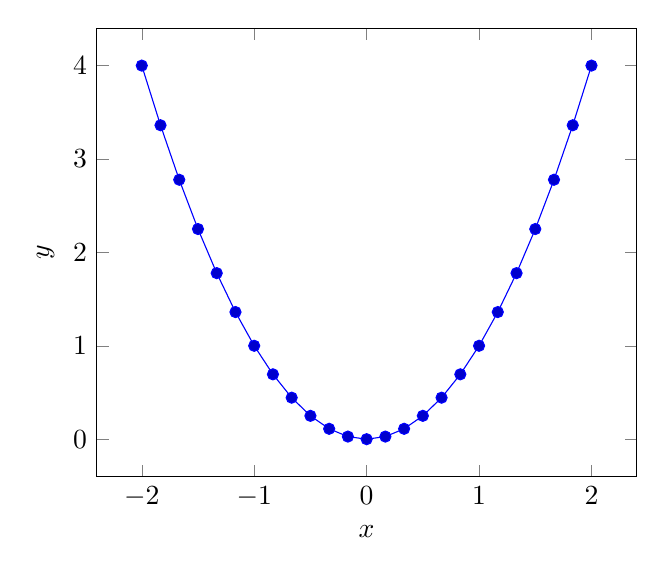
\begin{tikzpicture}
\begin{axis}[
  xlabel={$x$},
  ylabel={$y$},
  domain=-2:2
]
\addplot {x^2};
\end{axis}
\end{tikzpicture}
\end{frame}
\end{lstlisting}

\begin{itemize}
\setlength{\itemsep}{2pt}
\item \texttt{\textbackslash{}begin\{axis\}[...]}：开一个坐标系，方括号里写轴标签和取值范围；
\item \texttt{\textbackslash{}addplot \{x\textasciicircum{}2\};}：画 y = x² 的曲线。对，就是“打字”，跟写公式一个感觉。
\end{itemize}

和插图的取舍一句话说清：\textbf{示意图要经常改就用 TikZ 画，照片、软件导出的数据图还是老老实实插 PDF/PNG}——别用 TikZ 硬画你实验跑出来的折线图，那是给自己找事。

\painhead{Word 做法 vs LaTeX 做法 · 对照小结}

\begin{table}[htbp]
\centering
\small
\begin{tabularx}{\linewidth}{@{}*{3}{>{\raggedright\arraybackslash}X}@{}}
\toprule
\textbf{事项} & \textbf{Word / PowerPoint 做法} & \textbf{LaTeX 做法} \\
\midrule
论文公式搬进幻灯片 & 公式编辑器重打一遍或截图，投影发糊 & 代码原样复制，矢量渲染永不糊 \\
流程图 & SmartArt 套模板，拖线对齐半小时 & TikZ 节点+箭头，改字不动线 \\
换整套风格 & 换母版，元素跑得到处都是 & \texttt{\textbackslash{}usetheme\{\}} 一行换主题 \\
论文和幻灯片的内容同步 & 两套软件两份文件，改一处得改两处 & 同一套代码体系，复制即用 \\
分步出现动画 & 动画面板配半天 & \texttt{\textbackslash{}pause} 一个词（但也别贪多） \\
\bottomrule
\end{tabularx}
\end{table}

\painhead{翻车合集}

\begin{table}[htbp]
\centering
\small
\begin{tabularx}{\linewidth}{@{}*{3}{>{\raggedright\arraybackslash}X}@{}}
\toprule
\textbf{症状} & \textbf{原因} & \textbf{解法} \\
\midrule
中文显示乱码或空白 & 用了 \texttt{beamer} 而不是 \texttt{ctexbeamer}，或引擎没选 XeLaTeX & 文档类换 \texttt{ctexbeamer}，引擎选 XeLaTeX \\
内容超出页面，下面被裁掉 & 一页塞太多，beamer 不会自动缩 & 拆成两页 frame；宁可少放字 \\
演示时内容一页页蹦，收不住 & \texttt{\textbackslash{}pause} 加太多，忘了删 & 全局搜 \texttt{\textbackslash{}pause}，删到一页最多一两个 \\
\texttt{! I can't find file 'tikz.sty'} 之类 & 忘了 \texttt{\textbackslash{}usepackage\{tikz\}} 或写错库名 & 检查导言区，库名按本章原样抄 \\
图表编号显示"??" & 编译了一遍 & 再点一次排版按钮，老规矩（第 5 章讲过） \\
TikZ 节点重叠成一坨 & 忘了 \texttt{positioning} 库，或没用 \texttt{right=of} 语法 & 加 \texttt{\textbackslash{}usetikzlibrary\{positioning\}}，节点用相对定位 \\
\bottomrule
\end{tabularx}
\end{table}

\section*{练习}

\begin{enumerate}
\setlength{\itemsep}{2pt}
\item 用 \texttt{ctexbeamer} + \texttt{Madrid} 主题做一个 3 页的幻灯片：标题页、目录页、一页正文（随便写点你的课程内容），编译通顺；
\item 把你第 6 章练习里写过的一个行间公式原样搬进 frame，对比一下截图糊不糊——体会矢量渲染的爽；
\item 把 14.6 的三节点流程图抄下来编译成功，然后在“模型训练”和“结果分析”之间插一个新节点“模型调参”，体会加框加箭头有多省事；
\item 给 14.7 的例子改成画 \texttt{sin(x)} 曲线（domain 改成 \texttt{-3.14:3.14}），再给 \texttt{\textbackslash{}addplot} 加个选项 \texttt{[red, thick]} 看看效果；
\item \textbf{故意翻车题}：在一个 frame 里连加五个 \texttt{\textbackslash{}pause} 然后编译，数一数这一页在 PDF 里变成了几页——这就是“打印讲义惨案”的案发现场。以后用 \texttt{\textbackslash{}pause} 之前，先想想这张“残骸”。
\end{enumerate}

到这里，论文、模板、幻灯片你都能一个人包圆了。最后一章来一场综合实战：\textbf{从空白文件到一篇能交的小论文}，把全书学的十八般武艺串成一条流水线。

\chapter{综合实战：从空白到一篇能交的小论文}

\begin{notebox}
最后一战。前面 14 章学的所有招式，这一章一口气用完——从空白文件开始，写出《浅谈大学生熬夜现象的分析》这种戏谑但五脏俱全的小论文。
\end{notebox}

\subsection*{15.0 开场白：把弹药一口气打完}

学开车时教练是分开教的：这周练打方向，下周练踩离合，但真上路那天得一口气连起来。前面 14 章也一样——骨架、公式、图表编号、三线表、参考文献各自练过了，这一章把它们串成一条完整流水线。

目标产物是一篇小论文，题目就叫\textbf{《浅谈大学生熬夜现象的分析》}。别笑，这题目是故意的：结构标准、内容好编、图表公式全都用得上。照着做完，你交课程论文、写数模正文、凑实验报告都是同一套动作。全文共 5 步，每步标了用到第几章，卡住了回去翻。

\textbf{开工前的例行公事}：新建一个文件夹，名字全英文，比如 \texttt{D:\textbackslash{}latex\textbackslash{}paper}。主文件、图片、参考文献库，所有文件都放这里面，一个都不能少。

\section*{第 1 步 搭骨架：先让文档站得住（用到了第 2、3 章）}
\addcontentsline{toc}{section}{第 1 步 搭骨架：先让文档站得住（用到了第 2、3 章）}

新建文件，保存为 \texttt{main.tex}，敲入：

\begin{lstlisting}
\documentclass[UTF8, 12pt, a4paper]{ctexart}
\usepackage{geometry}
\geometry{margin=2.5cm}

\title{浅谈大学生熬夜现象的分析}
\author{张三}
\date{2026年10月}

\begin{document}

\maketitle
\tableofcontents

\end{document}
\end{lstlisting}

引擎选 \textbf{XeLaTeX}，点绿色“排版”按钮。出来一个带标题和目录的 PDF——虽然目录现在是空的（一个 \texttt{\textbackslash{}section} 都还没写）。

\textbf{逐行说两句}：

\begin{itemize}
\setlength{\itemsep}{2pt}
\item \texttt{[UTF8, 12pt, a4paper]}：中文、12 磅字、A4 纸，三个选项一次配齐；
\item \texttt{geometry} 是第 10 章的页边距包，一行 \texttt{margin=2.5cm} 四边全定；
\item \texttt{\textbackslash{}maketitle} 生成标题区，\texttt{\textbackslash{}tableofcontents} 生成目录。
\end{itemize}

\begin{notebox}
\textbf{金句：目录想变新，编译得两遍。} 凡是动了 \texttt{\textbackslash{}section}、\texttt{\textbackslash{}label}、\texttt{\textbackslash{}cite} 这类“被引用”的东西，就再点一次排版按钮。控制台出现 \texttt{Rerun to get cross-references right}，意思就是“麻烦您再按一次”。
\end{notebox}

\section*{第 2 步 填文字和公式：正文就是打字（用到了第 2、6 章）}
\addcontentsline{toc}{section}{第 2 步 填文字和公式：正文就是打字（用到了第 2、6 章）}

在 \texttt{\textbackslash{}tableofcontents} 后面接着写两个 section 和一小段正文：

\begin{lstlisting}
\section{引言}

随着手机屏幕越来越亮，大学生入睡时间越来越晚。
熬夜问题已成为高校学生管理中一个绕不开的话题。
本文将从数据出发，对这一现象进行不严肃但认真的分析。

\section{模型构建}

设平均入睡时间为 $t$，社交软件数为 $n$，可以建立如下关系：

\begin{equation}
  T = \frac{24}{1 + k \cdot n}
  \label{eq:sleep}
\end{equation}

其中 $T$ 为平均睡眠时长，$k$ 为拖延系数（由室友实测标定）。由式~\eqref{eq:sleep} 可知，装的软件越多，睡得越少。
\end{lstlisting}

点排版按钮。正文出现了，公式有了编号 (1)，\texttt{式\textasciitilde{}\textbackslash{}eqref\{eq:sleep\}} 自动变成“式 (1)”——第 6 章 amsmath 的老朋友。

\textbf{注意两个细节}：

\begin{itemize}
\setlength{\itemsep}{2pt}
\item 行内公式用 \texttt{\$...\$}，行间带编号用 \texttt{equation} 环境，第 6 章的规矩，别再混了；
\item \texttt{\textasciitilde{}\textbackslash{}eqref\{...\}} 里的 \texttt{\textasciitilde{}} 是个不换行空格，防止“式”字和“(1)”被拆到两行去。小习惯，大体面。
\end{itemize}

\begin{notebox}
\textbf{金句：编号一律 \texttt{\textbackslash{}label}，引用一律 \texttt{\textbackslash{}ref} / \texttt{\textbackslash{}eqref}。} 全文从头到尾不许出现手打的“(1)”——那是 Word 的老毛病，别带过来。
\end{notebox}

\section*{第 3 步 图和表：让论文看起来像篇论文（用到了第 4、5、7 章）}
\addcontentsline{toc}{section}{第 3 步 图和表：让论文看起来像篇论文（用到了第 4、5、7 章）}

\textbf{插一张图}。先随便找一张 PNG（截图、表情包都行），改名为 \texttt{sleep.png} 放进 \texttt{paper} 文件夹，然后在“模型构建”一节里加：

\begin{lstlisting}
\begin{figure}[htbp]
  \centering
  \includegraphics[width=0.8\textwidth]{sleep.png}
  \caption{某宿舍平均入睡时间变化趋势（示意图）}
  \label{fig:trend}
\end{figure}

如图~\ref{fig:trend} 所示，入睡时间呈明显恶化趋势。
\end{lstlisting}

\texttt{width=0.8\textbackslash{}textwidth} 表示图宽占版心的 80\%，不管原图多大都自动缩放到位；\texttt{[htbp]} 让 LaTeX 自己找不碍事的地方放——第 4 章说过，它比你更会放，别跟它抢。

\textbf{再来一张三线表}。接着加一节“数据分析”：

\begin{lstlisting}
\section{数据分析}

对某宿舍开展为期一周的田野调查，结果如表~\ref{tab:hours} 所示。

\begin{table}[htbp]
  \centering
  \caption{不同年级平均入睡时间与睡眠时长}
  \label{tab:hours}
  \begin{tabular}{lcc}
    \toprule
    年级 & 平均入睡时间 & 平均睡眠时长（小时） \\
    \midrule
    大一 & 00:40 & 6.8 \\
    大二 & 01:10 & 6.2 \\
    大三 & 01:25 & 6.0 \\
    \bottomrule
  \end{tabular}
\end{table}

由表~\ref{tab:hours} 可见，年级越高，睡得越晚，这与作业量、游戏时长和"再刷十分钟"的次数正相关。
\end{lstlisting}

三线表就三条命令：\texttt{\textbackslash{}toprule}、\texttt{\textbackslash{}midrule}、\texttt{\textbackslash{}bottomrule}（第 7 章 booktabs 的三条横线）。竖线？不存在的——学术表格没有竖线，Word 时代画满网格线的日子让它过去吧。

别忘了导言区加两行：

\begin{lstlisting}
\usepackage{graphicx}
\usepackage{booktabs}
\end{lstlisting}

编译两遍（对，又是两遍），图表编号和“图 1”“表 1”的引用全部到位。

\section*{第 4 步 参考文献：机器替你排国标（用到了第 8 章）}
\addcontentsline{toc}{section}{第 4 步 参考文献：机器替你排国标（用到了第 8 章）}

\textbf{第一步：建一个 \texttt{refs.bib} 文件}（注意后缀是 \texttt{.bib} 不是 \texttt{.tex}），内容如下：

\begin{lstlisting}
@article{zhang2023,
  author  = {张明 and 李华},
  title   = {大学生睡眠质量与学业压力的关系研究},
  journal = {中国青年研究},
  year    = {2023},
  number  = {4},
  pages   = {56--61},
}

@book{wang2021,
  author    = {王晓红},
  title     = {大学生健康行为学},
  publisher = {高等教育出版社},
  address   = {北京},
  year      = {2021},
}
\end{lstlisting}

每条文献开头的 \texttt{zhang2023} 是你自己起的\textbf{引用钥匙}，后面全靠它点名。

\textbf{第二步：导言区配置 biblatex}，一键国标格式：

\begin{lstlisting}
\usepackage[backend=biber, style=gb7714-2015]{biblatex}
\addbibresource{refs.bib}
\end{lstlisting}

\texttt{style=gb7714-2015} 就是 GB/T 7714—2015 国家标准，导师要的国标格式，四个词搞定——第 8 章手打一下午的痛，到此为止。

\textbf{第三步：在正文里引用}，比如在“数据分析”末尾加一句：

\begin{lstlisting}
已有研究表明，睡眠不足与学业表现呈负相关~\cite{zhang2023}。
\end{lstlisting}

\textbf{第四步：在正文最后、\texttt{\textbackslash{}end\{document\}} 之前，打印文献列表}：

\begin{lstlisting}
\printbibliography
\end{lstlisting}

\textbf{第五步：完整编译顺序}。用了 biber 就不能只按一个按钮了，按这个顺序来：

\begin{lstlisting}
XeLaTeX  →  biber  →  XeLaTeX  →  XeLaTeX
\end{lstlisting}

具体操作：第一遍正常点排版按钮（引擎 XeLaTeX）；然后引擎下拉菜单切换成 \textbf{Biber}，再点一次；最后换回 XeLaTeX 连点两遍。四遍过后，文中的 \texttt{[1]} 和文末的“参考文献”列表整整齐齐，全是国标格式。

\begin{notebox}
\textbf{金句：.bib 存一次，格式是机器的事。} 以后要换格式？改 \texttt{style=} 一个词，完事。
\end{notebox}

\section*{第 5 步 定稿检查清单：交稿前过一遍}
\addcontentsline{toc}{section}{第 5 步 定稿检查清单：交稿前过一遍}

交 PDF 前逐条打勾，这份清单能救你于导师的红笔之下：

\begin{enumerate}
\setlength{\itemsep}{2pt}
\item \textbf{全文搜“？?”}——出现“？?”说明有引用没编出来，再编译一遍，或检查 \texttt{\textbackslash{}label} 是否写在了 \texttt{\textbackslash{}caption} 后面（第 5 章的坑）；
\item \textbf{目录是不是最新的}——删过章节、改过标题的，必须再编译两遍；
\item \textbf{图片是不是都出来了}——逐页看一眼；“图跑到文档最后去了”是浮动体的正常行为，用 \texttt{[htbp]}，并检查图片文件名（大小写也要对）；
\item \textbf{字号字体}——\texttt{12pt} 是否真写进了文档类选项，别靠肉眼看；
\item \textbf{导出 PDF 检查页边距}——用 PDF 阅读器打开 \texttt{main.pdf}（别用 TeXworks 内置预览）通读一遍，页边距、页码、断行全见真章。
\end{enumerate}

全过，就可以交了。恭喜，你刚用 LaTeX 写完了一篇完整论文——全程没有一步是“手动改编号”。

\subsection*{15.6 完整成品：main.tex 全文}

上面是分段讲的，这里是拼好的整份。\texttt{paper} 文件夹里放 \texttt{main.tex}、\texttt{refs.bib}、\texttt{sleep.png} 三个文件，即可编译。

\begin{lstlisting}
\documentclass[UTF8, 12pt, a4paper]{ctexart}
\usepackage{geometry}
\geometry{margin=2.5cm}
\usepackage{graphicx}
\usepackage{booktabs}
\usepackage{amsmath}
\usepackage[backend=biber, style=gb7714-2015]{biblatex}
\addbibresource{refs.bib}

\title{浅谈大学生熬夜现象的分析}
\author{张三}
\date{2026年10月}

\begin{document}

\maketitle
\tableofcontents

\section{引言}

随着手机屏幕越来越亮，大学生入睡时间越来越晚。熬夜问题已成为高校学生管理中一个绕不开的话题。本文将从数据出发，对这一现象进行不严肃但认真的分析。

\section{模型构建}

设平均入睡时间为 $t$，社交软件数为 $n$，可以建立如下关系：

\begin{equation}
  T = \frac{24}{1 + k \cdot n}
  \label{eq:sleep}
\end{equation}

其中 $T$ 为平均睡眠时长，$k$ 为拖延系数（由室友实测标定）。由式~\eqref{eq:sleep} 可知，装的软件越多，睡得越少。

\begin{figure}[htbp]
  \centering
  \includegraphics[width=0.8\textwidth]{sleep.png}
  \caption{某宿舍平均入睡时间变化趋势（示意图）}
  \label{fig:trend}
\end{figure}

如图~\ref{fig:trend} 所示，入睡时间呈明显恶化趋势。

\section{数据分析}

对某宿舍开展为期一周的田野调查，结果如表~\ref{tab:hours} 所示。

\begin{table}[htbp]
  \centering
  \caption{不同年级平均入睡时间与睡眠时长}
  \label{tab:hours}
  \begin{tabular}{lcc}
    \toprule
    年级 & 平均入睡时间 & 平均睡眠时长（小时） \\
    \midrule
    大一 & 00:40 & 6.8 \\
    大二 & 01:10 & 6.2 \\
    大三 & 01:25 & 6.0 \\
    \bottomrule
  \end{tabular}
\end{table}

由表~\ref{tab:hours} 可见，年级越高，睡得越晚，这与作业量、游戏时长和"再刷十分钟"的次数正相关。

已有研究表明，睡眠不足与学业表现呈负相关~\cite{zhang2023}。

\printbibliography

\end{document}
\end{lstlisting}

编译口诀再念一遍：\textbf{XeLaTeX \ensuremath{\rightarrow} biber \ensuremath{\rightarrow} XeLaTeX \ensuremath{\rightarrow} XeLaTeX}。四遍之后，一篇有标题、有目录、有公式、有图表、有国标参考文献的小论文就躺在你文件夹里了。

到这里，这本书教的招式你已经全部实战过了。但我们都懂一个真理：\textbf{学会了不等于不出错}。一编译，控制台还是可能蹦出一句看不懂的天书。

别慌。下一章是全书最后的\textbf{急救手册}——20 个最常见报错逐条给修法，外加一整套速查表。以后卡住了就翻它，不用从头翻书。

\chapter{急救手册：报错、速查与保命技巧}

\begin{notebox}
本章不需要从头读到尾。它是工具箱：报错了翻第一节，想要效果翻第二节，忘了命令翻第三节。建议收藏，长期有效。
\end{notebox}

\section*{一、20 个最常见报错逐条修}

读报错的通用姿势：\textbf{先找第一个 \texttt{!} 开头的行，再看它下面 \texttt{l.数字} 定位到源码第几行}。后面的错误多半是连坐，改完第一条再说。另有两条万能招：大括号是否成对、\texttt{\$} 是否成对。

\textbf{1.}

\begin{lstlisting}
! Undefined control sequence.
l.15 \includegrophics
\end{lstlisting}

原因：命令拼错了，LaTeX 不认识 \texttt{\textbackslash{}includegrophics}。修复：对照正确拼写改 \texttt{l.15} 那行，大小写也要对（正确是 \texttt{\textbackslash{}includegraphics}）。

\textbf{2.}

\begin{lstlisting}
! Missing $ inserted.
\end{lstlisting}

原因：正文里用了数学符号（\texttt{\_}、\texttt{\textasciicircum{}}、希腊字母等），却没包进 \texttt{\$...\$}。修复：用 \texttt{\$...\$} 包起来；真想打下划线字符，写 \texttt{\textbackslash{}\_}。

\textbf{3.}

\begin{lstlisting}
! LaTeX Error: File `booktabs.sty' not found.
! LaTeX Error: File `sleep.png' not found.
\end{lstlisting}

原因：找不到文件——\texttt{.sty} 是宏包没装，\texttt{.png} 是图片不在文件夹里或文件名大小写不对。修复：缺包在命令行运行 \texttt{tlmgr install booktabs}（包名去掉 .sty）；图片检查是否和 main.tex 同文件夹、文件名一字不差。

\textbf{4.}

\begin{lstlisting}
! Extra alignment tab has been changed to \cr.
\end{lstlisting}

原因：表格某行的 \texttt{\&} 比列数多了一个。修复：\texttt{\textbackslash{}begin\{tabular\}\{lcc\}} 是 3 列，每行最多 2 个 \texttt{\&}，删掉多的。

\textbf{5.}

\begin{lstlisting}
! Misplaced alignment tab character &.
\end{lstlisting}

原因：\texttt{\&} 跑到表格环境外面来了。修复：正文里想打 \& 符号写 \texttt{\textbackslash{}\&}；多余的 \texttt{\&} 删掉。

\textbf{6.}

\begin{lstlisting}
! LaTeX Error: Missing \begin{document}.
\end{lstlisting}

原因：\texttt{\textbackslash{}begin\{document\}} 之前出现了正文内容——手滑在导言区打了字，或混进了看不见的中文全角空格。修复：检查 \texttt{\textbackslash{}begin\{document\}} 前是不是只有命令和注释；可疑行删了重打。

\textbf{7.}

\begin{lstlisting}
! LaTeX Error: \begin{figure} on input line 12 ended by \end{table}.
\end{lstlisting}

原因：环境名前后不匹配——\texttt{\textbackslash{}begin\{figure\}} 开头，却用 \texttt{\textbackslash{}end\{table\}} 收尾。修复：\texttt{\textbackslash{}begin\{什么\}} 就得 \texttt{\textbackslash{}end\{什么\}}，复制粘贴环境时最容易犯。

\textbf{8.}

\begin{lstlisting}
! Missing } inserted.
\end{lstlisting}

原因：大括号没闭合，话说了一半。修复：顺着 \texttt{l.行号} 往前找，补上 \texttt{\}}。好习惯：打 \texttt{\{} 时立刻打 \texttt{\}}，再往中间填内容。

\textbf{9.}

\begin{lstlisting}
LaTeX Warning: Float too large for page by 15.3pt.
\end{lstlisting}

原因：图太大，超出页面高度（是警告，但结果往往是图被截断）。修复：\texttt{width=0.8\textbackslash{}textwidth} 改小，或超高图改用 \texttt{height=0.7\textbackslash{}textheight} 控制。

\textbf{10.}

\begin{lstlisting}
! LaTeX Error: Environment align undefined.
\end{lstlisting}

原因：用了 \texttt{align} 等数学环境，但没加载 amsmath。修复：导言区加 \texttt{\textbackslash{}usepackage\{amsmath\}}。

\textbf{11.}

\begin{lstlisting}
LaTeX Warning: Reference `fig:trend' on page 2 undefined on input line 20.
\end{lstlisting}

原因：\texttt{\textbackslash{}ref\{fig:trend\}} 找不到对应的 \texttt{\textbackslash{}label\{fig:trend\}}——名字拼错，或还没编译两遍。修复：核对名字一字不差，再编译一遍；PDF 里的“？?”多半就是它。

\textbf{12.}

\begin{lstlisting}
LaTeX Warning: Citation `zhang2023' undefined on input line 30.
\end{lstlisting}

原因：\texttt{\textbackslash{}cite} 的钥匙在 refs.bib 里找不到，或还没跑 biber。修复：核对钥匙名，按完整顺序 \textbf{XeLaTeX \ensuremath{\rightarrow} biber \ensuremath{\rightarrow} XeLaTeX \ensuremath{\rightarrow} XeLaTeX} 重编。

\textbf{13.}

\begin{lstlisting}
! Emergency stop.
\end{lstlisting}

原因：紧急刹车，本身不是病因，是 LaTeX 中途罢工的告别语。修复：往上翻，找第一条 \texttt{!} 行，按那一条修。

\textbf{14.}

\begin{lstlisting}
Runaway argument?
{ ...
! File ended while scanning use of \frac.
\end{lstlisting}

原因：某命令的参数没闭合就到了文件结尾。修复：检查报错点名的命令（这里是 \texttt{\textbackslash{}frac}），补上配对的 \texttt{\}}。

\textbf{15.}

\begin{lstlisting}
! Missing number, treated as zero.
\end{lstlisting}

原因：某命令需要数字（长度、尺寸），你却没给。修复：按 \texttt{l.行号} 找到该命令，补全数字和单位。

\textbf{16.}

\begin{lstlisting}
! Illegal unit of measure (pt inserted).
\end{lstlisting}

原因：长度后面没写单位，LaTeX 只好默认 pt——\texttt{\textbackslash{}vspace\{2\}} 少了 \texttt{cm} 就是这种。修复：给所有长度补上单位（cm/mm/pt）或补上 \texttt{\textbackslash{}textwidth} 这类参照。

\textbf{17.}

\begin{lstlisting}
! LaTeX Error: Option clash for package xcolor.
\end{lstlisting}

原因：同一个宏包被 \texttt{\textbackslash{}usepackage} 了两次且选项不一致。修复：全文搜宏包名，把两次加载合并成一次。用别人模板时常犯。

\textbf{18.}

\begin{lstlisting}
! I'm skipping whatever remains of this command.
\end{lstlisting}

原因：命令的参数没写完就断了——多半是参数里出现了空行，或 \texttt{\textbackslash{}verb} 命令跨了行。修复：删掉参数里的空行；\texttt{\textbackslash{}verb} 只写在一行内。

\textbf{19.}

\begin{lstlisting}
! Package inputenc Error: Unicode character 张 (U+5F20) not set up for use with LaTeX.
\end{lstlisting}

原因：引擎选错了，pdfLaTeX 编不了中文——新手第一大坑。修复：TeXworks 引擎下拉菜单换成 \textbf{XeLaTeX} 重新编译。一句话：\textbf{写中文，XeLaTeX，别问。}

\textbf{20.}

\begin{lstlisting}
*
(Please type a command or say \end)
\end{lstlisting}

原因：控制台停住等你输入——之前的错误把 LaTeX 带进了交互模式。修复：控制台里按\textbf{回车}跳过，或点红色 \ensuremath{\times} 终止，改完代码重来。回车只是让流程走完，不解决问题本身。

\section*{二、“我想要 X 效果”速查索引}

照抄即可，宏包都加在导言区（\texttt{\textbackslash{}begin\{document\}} 之前）。

\begin{table}[htbp]
\centering
\small
\begin{tabularx}{\linewidth}{@{}*{2}{>{\raggedright\arraybackslash}X}@{}}
\toprule
\textbf{我想要} & \textbf{怎么做} \\
\midrule
正文两端对齐 & \texttt{ctexart} 默认就是，什么都不用做 \\
文字加删除线 & 导言区 \texttt{\textbackslash{}usepackage[normalem]\{ulem\}}，正文 \texttt{\textbackslash{}sout\{不要的话划掉\}} \\
彩色文字 & 导言区 \texttt{\textbackslash{}usepackage\{xcolor\}}，正文 \texttt{\textbackslash{}textcolor\{red\}\{重点\}} \\
代码高亮 & 导言区 \texttt{\textbackslash{}usepackage\{listings\}}，正文用 \texttt{lstlisting} 环境包代码（见下方例子） \\
标题不编号但进目录 & \texttt{\textbackslash{}section*\{致谢\}} 后紧跟 \texttt{\textbackslash{}addcontentsline\{toc\}\{section\}\{致谢\}} \\
页码罗马数字转阿拉伯 & 正文开始处 \texttt{\textbackslash{}pagenumbering\{roman\}}，之后换 \texttt{\textbackslash{}pagenumbering\{arabic\}} \\
图别乱跑，就在原地 & 导言区 \texttt{\textbackslash{}usepackage\{float\}}，figure 环境的位置改成 \texttt{[H]} \\
加一段垂直空白 & 正文里 \texttt{\textbackslash{}vspace\{1cm\}}（记得带单位） \\
某段不缩进 & 该段开头 \texttt{\textbackslash{}noindent} \\
给一句话加边框 & 正文 \texttt{\textbackslash{}fbox\{这里被框起来了\}} \\
重点提示框（带底色） & 导言区 \texttt{\textbackslash{}usepackage\{tcolorbox\}}，正文用 \texttt{\textbackslash{}begin\{tcolorbox\}内容\textbackslash{}end\{tcolorbox\}} \\
1.5 倍行距 & 导言区 \texttt{\textbackslash{}usepackage\{setspace\}}，正文区开头 \texttt{\textbackslash{}onehalfspacing} \\
页眉页脚自定义 & 导言区 \texttt{\textbackslash{}usepackage\{fancyhdr\}}（第 10 章有完整例子） \\
引用能点击跳转、不带红框 & 导言区最后一条 \texttt{\textbackslash{}usepackage[hidelinks]\{hyperref\}} \\
\bottomrule
\end{tabularx}
\end{table}

代码高亮最小完整例子：

\begin{lstlisting}
\documentclass[UTF8]{ctexart}
\usepackage{listings}
\begin{document}

\begin{lstlisting}
def main():
    print("hello")
\end{lstlisting}

\end{document}
\end{lstlisting}

\section*{三、包速查表 + 符号速查}

\subsubsection*{常用宏包}

\begin{table}[htbp]
\centering
\small
\begin{tabularx}{\linewidth}{@{}*{3}{>{\raggedright\arraybackslash}X}@{}}
\toprule
\textbf{宏包} & \textbf{一句话说明} & \textbf{典型用法} \\
\midrule
\texttt{ctex} & 中文支持（ctexart 文档类自动带） & \texttt{\textbackslash{}documentclass[UTF8]\{ctexart\}} \\
\texttt{graphicx} & 插图 & \texttt{\textbackslash{}includegraphics[width=0.8\textbackslash{}textwidth]\{a.png\}} \\
\texttt{amsmath} & 公式增强（align、\textbackslash{}eqref 靠它） & \texttt{\textbackslash{}usepackage\{amsmath\}} \\
\texttt{booktabs} & 三线表三条线 & \texttt{\textbackslash{}toprule \textbackslash{}midrule \textbackslash{}bottomrule} \\
\texttt{biblatex} & 参考文献（配 biber） & \texttt{\textbackslash{}usepackage[backend=biber, style=gb7714-2015]\{biblatex\}} \\
\texttt{geometry} & 页边距 & \texttt{\textbackslash{}geometry\{margin=2.5cm\}} \\
\texttt{xcolor} & 颜色 & \texttt{\textbackslash{}textcolor\{blue\}\{字\}} \\
\texttt{float} & 强制图片位置 & figure 环境用 \texttt{[H]} \\
\texttt{hyperref} & 引用变超链接（永远最后加载） & \texttt{\textbackslash{}usepackage[hidelinks]\{hyperref\}} \\
\texttt{subcaption} & 并排子图 & \texttt{\textbackslash{}begin\{subfigure\}\{0.48\textbackslash{}textwidth\}} \\
\texttt{ulem} & 删除线 & \texttt{\textbackslash{}sout\{划掉\}} \\
\texttt{setspace} & 行距 & \texttt{\textbackslash{}onehalfspacing} \\
\texttt{fancyhdr} & 页眉页脚 & 第 10 章 \\
\texttt{listings} & 代码排版 & 第二节有最小例 \\
\texttt{tcolorbox} & 彩色提示框 & 第二节有用法 \\
\bottomrule
\end{tabularx}
\end{table}

\subsubsection*{常用数学符号}

用法统一是 \texttt{\$ 符号 \$}，比如 \texttt{\$\textbackslash{}alpha\$} 出 \ensuremath{\alpha}。

\begin{table}[htbp]
\centering
\small
\begin{tabularx}{\linewidth}{@{}*{4}{>{\raggedright\arraybackslash}X}@{}}
\toprule
\textbf{符号} & \textbf{命令} & \textbf{符号} & \textbf{命令} \\
\midrule
\ensuremath{\alpha} & \texttt{\textbackslash{}alpha} & \ensuremath{\beta} & \texttt{\textbackslash{}beta} \\
\ensuremath{\gamma} & \texttt{\textbackslash{}gamma} & \ensuremath{\delta} & \texttt{\textbackslash{}delta} \\
\ensuremath{\theta} & \texttt{\textbackslash{}theta} & \ensuremath{\lambda} & \texttt{\textbackslash{}lambda} \\
\ensuremath{\mu} & \texttt{\textbackslash{}mu} & \ensuremath{\sigma} & \texttt{\textbackslash{}sigma} \\
\ensuremath{\pi} & \texttt{\textbackslash{}pi} & \ensuremath{\omega} & \texttt{\textbackslash{}omega} \\
\ensuremath{\Delta} & \texttt{\textbackslash{}Delta} & \ensuremath{\Omega} & \texttt{\textbackslash{}Omega} \\
\ensuremath{\Sigma}（求和） & \texttt{\textbackslash{}sum} & \ensuremath{\int}（积分） & \texttt{\textbackslash{}int} \\
\ensuremath{\partial} & \texttt{\textbackslash{}partial} & \ensuremath{\infty} & \texttt{\textbackslash{}infty} \\
\ensuremath{\leq} & \texttt{\textbackslash{}leq} & \ensuremath{\geq} & \texttt{\textbackslash{}geq} \\
\ensuremath{\neq} & \texttt{\textbackslash{}neq} & \ensuremath{\approx} & \texttt{\textbackslash{}approx} \\
\ensuremath{\pm} & \texttt{\textbackslash{}pm} & \ensuremath{\times} & \texttt{\textbackslash{}times} \\
\ensuremath{\rightarrow} & \texttt{\textbackslash{}rightarrow} & \ensuremath{\Rightarrow} & \texttt{\textbackslash{}Rightarrow} \\
\ensuremath{\leftrightarrow} & \texttt{\textbackslash{}leftrightarrow} & \ensuremath{\Leftrightarrow} & \texttt{\textbackslash{}Leftrightarrow} \\
\ensuremath{\in} & \texttt{\textbackslash{}in} & \ensuremath{\notin} & \texttt{\textbackslash{}notin} \\
\ensuremath{\subset} & \texttt{\textbackslash{}subset} & \ensuremath{\cup} / \ensuremath{\cap} & \texttt{\textbackslash{}cup} / \texttt{\textbackslash{}cap} \\
\ensuremath{\forall} & \texttt{\textbackslash{}forall} & \ensuremath{\exists} & \texttt{\textbackslash{}exists} \\
\bottomrule
\end{tabularx}
\end{table}

\begin{notebox}
想不到符号命令？画出来认——第 6 章提过：拿鼠标在 detexify 网站上画一笔，它猜给你命令。这张表覆盖日常 90\%，剩下的交给它。
\end{notebox}

\subsubsection*{TeXworks 保命技巧}

\begin{itemize}
\setlength{\itemsep}{2pt}
\item \textbf{Tab 补全}：敲 \texttt{\textbackslash{}begin} 后按 Tab 能补全命令。不用背全拼，敲前几个字母按 Tab 试探，效率翻倍；
\item \textbf{源码与 PDF 互跳}：按住 \textbf{Ctrl} 点击源码，PDF 跳到对应位置；反过来 Ctrl+点击 PDF 也能跳回源码（SyncTeX）。百页文档找错全靠它；
\item \textbf{常用快捷键}：\texttt{Ctrl + S} 保存（编译前必须存，TeXworks 编的是硬盘上的文件，不保存等于白改）、\texttt{Ctrl + F} 查找、\texttt{Ctrl + T} 注释选中行 / \texttt{Ctrl + U} 取消注释（排查错误时把可疑行注释掉再看，神器）；
\item \textbf{控制台“按回车继续”}：看到 \texttt{(Please type a command or say \textbackslash{}end)} 就按回车跳过，或红 \ensuremath{\times} 终止重来。报错没修好之前，按一百次回车也编不出正确结果。
\end{itemize}

\section*{结语}

全书到此结束。

回头看看：14 章前你还在为改一个标题格式、刷一遍目录、手打一版参考文献发愁；现在你能从空白文件出发，一路敲出一篇带公式、图表和国标文献的完整论文——而且从今往后，改内容不用再碰格式，编号永远自己排队，参考文献永远是国标。

这就是 LaTeX 和 Word 最本质的区别：\textbf{Word 里，格式是你的事；LaTeX 里，格式是它的事。}

从今天起，格式的事，让它自己干。你只管把内容写好。

本手册独立可查、长期有效——以后卡住了，先翻第一节对报错，再翻第二节找效果，包和符号忘了就在第三节捞。祝你以后的每一篇文档，都一次编译通过。

（好吧，两次。记得编译两遍。）


\end{document}
